%äöüß

\documentclass[                 % Koma: scrartcl, srcreprt, srcbook, scrlttr2
12pt                           % 10pt, 11pt, 12pt
% ,draft                         % draft/final
%TODO
,twoside                        % one/two: different layout for left/right pages
%
,onecolumn                      % one/two
%,fleqn                          % equations aligned left
,english                        %
,titlepage                      % titlepage / notitlepage = title on a page of its own
%,noonelinecaption              % table + figure captions of only one line are not treated different
% to multiline-ones
,openany                        % openright : new chapters only on right pages, openany: do not care
% only for scrreprt and scrbook, not scrartcl
,headsepline=true
,headings=big % big normal small
,toc=listof % LOF + LOT
%,toc=listofnumbered
,toc=bibliography
%,toc=bibliographynumbered
%,toc=index  % Fügt das Stichwortverzeichnis ins Inhaltsverzeichnis ein.
,parskip=half- % false, full, half, with -+* behind as modifier
]{scrbook}

\usepackage[utf8]{inputenc}     % Umlaute (Linux)
%\usepackage[latin1]{inputenc}  % Umlaute (Windows)
\usepackage[T1]{fontenc}        % Worttrennung von Worten mit Umlauten möglich

\newcommand{\Verfasser}{Torben Menke}
\newcommand{\Titel}{Molecular Doping of Organic Semiconductors - A Conductivity and Seebeck Study}
%äöüß

% compress PDF, already default, so not needed any more
\pdfminorversion=5
\pdfobjcompresslevel=3 
\pdfcompresslevel=9

% Deutsche Sprache:
%\usepackage{ngerman} % ngerman, german
% Englische Sprache mit Deutschen Abschnitten: %
\usepackage[ngerman,american]{babel} % american , british
% Englische Sprache: %
% \usepackage[american]{babel} % american , british

% nun via \usepackage{tud-font-tm}
% Schriften von Hand wählen: Bsp= Palatino
% \renewcommand{\rmdefault}{ppl}
% \renewcommand{\sfdefault}{phv}
% \renewcommand{\ttdefault}{pcr}
% Sans Serif statt roman als default:
% \renewcommand*\familydefault{\sfdefault}

% Definitions
% =================
% Seperate paragraphs by an empty line instead of intending the line
% old:
%\setlength{\parskip}{2ex plus0.5ex minus0.3ex}
%\setlength{\parindent}{0pt}
% nun via KoMa Option parskip in DocClass

% put subsubsections in toc
\setcounter{secnumdepth}{3}
\setcounter{tocdepth}{3}

% layout of Captions in Tables and Figures (Bildunterschriften)
% \setkomafont{caption}{\small\sffamily}    % Font of the Caption \itshape
\setkomafont{caption}{\small\itshape}    % Font of the Caption \itshape
\setkomafont{captionlabel}{\bfseries}     % Font of the Label 'Figure' etc
\setcapindent{0em}                        % decrease intention of following lines
% \setcapwidth[c]{0.9\textwidth}            % NOTE: makes problems with package sidecap
% hence done manually in each figure using the following width:

\renewcommand{\topfraction}{.80} % up to 80% of page (from top) are allowed to be covered by a float until a float[t] page [p] is generated.

\renewcommand{\bottomfraction}{.80}% up to 40% of page (from bottom) are allowed to be covered by a float[b] until a float page [p] is generated.

% \renewcommand{\textfraction}{.2} %-> soviel muss text sein

\usepackage{amsmath}     % reqno: equation numbers right hand side of the eq
%\usepackage{amssymb} % \mathfrak does not word here :-( (font eufm10 missing)
%\usepackage{mathrsfs} % for \mathscr{ASDF}

\usepackage{geometry}           % Pagesettings
% Print: left=4cm
% online: left=3cm
% TODO: Print: Verlag Dr. Hut: left=2.7cm
% \geometry{left=2.7cm,textwidth=15cm,top=3cm,textheight=23.5cm}
\geometry{left=3.0cm,textwidth=15cm,top=3cm,textheight=23.5cm}

\newdimen\tmCapWidth
\advance\tmCapWidth by 1.0\textwidth

\usepackage[automark]{scrpage2}
%Clear
\ofoot[]{}
\cfoot[]{}
\ifoot[]{}
\ohead[]{}
\chead[]{}
\ihead[]{}

\setkomafont{pageheadfoot}{\small\sffamily}%\itshape

% \setkomafont{pageheadfoot}{\itshape} % klappt nicht, daher siehe unten
\setkomafont{pagenumber}{\small\sffamily}% aktivieren, falls die Seitenzahl kursiv soll

% \pagemark \headmark
\ihead[]{\headmark} % \itshape
\ohead[\pagemark]{\pagemark}

% \chead%
% [\footnotesize Stand: \the\day.\the\month.\the\year]
% {\footnotesize Stand: \the\day.\the\month.\the\year}
% \today -> EN format :-(

\pagestyle{scrheadings}

% Set Footnote symbols to symbols instead of numbers
\usepackage[perpage,symbol*]{footmisc} % perpage = reset counter on each page
% Latex Default = \DefineFNsymbols*{lamport}{*\dagger\ddagger\S\P|{**}{\dagger\dagger}{\ddagger\ddagger}}
\DefineFNsymbols*{TorbensFN}[math]{\ddagger\Sorg\P\dagger\ast{\dagger\dagger}{\ddagger\ddagger}{\ast\ast}{\Sorg\Sorg}{\P\P}}
% \|
% * wird nicht angezeigt und \S habe ich überschrieben, daher \Sorg
\setfnsymbol{TorbensFN}
% \setfnsymbol{wiley}

% http://web.slzm.de/blog/latex/schone-kapiteltitelseiten-in-latex/
\usepackage[table,dvipsnames,svgnames]{xcolor}
% \usepackage{blindtext}
% \usepackage{fix-cm}
\usepackage{titlesec}
% Style 1
%\renewcommand{\thechapter}{\Roman{chapter}}
\titleformat{\chapter}[display]
{\sffamily\bfseries}%\Large
{ %\Huge\textsc{\chaptertitlename}
\selectfont\color{gray}\hfill %lightgray
\begin{rotate}{90}
%\hspace{0.4cm}
\Large\selectfont \chaptertitlename
\end{rotate}
% \chaptertitlename \hspace*{0.0ex}
\fontsize{90}{70}\sffamily\textbf{\thechapter}}
{-2ex}%{-2ex}
{
\filleft\fontsize{30}{30}\selectfont\sffamily%\scshape
% \phantom{l}\phantom{g}invisible chars for fixing jumping of chapter name
}
[\vspace{0ex}\phantom{l}]

\usepackage[section]{placeins}
% defines the command \FloatBarrier: the name is program
% [section] : floats are not allowed to travel into another section

\usepackage[pdftex]{graphicx}
\usepackage{wrapfig}
% \begin{wrapfigure}{r}{21mm}%
% {\includegraphics{}\caption{}\label{}}%
% \end{wrapfigure}%
\usepackage[outercaption] {sidecap} % Caption besides the figure

\usepackage{pdfpages}
% \includepdf[pages=1-4,pagecommand={\thispagestyle{headings}}]{Meindoku.pdf}

% ===FONTS=== (vor siunitx laden!)

% %=== Variante 1: TUD CD ====
% % nicht VERGESSEN: set \sffamily after \begin{Document}
% \pdfmapfile{=univers.map} % von Hand laden, wenn map nicht registriert, muss in diesem Ordner liegen
% \usepackage[
% tudcd % TUD CD Universe
% %cm % Computer Modern
% %cmbright % CM-Bright fonts
% %helvet % Helvetiva
% %tx % Postscript txfonts
% %px % Postscript pxfonts
% %%lm % Latin Modern DOES NOT WORK WITHOUT FURTHER PACKAGES
% %,slantedGreek % -> slanted \ohm :-(
% %,T1experimental % = ???
% ]{tud-font-tm}
% % 2. Font DinBold manuell für Sections etc via \dinBold im Titel
% \pdfmapfile{=dinbold.map}
% \newcommand*{\dinBold}{\fontencoding{T1}\fontfamily{din}\fontseries{b}\upshape\selectfont}
% !!!TODO!!! for TU Font Universe
% \sisetup{obeyfamily=false,mathrm=mathsf,textrm=sffamily}
%\sisetup{detect-family = true} % for new versions of siunitx

%==== Variante 2: Charter + BeraSans====
% \usepackage{berasans} % = \renewcommand{\sfdefault}{fvs}
\usepackage{charter} % Bitstream Charter, mdbch
\usepackage[charter]{mathdesign} % replaces mathrsfs
\usepackage{beramono}
% Classico a.k.a. Optima as non-serif font
\pdfmapfile{=uop.map}
\renewcommand{\sfdefault}{uop} % Classico a.k.a. Optima

%==== Variante 3: Garamond & Classico Optima====
% \renewcommand{\rmdefault}{ugm} % Garamond
% \pdfmapfile{=uop.map}
% \renewcommand{\sfdefault}{uop} % Classico a.k.a. Optima
% \usepackage[garamond]{mathdesign}
% installed via
% http://my.opera.com/freedo/blog/2008/09/04/wie-kommt-die-garamond-ins-latex
% 1. getnonfreefonts -l
% 2. getnonfreefonts -d classico garamond
% 3. updmap

% === select font for headings
% \addtokomafont{title}        {\fontfamily{uop}}
% \addtokomafont{subtitle}     {\fontfamily{uop}}
% \addtokomafont{chapter}      {\fontfamily{uop}}
% \addtokomafont{section}      {\fontfamily{uop}}
% \addtokomafont{subsection}   {\fontfamily{uop}}
% \addtokomafont{subsubsection}{\fontfamily{uop}}
% könnte Probleme machen, weil umdefinierungen...
% besser nur sowas wie \normalfont \sffamily \mdseries

% Fonts VOR siunitx laden!
%\usepackage{textcomp} % Symbols like (C) etc, allows wring of °C and µ in text

% % http://www.mrunix.de/forums/archive/index.php/t-47484.html
% % mag diesen Satz + luximono statt courier
% \usepackage{berasans} % = \renewcommand{\sfdefault}{fvs}
% \usepackage{charter} % Bitstream Charter, mdbch
% \usepackage[charter]{mathdesign} % replaces mathrsfs
% \usepackage[scaled=1.1]{beramono}

% \usepackage{courier} % typewriter font
% % \usepackage{beraserif}
% % \usepackage{luximono} % typewriter font

%\usepackage{eulervm}

% % Palatino
% \usepackage{mathpazo}
% \usepackage[scaled=.95]{helvet}
% \usepackage{courier}

% % Times
% \usepackage{mathptmx}
% \usepackage[scaled=.92]{helvet}
% \usepackage{courier}

% \usepackage{bookman}

% \usepackage{newcent}

% http://my.opera.com/freedo/blog/2008/09/04/wie-kommt-die-garamond-ins-latex
% 1. getnonfreefonts -l
% 2. getnonfreefonts -d classico garamond
% 3. updmap

% \renewcommand{\rmdefault}{ugm} % Garamond
% \pdfmapfile{=uop.map}
% \renewcommand{\sfdefault}{uop} % Classico a.k.a. Optima
% \usepackage[garamond]{mathdesign}
% %\renewcommand{\ttdefault}{pcr}

%\usepackage{garamond}

% %\usepackage{dinbold}
% % \dinbold
% %\renewcommand*{\seriesdefault}{b}
% \pdfmapfile{=dinbold.map}
% \renewcommand{\sfdefault}{din}
% % \renewcommand{\bfdefault}{b}
% %\renewcommand{\rmdefault}{din}
% % \renewcommand{\ttdefault}{pcr}
% %\renewcommand{\mddefault}{l}

\usepackage{xfrac} % load before siunitx to allow for sfrac

\usepackage[
abbreviations = false
,noload={abbr} % \mm
,load={prefix,named,physical,accepted,addn} % no linebreaks or spacing here!
%prefix   \kilometer \milli
%named    \celsius \ohm \siemens
%physical \electronvolt
%accepted \degree \liter \percent
%addn     \BAR, \millibar, \angstrom
%,tabautofit
,tabnumalign=centredecimal % tabs: use S as collumn format -> center on '.'
,expproduct=tightcdot % cdot tightcdot times tighttimes
,per-mode=fraction
,fraction=sfrac
%,per=frac,fraction=nice % \per now produces nice fractions
%,fraction-function = \sfrac
,seperr=true
%,obeyfamily=true
% ,obeyall=true
% ,obeyitalic=true % for units in captions
%,obeybold=false
%,mathsrm=mathsf
%,mathssf=mathsf
%,mathstt=mathsf
% ,textrm=sffamily
% ,textsf=sffamily
%,texttt=sffamily
%,inlinebold=text
%,obeyfamily=true
,mode=text
% ,unitmode=text
% ,detect-display-math = true
% ,detect-family = true
% ,detect-mode = true
,detect-shape = true
% ,detect-weight = true 
% ,detect-all
]{siunitx} % Ubuntu 11.10 comes with version 1.3a (21.09.2009)

% \usepackage[obeyall]{siunitx}
% 
% \sisetup{
% %   detect-all
%   detect-family = true,
%   detect-inline-family = math
% % mode = math,
% % math-rm = \ensuremath
% }

% $ x = \SI{1.2e3}{\kg} $
% \SI{2.6(1)}{\meter} % error via ()

% \usepackage{nicefrac} % \nicefrac[]{1}{2} -> 1/2 in one symbol
% \nicefrac[]{1}{2} ---->  \sfrac{1}{2}

% \usepackage{stringstrings} \uppercase conversion etc

% \usepackage{oldgerm} % \textgoth, \textswab, \textfrak ; \gothfamily, \swabfamily, \frakfamily
\usepackage{yfonts} % \yinipar{L}etter
\usepackage{color}              % Support for colors :\textcolor{red}{Text}
% red, blue, white, green, cyan, magenta, yellow
\usepackage{xspace}             % \xspace can be used in newcommands without parameters to ensure whitespace after it

% \usepackage{setspace} % -> \singlespacing , \onehalfspacing , \doublespacing

% BibTeX
% =================
\usepackage[square,super,numbers,sort&compress]{natbib}     % needed by plainnat + dinat Bib Styls, square -> [] instead of () , numbers -> [1] etc

% Tables
% ===================
%\usepackage{float} % defines placement option H = exactly here
% generates scrbook Warning: \float@addtolists

\usepackage{booktabs} % -> \toprule \midrule \bottomrule
%\usepackage{array}              % nicer \hlines
\usepackage{longtable}

\usepackage{rotating} % for sidewaystable

% \usepackage{verbatim} %only for \verbatiminput ;-)

% load hyperref last solves the warning about Hfootnote:
% pdfTeX warning (dest): name{Hfootnote.1} has been referenced but does not exist , replaced by a fixed one
\usepackage[
pdftex % hypertex (default), pdftex
,unicode % Unicode encoded pdf strings
,final, % final, draft, debug -> more text in log file
% ,pdfauthor={\Verfasser}
% ,pdftitle={\Titel}
% ,pdfsubject={Dissertation, TU Dresden}
%,pdfcreator={}
%,pdfproducer={}
% ,pdfkeywords={Molecular Doping, Organic Semiconductors, Conductivity, Seebeck, Vacuum Deposition}
,pdfdisplaydoctitle={true} % title instead of filename
% ,pdfpagemode={UseOutlines} % UseOutlines, UseThumbs, UseNone, FullScreen
,pdfstartview={Fit}
,pdfpagelayout={SinglePage} % SinglePage, OneColumn, TwoPageLeft, TwoPageRight
%,pdfpagetransition={Blinds /Dm /V} % does not work in Linux
% ,pdftoolbar={false}
% ,pdfwindowui={false}
,bookmarks={true} % generate bookmarks
,bookmarksopen={true} % open bookmarks tree with depth=<bookmarksopenlevel>
,bookmarksopenlevel=1
,bookmarksnumbered={true}
,plainpages=false % behebt den Fehler "destination with the same identifier"
,citebordercolor={0 1 0}
,filebordercolor={0 0.5 0.5}
,linkbordercolor={1 1 0} % 1 1 0 = yellow
,urlbordercolor ={0 0 1}
,pdfborder={0 0 0}, % 0 0 0: no colorful frames around links, comment out if wanted
,colorlinks={false} % color for text of links (replaces link border frames)
,linkcolor={blue}
,anchorcolor={black}
,citecolor={green}
%,filecolor={black}
,urlcolor={blue}
]{hyperref}

% Symbols instead of numbers for footnotes
%\renewcommand{\thefootnote}{\fnsymbol{footnote}}

% this is taken from l2tabu.pdf:
\tolerance 1414
\hbadness 1414
\emergencystretch 1.5em
\hfuzz 0.3pt
\widowpenalty=10000
\vfuzz \hfuzz
\raggedbottom

%\hyphenpenalty=500               % penalty for words split on two lines

\usepackage{ifthen}
%\ifthenelse{\equal{\tmDraft}{True}}%
%{}% True
%{}% False
%äöüß

% Shortcuts:
% STRG + Shift + V = Verbatim
% STRG + Shift + E = Equation

% === to do markup ===
\newcommand{\todocite}  [0] {%
\todof{Reference to be added}
}
\newcommand{\todo}[1]{%
\textcolor{red}{TODO: #1}\xspace%
}
\newcommand{\todof}[1]{%
\textcolor{red}{\footnote{\textcolor{red}{TODO: #1}}}%
}%
\newcommand{\note}[1]{%
\textcolor{red}{\footnote{\textcolor{green}{NOTE: #1}}}%
}
\newcommand{\wort}[1]{%
\textcolor{violet}{#1}%
}
\newcommand{\klau}[1]{\textcolor{blue}{#1}}
\newcommand{\klauPd}[1]{\textcolor{magenta}{#1}}

% param1 = label
% param2 = caption
\newcommand{\todoplot}[2]{%
\begin{figure}%
\centering%
\includegraphics{fig/dummy.pdf}%
\caption{\todo{#2}}%
\label{fig:#1}%
\end{figure}%
}
\renewcommand{\todoplot}[2]{\todo{Plot #2}}

\newcommand{\was}[1]{%
\textbf{#1}\\%
}

% === TEXT ===

\newcommand{\intro}[1]{%
%\emph{#1}%
\textit{#1}%
}

\newcommand{\entdecker}[4][\empty]%
{\footnote{%
after #3 scientist \name{#2}%
\ifthenelse{\equal{#1}{\empty}}%
{}%
{\cite{#1}}%
\,(#4)%(1900-1950)
}}

\newcommand{\name}[1] {#1}% \textsc

% bei Verwendung von TU Schriften wird im mathemodos ein falsches % zeichen verwendet
% \renewcommand{\percent}{
% \ifmmode%
% \text{{\%}}%\textsl\textit
% \else%
% \%%
% \fi%
% }

% von http://www.mrunix.de/forums/showthread.php?t=45035
\let\exporg\exp % damit keine endlosschleife erzeugt wird
\renewcommand{\exp}[1]{\exporg{\left(#1\right)}}

% Torbens "draft" mode: newpage at each (sub)section
% \let\sectionorg\section % damit keine endlosschleife erzeugt wird
% \renewcommand{\section}[1]{\newpage\sectionorg{#1}}
% \let\subsectionorg\subsection
% \renewcommand{\subsection}[1]{\newpage\subsectionorg{#1}}

% === UNITS ===

% [per=frac,fraction=nice,valuesep=thick]
\newcommand{\K}[1] {\SI{#1}{\kelvin}}
\newcommand{\grad}[1] {\SI{#1}{\celsius}}
\newcommand{\nm}  [1] {\SI{#1}{\nano\meter}}
\newcommand{\cmVs}  [1] {\SI{#1}{\centi\meter\squared\per\volt\per\second}}
\newcommand{\um}  [1] {\SI{#1}{\micro\meter}}
\newcommand{\mm}  [1] {\SI{#1}{\milli\meter}}
\newcommand{\meV} [1] {\SI{#1}{\milli\electronvolt}}
\newcommand{\eV}  [1] {\SI{#1}{\electronvolt}}
\newcommand{\mV}  [1] {\SI{#1}{\milli\volt}}
%\newcommand{\mbar}[1] {\SI{#1}{\milli\bbar}}
\newcommand{\pa}[1] {\SI{#1}{\pascal}} % E-7 mbar = E-5 Pa
\newcommand{\uVK} [1] {\SI{#1}{\micro\volt\per\kelvin}} % \micro -> Font eurm10 at 10pt not found
\newcommand{\Scm} [1] {\SI{#1}{\siemens\per\centi\meter}}
\newcommand{\mr}[1] {\SI{#1}{MR}}
\newcommand{\wt}[1] {\SI{#1}{wt\percent}}
\newcommand{\sek}[1] {\SI{#1}{\second}}
%\newcommand{\minute}[1] {\SI{#1}{\minute}}
\newcommand{\gMole}[1] {\SI{#1}{\gram\per\mole}}
% \newcommand{\As}  [1] {\SI{#1}{\angstrom\per\second}}

\let\uorg\u
\renewcommand{\u}[1] {\SI{#1}{\atomicmass}}

% === VARIABLES+UNITS ===

% T or T=50 C
\newcommand{\T} [1][\empty]%
{%
\ifthenelse{\equal{#1}{\empty}}%
{\ensuremath{T}\xspace}%
{\mbox{\ensuremath{T=\grad{#1}}}}%
}

\newcommand{\Tm} [1][\empty]%
{%
\ifthenelse{\equal{#1}{\empty}}%
{\ensuremath{T_\text{m}}\xspace}%
{\mbox{\ensuremath{T_\text{m}=\grad{#1}}}}%
}

% glass transition Temp
\newcommand{\Tg} [1][\empty]%
{%
\ifthenelse{\equal{#1}{\empty}}%
{\ensuremath{T_\text{g}}\xspace}%
{\mbox{\ensuremath{T_\text{g}=\grad{#1}}}}%
}
% deposition Temp
\newcommand{\Tdep} [1][\empty]%
{%
\ifthenelse{\equal{#1}{\empty}}%
{\ensuremath{T_\text{dep}}\xspace}%
{\mbox{\ensuremath{T_\text{dep}=\grad{#1}}}}%
}
% substrate Temp
\newcommand{\Tsub} [1][\empty]%
{%
\ifthenelse{\equal{#1}{\empty}}%
{\ensuremath{T_\text{sub}}\xspace}%
{\mbox{\ensuremath{T_\text{sub}=\grad{#1}}}}%
}
\newcommand{\V} [1][\empty]%
{%
\ifthenelse{\equal{#1}{\empty}}%
{\ensuremath{V}\xspace}%
{\mbox{\ensuremath{V=\SI{#1}{\volt}}}}%
}

\newcommand{\cLong} [0]{conductivity\xspace}
\newcommand{\cLongL} [0]{conductivity \ensuremath{\sigma}\xspace}
\newcommand{\cLongs} [0]{conductivities\xspace}
\newcommand{\cLongsL} [0]{conductivities \ensuremath{\sigma}\xspace}
\let\corg\c % Backup
\renewcommand{\c} [1][\empty]%
{%
\ifthenelse{\equal{#1}{\empty}}%
{\ensuremath{\sigma}\xspace}%
{\mbox{\ensuremath{\sigma=\Scm{#1}}}}%
}
% \newcommand{\cond} [1][\empty]%
% {%
% \ifthenelse{\equal{#1}{\empty}}%
% {\c}%
% {\c[#1]}%
% }

\newcommand{\CLong} [0]{doping concentration\xspace}
\newcommand{\CLongL} [0]{doping concentration \ensuremath{C}\xspace}
\newcommand{\CLongs} [0]{doping concentrations\xspace}
\let\Corg\C % Backup
\renewcommand{\C} [1][\empty]%
{%
\ifthenelse{\equal{#1}{\empty}}%
{\ensuremath{C}\xspace}%
{\mbox{\ensuremath{C=\mr{#1}}}}%
}
\newcommand{\Ckl} [1]{\mbox{\ensuremath{C<\mr{#1}}}}
\newcommand{\Cgr} [1]{\mbox{\ensuremath{C>\mr{#1}}}}

% === WORDS ===
\newcommand{\SC}  [0] {semiconductor\xspace}
\newcommand{\SCs} [0] {semiconductors\xspace}
\newcommand{\CSC} [0] {conventional semiconductor\xspace}
\newcommand{\CSCs}[0] {conventional semiconductors\xspace}
\newcommand{\OSC} [0] {organic semiconductor\xspace}
\newcommand{\OSCs}[0] {organic semiconductors\xspace}
\newcommand{\SMU} [0] {source measure unit\xspace}

\newcommand{\IE}  [0] {ionization energy\xspace}
\newcommand{\EA}  [0] {electron affinity\xspace}
\newcommand{\IEs}  [0] {ionization energies\xspace}
\newcommand{\EAs}  [0] {electron affinities\xspace}
\newcommand{\HOMO}[0] {highest occupied molecular orbital\xspace}
\newcommand{\LUMO}[0] {lowest unoccupied molecular orbital\xspace}

\newcommand{\insitu}[0] {in-situ\xspace}
\newcommand{\etal}[0] { et~al.\xspace}
% \xspace oder '\ ' weil sonst zuviel Leer  nach Punkt
\newcommand{\eg}[0]  {\mbox{e.g.}\xspace} % lat: exempli gratia: "zum Beispiel → z.B." (for example)
\newcommand{\ie}[0]  {\mbox{i.e.}\xspace} % lat: id est: "das heißt → d.h." (that is)
\renewcommand{\etc}[0] {\mbox{etc.}\xspace} % lat: et cetera, "und so" (and so on)
\newcommand{\vs}[0] {vs.\ }

% \newcommand{\linesGuides}[0] {Lines are guides to the eye.\xspace}

\newcommand{\mphOFET}[0]{\footnote{measured by Moritz Philipp Hein (IAPP) in an OFET geometry on SiO$_2$ substrate}\xspace}

% WIKI: in der Physik bezeichnet In-situ-Probenpräparation, dass eine Probe unter Ultrahochvakuumbedingungen hergestellt wurde und auch sofort gemessen wird, ohne dass sie das Vakuum verlässt

% === VARIABLES ===
\newcommand{\fFD}     [0] {\ensuremath{f_\text{FD}}\xspace}
\newcommand{\fFDLong} [0] {Fermi-Dirac distribution function\xspace}
\newcommand{\fB}      [0] {\ensuremath{f_\text{B}}\xspace}
\newcommand{\fBLong}  [0] {Boltzmann distribution function\xspace}
\newcommand{\dos}     [0] {\ensuremath{DOS}\xspace}
\newcommand{\dosLong} [0] {density of states\xspace}
\newcommand{\dosLongL} [0] {density of states \ensuremath{DOS}\xspace}
\newcommand{\dosLongs} [0] {densities of states\xspace}
\newcommand{\dosLongsL} [0] {densities of states \ensuremath{DOS}\xspace}

\newcommand{\Td}  [0] {\ensuremath{T_\text{d}}\xspace}
\newcommand{\n} [0] {\ensuremath{n}\xspace}
\newcommand{\nLong} [0] {density of free charge carriers\xspace}
\let\notequal\ne % \notequal -> != /usually \ne, but I need \ne for n_e
\renewcommand{\ne} [0] {\ensuremath{n_\text{e}}\xspace}
\newcommand{\neLL} [0] {\ensuremath{n_\text{e,LL}}\xspace}
\newcommand{\neLong} [0] {density of free electrons\xspace}
\newcommand{\neLongL} [0] {\neLong \ensuremath{n_\text{e}}\xspace}
\newcommand{\neLongs} [0] {densities of free electrons\xspace}
\newcommand{\neLongsL} [0] {\neLongs \ensuremath{n_\text{e}}\xspace}
\newcommand{\nh} [0] {\ensuremath{n_\text{h}}\xspace}
\newcommand{\nhLL} [0] {\ensuremath{n_\text{h,LL}}\xspace}
\newcommand{\nhLong} [0] {density of free holes\xspace}
\newcommand{\nhLongL} [0] {\nhLong \ensuremath{n_\text{h}}\xspace}
\newcommand{\nhLongs} [0] {densities of free holes\xspace}
\newcommand{\nhLongsL} [0] {\nhLongs \ensuremath{n_\text{h}}\xspace}
\newcommand{\neh} [0] {\ensuremath{n_\text{e/h}}\xspace}
\newcommand{\nehLL} [0] {\ensuremath{n_\text{e/h,LL}}\xspace}

\newcommand{\nM} [0] {\ensuremath{n_\text{Mol}}\xspace}
\newcommand{\nMLong} [0] {total density of molecules\xspace}
\newcommand{\nH} [0] {\ensuremath{n_\text{H}}\xspace}
\newcommand{\nHLong} [0] {density of host molecules\xspace}
\newcommand{\nD} [0] {\ensuremath{n_\text{D}}\xspace}
\newcommand{\nDLong} [0] {density of dopant molecules\xspace}
\newcommand{\nDLongL} [0] {density of dopant molecules \ensuremath{n_\text{D}}\xspace}

\newcommand{\DopEff} [1][\empty]{\ifthenelse{\equal{#1}{\empty}}%
 {\ensuremath{\eta_\text{dop}}\xspace}%
 {\mbox{\ensuremath{\eta_\text{dop}=\SI{#1}{\percent}}}}%
}
\newcommand{\DopEffLL} [1][\empty]{\ifthenelse{\equal{#1}{\empty}}%
 {\ensuremath{\eta_\text{dop,LL}}\xspace}%
 {\mbox{\ensuremath{\eta_\text{dop,LL}=\SI{#1}{\percent}}}}%
}
\newcommand{\DopEffLong} [0] {doping efficiency\xspace}
\newcommand{\DopEffLongs} [0] {doping efficiencies\xspace}
\newcommand{\DopEffLongL} [0] {\DopEffLong \ensuremath{\eta_\text{dop}}\xspace}

\let\weg\ni % was some math symbol
\renewcommand{\ni}[0]{\ensuremath{n_\text{i}}\xspace}

\newcommand{\EvLong} [0] {valence energy\xspace}
\newcommand{\Ev} [0] {\ensuremath{E_\text{V}}\xspace}
\newcommand{\EcLong} [0] {conduction energy\xspace}
\newcommand{\Ec} [0] {\ensuremath{E_\text{C}}\xspace}
\newcommand{\Egap} [1][\empty]{\ifthenelse{\equal{#1}{\empty}}%
 {\ensuremath{E_\text{gap}}\xspace}%
 {\mbox{\ensuremath{E_\text{gap}=\eV{#1}}}}% eV!!!
}
\newcommand{\Ed} [0] {\ensuremath{E_\text{D}}\xspace}
\newcommand{\Ea} [0] {\ensuremath{E_\text{A}}\xspace}
\newcommand{\EtLong} [0] {transport level\xspace}
\newcommand{\EtLongL} [0] {\EtLong \ensuremath{E_\text{Tr}}\xspace}
\newcommand{\Et} [1][\empty]{\ifthenelse{\equal{#1}{\empty}}%
 {\ensuremath{E_\text{Tr}}\xspace}%
 {\mbox{\ensuremath{E_\text{Tr}=\meV{#1}}}}%
}

\newcommand{\EfLong} [0] {Fermi level\xspace}
\newcommand{\EfLongL} [0] {\EfLong \ensuremath{E_\text{F}}\xspace}
\newcommand{\Ef} [0] {\ensuremath{E_\text{F}}\xspace}

\newcommand{\EsLong} [0] {Seebeck energy\xspace}
\newcommand{\EsLongL} [0] {\EsLong \ensuremath{E_\text{S}}\xspace}
\newcommand{\Es} [1][\empty]{\ifthenelse{\equal{#1}{\empty}}%
 {\ensuremath{E_\text{S}}\xspace}%
 {\mbox{\ensuremath{E_\text{S}=\meV{#1}}}}%
}

\newcommand{\EactLong} [0]{activation energy of the conductivity\xspace}
\newcommand{\EactLongL} [0]{\EactLong \ensuremath{E_{\text{act,}\c}}\xspace}
\newcommand{\EactLongs} [0]{activation energies of the conductivity\xspace}
\newcommand{\Eact} [1][\empty]{\ifthenelse{\equal{#1}{\empty}}%
 {\ensuremath{E_{\text{act,}\c}}\xspace}%
 {\mbox{\ensuremath{E_{\text{act,}\c}=\meV{#1}}}}%
}

% \newcommand{\Eoffset} [0] {\ensuremath{E_{\text{offset}}}\xspace}

\newcommand{\Nv} [0] {\ensuremath{N_\text{V}}\xspace}
\newcommand{\Nc} [0] {\ensuremath{N_\text{C}}\xspace}
\newcommand{\Nd} [0] {\ensuremath{N_\text{D}}\xspace}
\newcommand{\Ndi}[0] {\ensuremath{N_\text{D}^+}\xspace}
\newcommand{\Na} [0] {\ensuremath{N_\text{A}}\xspace}
\newcommand{\Nai}[0] {\ensuremath{N_\text{A}^-}\xspace}
\newcommand{\gd} [0] {\ensuremath{g_\text{D}}\xspace}
\newcommand{\ga} [0] {\ensuremath{g_\text{A}}\xspace}

\newcommand{\kB} [0] {\ensuremath{k_\text{B}}\xspace}
\newcommand{\kT} [0] {\ensuremath{k_\text{B}T}\xspace}

\newcommand{\EField} [0] {\ensuremath{\mathcal{E}}\xspace}

\newcommand{\dc} [0] {\ensuremath{d_\text{c}}\xspace} % contact distance
\newcommand{\lc} [0] {\ensuremath{l_\text{c}}\xspace} % contact length
\newcommand{\hl} [0] {\ensuremath{h_\text{l}}\xspace} % layer height / thickness

%\newcommand{\mob}  [0] {\ensuremath{\mu}\xspace}
\newcommand{\mob}  [1][\empty]{\ifthenelse{\equal{#1}{\empty}}%
 {\ensuremath{\mu}\xspace}%
 {\mbox{\ensuremath{\mu=\cmVs{#1}}}}%
}
\newcommand{\mobLL}  [1][\empty]{\ifthenelse{\equal{#1}{\empty}}%
 {\ensuremath{\mu_\text{LL}}\xspace}%
 {\mbox{\ensuremath{\mu_\text{LL}=\cmVs{#1}}}}%
}
\newcommand{\mobUL}  [1][\empty]{\ifthenelse{\equal{#1}{\empty}}%
 {\ensuremath{\mu_\text{UL}}\xspace}%
 {\mbox{\ensuremath{\mu_\text{UL}=\cmVs{#1}}}}%
}
\newcommand{\mobe} [0] {\ensuremath{\mob_\text{e}}\xspace}
\newcommand{\mobh} [0] {\ensuremath{\mob_\text{h}}\xspace}
\newcommand{\mobeh} [0] {\ensuremath{\mob_\text{e/h}}\xspace}

\newcommand{\Vs} [0] {\ensuremath{V_\text{S}}\xspace} % Seebeck Voltage
\let\Sorg\S % \S was §
\newcommand{\SLong}[0]{Seebeck coefficient\xspace}
\newcommand{\SLongL}[0]{\SLong \ensuremath{S}\xspace}
\newcommand{\SLongs}[0]{Seebeck coefficients\xspace}
\renewcommand{\S} [1][\empty]{\ifthenelse{\equal{#1}{\empty}}%
 {\ensuremath{S}\xspace}%
 {\mbox{\ensuremath{S=\uVK{#1}}}}%
}
%\newcommand{\MolDensity}  [0] {\ensuremath{\rho_\text{Mol}}\xspace}
% \MolDensity -> \nM
\newcommand{\MM}  [0] {\ensuremath{M}\xspace} % Molar Mass
\newcommand{\density}  [0] {\ensuremath{\rho}\xspace}

\newcommand{\gausswidth} [1][\empty]{\ifthenelse{\equal{#1}{\empty}}%
 {\ensuremath{\sigma_\text{G}}\xspace}%
 {\mbox{\ensuremath{\sigma_\text{G}=\meV{#1}}}}%
}

\newcommand{\gausscenter} [0] {\ensuremath{E_\text{G}}\xspace}
\newcommand{\peltier}     [0] {\ensuremath{\Pi}\xspace}
\newcommand{\avogadro}    [0] {\ensuremath{N_\text{Avo}}\xspace}
\newcommand{\rms}         [0] {\ensuremath{R_\text{rms}}\xspace}
\newcommand{\pKa}         [0] {pKa\xspace}
\newcommand{\druck}       [0] {\ensuremath{P}\xspace} % in Bildern verwendet, z.B. killing+reanimating-C60-2-evap

%\newcommand{\MR} [0] {\mr{}\xspace}

% === MATERIALS ===
% p
\newcommand{\meo} [0] {\mbox{MeO-TPD}\xspace}
\newcommand{\meoLong} [0] {N,N,N',N'-tetrakis 4-methoxyphenyl-benzidine\xspace}
\newcommand{\lili} [0] {\mbox{BF-DPB}\xspace}
\newcommand{\liliLong} [0] {N,N'-Bis(9,9-dimethyl-fluoren-2-yl)-N,N'-diphenyl-benzidine\xspace}
\newcommand{\pen} [0] {pentacene\xspace}
\newcommand{\bphenLong}[0]{4,7-diphenyl-1,10-phenanthroline\xspace}
\newcommand{\znpc} [0] {ZnPc\xspace}
\newcommand{\CSF} [0] {\texorpdfstring{C$_{60}$F$_{36}$}{C60F36}\xspace}
\newcommand{\FS} [0] {\texorpdfstring{\mbox{F$_{6}$-TCNNQ}}{F6-TCNNQ}\xspace}
\newcommand{\FSLong}[0] {1,3,4,5,7,8-hexafluorotetracyanonaphthoquinodimethane\xspace}
\newcommand{\FV} [0] {\texorpdfstring{\mbox{F$_{4}$-TCNQ}}{F4-TCNQ}\xspace}
\newcommand{\FVLong}[0] {tetrafluoro-tetracyanoquinodimethane\xspace}
% n
\newcommand{\CS} [0] {\texorpdfstring{C$_{60}$}{C60}\xspace}
\newcommand{\CrPd}[0] {\texorpdfstring{Cr$_2$(hpp)$_4$}{Cr2(hpp)4)}\xspace}
\newcommand{\WPd}[0] {\texorpdfstring{W$_2$(hpp)$_4$}{W2(hpp)4)}\xspace}
\newcommand{\CrPdLong}[0] {tetrakis(1,3,4,6,7,8-hexahydro-2H-pyrimido[1,2-a]pyrimidinato)\-dichromium (II)\xspace}
\newcommand{\WPdLong}[0]  {tetrakis(1,3,4,6,7,8-hexahydro-2H-pyrimido[1,2-a]pyrimidinato)\-ditungsten (II)\xspace}
\newcommand{\aob} [0] {AOB\xspace}
\newcommand{\aobLong} [0] {3,6-bis(dimethylamino)acridine\xspace}
\newcommand{\dmbiPOH}[0] {\mbox{DMBI-POH}\xspace}
\newcommand{\dmbi}[0] {\dmbiPOH}
\newcommand{\dmbiPOHLong}[0] {2-(1,3-dimethyl-1\textsl{H}-benzoimidazol-3-ium-2-yl)phenolatehydrate\xspace}
\newcommand{\OHdmbi}[0] {\mbox{OH-DMBI}\xspace}
\newcommand{\OHdmbiLong}[0]  {2-(1,3-dimethyl-2,3-dihydro-1\textsl{H}-benzoimidazol-2-yl)phenol\xspace}
\newcommand{\meodmbiI}[0] {\mbox{\textsl{o}-MeO-DMBI-I}\xspace}
\newcommand{\meodmbiILong}[0] {2-(2-methoxyphenyl)-1,3-dimethyl-1\textsl{H}-benzoimidazol-3-ium iodide\xspace}
\newcommand{\meodmbi}[0] {\mbox{\textsl{o}-MeO-DMBI}\xspace}
\newcommand{\meodmbiLong}[0] {2-(2-methoxyphenyl)-1,3-dimethyl-2,3-dihydro-1\textsl{H}-benzoimidazol\xspace}
\newcommand{\Ndmbi}[0] {\mbox{N-DMBI}\xspace}
\newcommand{\NdmbiLong}[0]  {(4-(1,3-dimethyl-2,3-dihydro-1\textsl{H}-benzoimidazol-2-yl)phenyl)dimethylamine\xspace}
\newcommand{\PCBM}[0]  {PCBM\xspace}
\newcommand{\PCBMLong}[0]  {[6,6]-phenyl-C$_{61}$-butyric acid methyl ester\xspace}

\newcommand{\cBild}[4][tb]{
\begin{figure}[#1]% not h at first place!
\centering%
\includegraphics{plot/#2.pdf}%  the '%' is important!!! , removed width [width=#3]
\setcapwidth[c]{\tmCapWidth}%
\caption[#3]{#4}% \caption[shortcaption]{caption}
\label{fig:#2}%
\end{figure}%
}

\newcommand{\cBildDraw}[4][tb]{
\begin{figure}[#1] % not h at first place!
\centering
\includegraphics{draw/#2.pdf}%  the '%' is important!!! , removed width [width=#3]
\setcapwidth[c]{\tmCapWidth}%
\caption[#3]{#4}% \caption[shortcaption]{caption}
\label{fig:#2}
\end{figure}
}

% === Special Commands ===
% in equations
\newcommand{\PUNKT}[0]{\ensuremath{~.}}
\newcommand{\KOMMA}[0]{\ensuremath{~,}}

\newcommand{\sub}  [1] {\ensuremath{_\text{#1}}}

% % Uppercase
% \let\Uorg\U
% \renewcommand{\U}[1]{% Thanks to steven.b.segletes.civ@mail.mil
% \encodetoken\xspace%
% \capitalize[e]{#1}\retokenize[v]{\thestring}%
% \decodetoken\xspace%
% }

% === Refs ===
\newcommand{\Eqnref}[1] {Equation~(\ref{eq:#1})}
\newcommand{\eqnref}[1] {equation~(\ref{eq:#1})}
\newcommand{\eqnrefPage}[1] {\eqnref{#1} on page~\pageref{eq:#1}}
\renewcommand{\eqref}[1] {(\ref{eq:#1})}
\newcommand{\Figref}[1] {Figure~\ref{fig:#1}}
\newcommand{\figref}[1] {figure~\ref{fig:#1}}
\newcommand{\figrefPage}[1] {figure~\ref{fig:#1} on page~\pageref{fig:#1}}
%\newcommand{\figref}[1] {Fig.~\ref{fig:#1}}
\newcommand{\secref}[1] {section~\ref{sec:#1}}
\newcommand{\Secref}[1] {Section~\ref{sec:#1}}
% \newcommand{\secrefPage}[1] {section~\ref{sec:#1} on page \pageref{sec:#1}}
\newcommand{\tabref}[1] {table~\ref{tab:#1}}
\newcommand{\tabrefPage}[1] {table~\ref{tab:#1} on page~\pageref{tab:#1}}
\newcommand{\todosecref}[0] {section~\textcolor{red}X}

% % print the number of the last equation
% \lasteqn[n] -> (n+1)th last; (n = optional)
\newcommand{\lasteq}[1][0]{%
(%
\arabic{chapter}%
.%
%
\addtocounter{equation}{-#1}\arabic{equation}\addtocounter{equation}{#1}%
)\xspace%
}
\newcommand{\lasteqn}[1][0]{% same + word equation
equation~(%
\arabic{chapter}%
.%
%
\addtocounter{equation}{-#1}\arabic{equation}\addtocounter{equation}{#1}%
)\xspace%
}

% a counter I use temporary at some points
\newcounter{tempCounter}
\let\theequationBackup\theequation

% Alternative to \cleardoublepage, but for 'left' pages
\newcommand*\cleartoleftpage{%
  \clearpage
  \ifodd\value{page}\hbox{}\thispagestyle{empty}\newpage\fi
}

% % print the number of the next equation
% % \nexteqn[n] -> last + n (n = optional)
% \newcommand{\nexteqn}[1][1]{
% (\arabic{section}.\addtocounter{equation}{#1}\arabic{equation}\addtocounter{equation}{-#1})
% }

%\renewcommand{\was}{}
%\renewcommand{\name}[1]{#1}
%\renewcommand{\word}[1]{#1}


% \dedication{für meine Eltern Renate und Hans-Hermann}

\hypersetup{
pdfauthor={\Verfasser}
,pdftitle={\Titel}
,pdfsubject={Dissertation, TU Dresden, ISBN 978-3-8439-1177-1}
,pdfkeywords={Molecular Doping, Organic Semiconductors, Seebeck, Conductivity, Vacuum Deposition}
,pdfinfo={
CreationDate={D:20130326110000},
}
}

% \usepackage{draftwatermark}
% \SetWatermarkText{Unpublished Draft}
% \SetWatermarkScale{0.4}

% include vs. input:
% http://web.science.mq.edu.au/~rdale/resources/writingnotes/latexstruct.html
% include makes new page, but allows for \includeonly{file1,file2}

% \includeonly{text/2a-theo,text/2b-theo-Org,text/2c-theo-seebeck}

% \includeonly{text/4-n-doping-1-Pd}

\begin{document}
% % \frontmatter
% \renewcommand{\thepage}{F\arabic{page}} \setcounter{page}{1}
\pagestyle{empty}
\renewcommand{\thepage}{\roman{page}} %\setcounter{page}{1}

% richtige Reihenfolge!
\nocite{Menke2012} \nocite{Menke2012a}
\nocite{Arkhipov2005} \nocite{Arkhipov2005a}
\nocite{He2004} \nocite{He2004a}
\nocite{Mityashin2012} \nocite{Mityashin2012a}
\nocite{Riede2011} \nocite{RiedeLuessemLeo2011}

% === PDF to Text ===
% \renewcommand{\footnote}[1]{}
\renewcommand{\todo}[1]{}
\renewcommand{\todof}[1]{}
\pagestyle{empty}

\renewcommand{\cBildDraw}[4]{\label{fig:#1}}
\renewcommand{\cBild}[4]{\label{fig:#1}}
\renewcommand{\includegraphics}[2][\empty]{~}

\renewcommand{\cite}[1]{}
\renewcommand{\tableofcontents}[1]{}

\renewcommand{\chapter} [2][\empty]{XXXX> #2 <XXXX}
\renewcommand{\section} [2][\empty]{XXXX=> #2 <=XXXX}
\renewcommand{\subsection} [2][\empty]{XXXX==> #2 <==XXXX}
\renewcommand{\subsubsection} [2][\empty]{XXXX===>#2 <===XXXX}
\renewcommand{\SI} [2]{#1}

% YYYY.*YYYY fliegt durch Skript raus
\renewenvironment{verbatim}{YYYY}{YYYY}
\renewenvironment{equation}{YYYY}{YYYY}
\renewenvironment{equation*}{YYYY}{YYYY}
\renewenvironment{align}{YYYY}{YYYY}
\renewenvironment{align*}{YYYY}{YYYY}

\cfoot[]{}
\ifoot[]{}
\ofoot[]{}
\chead[]{}
\ihead[]{}
\ohead[]{}
% pdftotext -raw -nopgbrk Diss.pdf
%

% Hyphenation: tells Latex where it is allowed to split a word

\lefthyphenmin=3
\righthyphenmin=3 

\hyphenation{
TODO
between % nicht nach dem be trennen weil unschön
con-duc-ti-vi-ty
mor-pho-lo-gi-cal
ener-ge-tic
pres-sure
va-cu-um
tem-pera-ture
mini-mal
simi-lar % ich mag sim-i-lar nicht
mo-lecu-lar 
}

% Quellen :
% http://www.merriam-webster.com
% http://en.pons.eu % hyphenation

% mit inkscape gemalt
\begin{titlepage}
\includepdf{draw/titelseite3.pdf}
\end{titlepage}
%
\vspace*{\fill}
Eingereicht am 26.\ März 2013
\vspace*{0.5em}\\1.\ Gutachter: Prof.\ Dr.\ Karl Leo
\vspace*{0.5em}\\2.\ Gutachter: Prof.\ Dr.\ Elizabeth von Hauff
\vspace*{0.5em}\\Verteidigt am 19.\ Juli 2013
\vspace*{1.5em}\\Veröffentlicht im Verlag Dr.\ Hut, München unter der 
 \href{http://www.dr.hut-verlag.de/9783843911771.html}{ISBN 978-3-8439-1177-1}
\vspace*{0.5em}\\Online via Qucosa: \url{http://nbn-resolving.de/urn:nbn:de:bsz:14-qucosa-121305}
\vspace*{0.5em}\\Diese vorliegende Fassung ist minimal modifiziert und hier online hinterlegt:
\\\url{http://www.entorb.net/docs/Torben_Menke-Dissertation.pdf}
\\\url{http://www.entorb.net/docs/Torben_Menke-Dissertation-gray.pdf}
\newpage
\vspace*{5cm}
\begin{center}
\textit{för miene leiben Öllern}
\end{center}
\newpage
 % TITELSEITE

% \cleartoleftpage % damit Abstracts auf eine Doppelseite kommen
\ohead[\pagemark]{\pagemark} % Page numbers
\pagestyle{plain}
\addcontentsline{toc}{section}{Abstract / Kurzfassung}
\vspace*{2cm}
\section*{Abstract}
This work aims at improving the understanding of the fundamental physics behind molecular doping of \OSCs, being a requirement for efficient devices like organic light-emitting diodes (OLED) and organic photovoltaic cells (OPV). The underlying physics is studied by electrical conductivity and thermoelectrical Seebeck measurements and the influences of doping concentration and temperature are investigated. Thin doped layers are prepared in vacuum by thermal co-evaporation of host and dopant molecules and measured \insitu.

The fullerene \CS, known for its high electron mobility, is chosen as host for five different n-dopants. Two strongly ionizing air-sensitive molecules (\CrPd and \WPd) and three air-stable precursor compounds (\aob, \dmbi and \meodmbiI) which form the active dopants upon deposition are studied to compare their doping mechanism.
High conductivities are achieved, with a maximum of \Scm{10.9}.
Investigating the sample degradation by air-exposure, a method for regeneration is proposed, which allows for device processing steps under ambient conditions, greatly enhancing device fabrication possibilities.

Various material combinations for p-doping are compared to study the influence of the molecular energy levels of host (\meo and \lili) and dopant (\FS and \CSF). Corrections for the only estimated literature values for the dopant levels are proposed.
Furthermore, the model system of similar-sized host \pen and dopant \FV is studied and compared to theoretical predictions.

Finally, a model is developed that allows for estimating charge carrier mobility, \nLong, \DopEffLong, as well as the \EtLong position from combining conductivity and Seebeck data.
\newpage
\vspace*{2cm}
\section*{Kurzfassung}
\begin{otherlanguage}{ngerman}
Diese Arbeit untersucht organische Halbleiter und den Einfluss von molekularer Dotierung auf deren elektrische Eigenschaften, mit dem Ziel effizientere Bauelemente wie organische Leuchtdioden oder Solarzellen zu ermöglichen.
Mittels Leitfähigkeitsuntersuchungen sowie thermoelektrischen Seebeck-Messungen werden die Einflüsse der Dotierkonzentration sowie der Temperatur auf die elektrischen Eigenschaften dünner dotierter Schichten analysiert.
Das Abscheiden der Schichten durch Koverdampfen im Vakuum ermöglicht eine \insitu Analyse.

Das Fulleren \CS, bekannt für besonders hohe Elektronenbeweglichkeit, wird als Wirt für fünf verschieden n-Dotanden, zwei extrem stark ionisierende luftreaktive (\CrPd und \WPd) sowie drei luftstabile (\aob, \dmbi und \meodmbiI), verwendet. Dies ermöglicht Schlüsse auf die unterschiedlichen zugrunde liegenden Dotiermechanismen und das Erreichen von Leitfähigkeiten von bis zu \Scm{10.9}.
Für einen der luftreaktiven Dotanden wird die Probendegradation an Luft untersucht und eine Regenerationsmethode aufgezeigt, die Prozessierungsschritte in Luft erlaubt und somit entscheidend für zukünftige Bauelementfertigung sein könnte.

Verschiedene p-dotierte Materialkombinationen werden untersucht, um den Einfluss der molekularen Energieniveaus von Wirt (\meo und \lili) und Dotand (\FS und \CSF) auf die Dotierung zu studieren. Dies ermöglicht Schlussfolgerungen auf die in der Literatur bisher nur abgeschätzten Energieniveaus dieser Dotanden.
Ferner werden die Eigenschaften des bereits theoretisch modellierten Paares Pentacen und \FV mit den Vorhersagen verglichen und die Abweichungen diskutiert.

Abschießend wird ein Modell entwickelt, das die Abschätzung von Dotiereffizienz, Ladungsträgerkonzentration, Ladungsträgerbeweglichkeit sowie der Position des Transportniveaus aus Leitfähigkeits- und Seebeck-Messungen erlaubt.
\end{otherlanguage}

\cleardoublepage\tableofcontents\newpage
%
%
\chapter*{List of Publications}
\addcontentsline{toc}{section}{List of Publications}

% Mendeley: Set Style to Science Journal and fix Authors
%
%
%1=authors with & before last
%2=title
%3=Journal Line: Organic Electronics 13, 3319–3325 (2012)
%4=doi
\newcommand{\myPaper}[4]
{%
\item \textsc{#1}, \emph{#2}, #3 \href{http://dx.doi.org/#4}{http://dx.doi.org/#4}
}
\newcommand{\myConf}[4]
{%
\item \textsc{#1}, \emph{#2}\\#3, (#4)
}
\section*{Articles}
\begin{enumerate}
% \myPaper
% {Max L. Tietze, Florian Wölzl, Torben Menke, Axel Fischer, Moritz K. Riede, Karl Leo \& Björn Lüssem}
% {Self-passivation of molecular n-type doping during air-exposure using a highly efficient air-instable dopant, XXX}
% {submitted to Advanced Functional Materials}
% {}
%
\myPaper
{Max L. Tietze, Florian Wölzl, Torben Menke, Axel Fischer, Moritz K. Riede, Karl Leo \& Björn Lüssem}
{Self-passivation of molecular n-type doping during air-exposure using a highly efficient air-instable dopant}
{accepted by Physica Status Solidi A (2013)}
{10.1002/pssa.201330049}

\myPaper
{Torben Menke, Pen Wei, Debdutta Ray, Hans Kleemann, Benjamin D. Naab, Zhenan Bao, Karl Leo \& Moritz K. Riede}
{A comparison of two air-stable molecular n-dopants for \CS{}}
{Organic Electronics 13, 3319–3325 (2012)}
{10.1016/j.orgel.2012.09.024}
%
\myPaper
{Torben Menke, Debdutta Ray, Jan Meiss, Karl Leo \& Moritz K. Riede}
{In-situ conductivity and Seebeck measurements of highly efficient n-dopants in fullerene \CS{}}
{Applied Physics Letters 100, 093304 (2012)}
{10.1063/1.3689778}
%
\myPaper
{Pen Wei, Torben Menke, Benjamin D. Naab, Karl Leo, Moritz K. Riede \& Zhenan Bao}
{2-(2-methoxyphenyl)-1,3-dimethyl-1\textsl{H}-benzoimidazol-3-ium iodide as a new air-stable n-type dopant for vacuum processed organic semiconductor thin films}
{Journal of the American Chemical Society 134, 3999-4002 (2012)}
{10.1021/ja211382x}
%
\myPaper
{Hans Kleemann, Alexander A. Zakhidov, Merve Anderson, Torben Menke, Karl Leo \& Björn Lüssem}
{Direct structuring of \CS thin film transistors by photo-lithography under ambient conditions}
{Organic Electronics 13, 506-513 (2012)}
{10.1016/j.orgel.2011.12.009}
%
\myPaper
{Jan Meiss, Torben Menke, Karl Leo, Christian Uhrich, Wolf-Michael Gnehr, Stefan Sonntag, Martin Pfeiffer \& Moritz K. Riede}
{Highly efficient semitransparent tandem organic solar cells with complementary absorber materials}
{Applied Physics Letters 99, 043301 (2011)}
{10.1063/1.3610551}
%
\myPaper
{Suren A. Gevorgyan, Martin Hermenau, Torben Menke,\normalfont{\etal{}}}
{An inter-laboratory stability study of roll-to-roll coated flexible polymer solar modules}
{Solar Energy Materials and Solar Cells 95, 1398-1416 (2011)}
{10.1016/j.solmat.2011.01.010}
%
\myPaper
{Jan Meiss, Steffen Pfuetzner, Markus Hummert, Torben Menke, Karl Leo \& Moritz K. Riede}
{ITO-free, semitransparent small-molecule organic solar cells with dibenzoperiflanthene as absorber}
{Proc. EU PVSEC 25 mixi, 303-305 (2010)}
{10.4229/25thEUPVSEC2010-1CO.10.6}
%
\myPaper
{Gerwin Chilla, Tobias Kipp, Torben Menke, Detlef Heitmann, Marija Nikolic, Andreas Frömsdorf, Andreas Kornowski, Stephan Förster \& Horst Weller}
{Direct observation of confined acoustic phonons in the photoluminescence spectra of a single CdSe-CdS-ZnS core-shell-shell nanocrystal}
{Physical Review Letters 100, 57403-57404 (2008)}
{10.1103/PhysRevLett.100.057403}
\end{enumerate}

\section*{Conference Contributions}
\begin{enumerate}
\myConf{Torben Menke, Pen Wei, Debdutta Ray, Zhenan Bao, Karl Leo \& Moritz K. Riede}
{Seebeck measurements on two air-stable n-dopants for \CS{}}
{MRS Spring Meeting 2012, San Francisco}
{Talk}
%
\myConf
{Torben Menke, Pen Wei, Debdutta Ray, Zhenan Bao, Karl Leo \& Moritz K. Riede}
{Seebeck measurements on two air-stable n-dopants for \CS{}}
{76. Jahrestagung der DPG, Berlin}
{Talk}
%
\myConf
{Torben Menke, Pen Wei, Debdutta Ray, Zhenan Bao, Karl Leo \& Moritz K. Riede}
{Seebeck measurements on two air-stable n-dopants for \CS{}}
{11$^\text{th}$ European Conference on Molecular Electronics 2011, Barcelona}
{Talk}
%
\myConf
{Torben Menke, Pen Wei, Debdutta Ray, Jan Meiss, Zhenan Bao, Karl Leo \& Moritz K. Riede}
{Investigating the effect of molecular doping on the energy levels using Seebeck measurements}
{75. Jahrestagung der DPG, Dresden}
{Poster}
%
\myConf
{Torben Menke, Selina Olthof, Pen Wei, Zhenan Bao, Karl Leo \& Moritz K. Riede}
{Investigating the effect of doping on the energy levels using Seebeck measurements}
{Plastic Electronics 2010, Dresden}
{Talk}
%
\myConf
{Torben Menke, Gerwin Chilla, Marija Nikolic, Andreas Frömsdorf, Tobias Kipp, Detlef Heitmann, Horst Weller \& Stephan Förster}
{Photoluminescence spectroscopy of CdSe/CdS(/ZnS) quantum dots}
{71. Jahrestagung der DPG, Dresden}
{Poster}
\end{enumerate}


\cleardoublepage
% äöüß
\chapter*{Nomenclature} % List of Symbols
\addcontentsline{toc}{section}{Nomenclature}
\addcontentsline{lot}{chapter}{\thechapter\hspace*{1ex} Nomenclature}

% \todo{sortieren}

%All constants taken from ref.~\cite{CODATA06}.

\begin{longtable}{%
@{\hspace{0\textwidth}}%
p{0.1\textwidth}@{\hspace{0.02\textwidth}}p{0.42\textwidth}@{\hspace{0.04\textwidth}}p{0.42\textwidth}%
@{\hspace{0\textwidth}}%
}
\caption{Physical constants}
\label{tab:PhysicalConstants}\\
\toprule
%{Header} & {Header} &{Header} \\
%\midrule
$e$
 & elementary electric charge constant
 & \SI[seperr=false]{1.602167487(40)e-19}{\coulomb}
 \cite{CODATA06}\\
$\kB$
 & Boltzmann constant
 & \SI[per=slash,seperr=false]{1.3806504(24)e-23}{\joule\per\kelvin}
 \cite{CODATA06}\\
 &
 &
 $=\SI[per=slash,seperr=false]{8.617343(15)e-5}{\electronvolt\per\kelvin}$
 \cite{CODATA06}\\
\avogadro
 & Avogadro constant
 &\SI[per=reciprocal,seperr=false]{6.02214179(30)e23}{\per\mole}
 \cite{CODATA06}\\
 %
% \SI{0}{\celsius}
%  & offset between Kelvin and Celsius scale
%  & $\SI{0}{\celsius} = \SI{273.15}{\kelvin}$
%  \\
\bottomrule
\end{longtable}
% not used so far
%$m_\text{u}$ atomic mass constant \SI{1.660538782(83)e-27}{\kilogram}\cite{CODATA06}

\begin{longtable}{%
@{\hspace{0\textwidth}}%
p{0.1\textwidth}@{\hspace{0.02\textwidth}}p{0.88\textwidth}%
@{\hspace{0\textwidth}}%
}
\caption{Abbreviations}
\label{tab:Abbreviations}\\
\toprule
%{Symbol} & {Meaning} \\
%\midrule
a.u. & arbitrary unit \\
AFM & atomic force microscope \\
CAS & Chemical Abstracts Service \\
CSC & conventional (inorganic) \SC \\ % \CSC -> conventional semiconductor ; \CSCs -> conventional semiconductors
CV & cyclic voltammetry\\
e  & electron\\
EA & \EA \\
h  & hole\\
HOMO & \HOMO \\
IAPP & Institut für Angewandte Photophysik der TU Dresden \\
IE & \IE \\
IPES & inverse photoemission spectroscopy \\
LUMO & \LUMO \\ %
OFET & organic field-effect transistor \\
OLED & organic light-emitting diode \\
OPV & organic photovoltaic cell \\
OSC & \OSC \\% \OSC -> organic semiconductor ; \OSCs -> organic semiconductors
rms & root-mean-square \\
SC & \SC \\ % \SC -> semiconductor ; \SCs -> semiconductors
SMU & \SMU \\
UPS & ultraviolet photoelectron spectroscopy \\
% AM1.5G & standard sun spectrum at the earth's surface, with 1.5 atmosphere thickness, used as standardized testing condition for photovoltaic cells, corresponding to a power of $\approx\SI{1000}{\watt\per\meter\squared}$\\
\bottomrule
\end{longtable}

\newpage

\begin{longtable}{%
@{\hspace{0\textwidth}}%
p{0.18\textwidth}@{\hspace{0.02\textwidth}}p{0.80\textwidth}%
@{\hspace{0\textwidth}}%
}
\caption[Investigated molecules]{Investigated molecules, details can be found in \secref{Mat} and in \tabrefPage{MatProp}.}
\label{tab:MatNames}
\\
\toprule
%\midrule
\aob  & \aobLong \\
\lili & \liliLong \\
\CS   & fullerene consisting of 60 carbon atoms \\
\CSF & fluorinated derivative of the fullerene \CS \\
\CrPd & \CrPdLong \\
\dmbiPOH & \dmbiPOHLong \\
\FV & \FVLong \\
\FS & \FSLong \\
\meo  & \meoLong \\
\meodmbiI & \meodmbiILong \\
\pen  & \pen \\
\WPd  & \WPdLong \\
\bottomrule
\end{longtable}

% \vspace*{-1em}% sicherstellen dass alle Energien auf diese Seite passen
\begin{longtable}{%
@{\hspace{0\textwidth}}%
p{0.18\textwidth}@{\hspace{0.02\textwidth}}p{0.70\textwidth}@{\hspace{0.02\textwidth}}p{0.08\textwidth}%
@{\hspace{0\textwidth}}%
}
\caption{Symbols}
\label{tab:Symbols}\\
\toprule
 & \textit{Densities} & \\
\dos & \dosLong & \eqref{CCD-basic-integral}\\
\n & \nLong & \eqref{CCD-basic-integral} \\
% eigentlich nicht nötig
% $\n'(E)$ & differential density of free charge carriers & \eqref{CCD-basic-integral-diff} \\ % \eqref{DiffCond}
\ne & \neLong & \\
\nh & \nhLong & \\
\ni & intrinsic charge carrier density & \eqref{LawOfMassAction}\\
\nD & \nDLong & \\
\nH & \nHLong & \\
\nM & \nMLong & \\
\Na & concentration of acceptors & \\
\Nai & concentration of ionized acceptors & \eqref{DefNai}\\
\Nc & effective density of states in the conduction band & \\
\Nd & concentration of donors & \\
\Ndi & concentration of ionized donors & \eqref{DefNai}\\
\Nv & effective density of states in the valence band & \\
% \midrule
 & \textit{Energies} & \\
\Ea & acceptor energy level & \\
\Eact & activation energy of the conductivity $\c(T)$ & \eqref{CondActivation} \\
\Ec & \EcLong: minimum of conduction band & \\
\Ed & donor energy level & \\
\Ef & chemical potential / \EfLong & \eqref{fFD}\\
\Egap & band gap $=\Ec-\Ev$ & \\
\gausscenter & position of the maximum of Gaussian distribution & \eqref{DefGaussianDOS} \\
\gausswidth & standard deviation of Gaussian distribution & \eqref{DefGaussianDOS} \\
\Es & Seebeck energy = $\Ef-\Et$ & \eqref{S-Es-org} \\
\Et & \EtLong & \eqref{DefEt}\\ % transport energy
\Ev & \EvLong: maximum of valence band & \\
% \Eoffset & distance between \gausscenter and \Et & \eqref{Eoffset} \\
% \midrule
 & \textit{Other Symbols} & \\
$A$ & cross-section & \eqref{Cond-I-V-geo}\\
\C & \CLong (in molar ratio \mr{}) & \eqref{C}\\ % Doping concentration
\dc & distance between parallel contacts& \eqref{Cond-I-V-geo}\\
$\varepsilon$ & dielectric constant & \\
\EField & electric field & \eqref{Efield}\\
\fB & \fBLong & \eqref{fB}\\
\fFD & \fFDLong & \eqref{fFD}\\
\ga & ground state degeneracy of the accepter level &  \eqref{DefNai} \\
\gd & ground state degeneracy of the donor level & \eqref{DefNdi}\\
\hl & layer thickness & \eqref{Cond-I-V-geo}\\
\DopEff & doping efficiency & \eqref{DopEff}\\
$I$ & electric current & \\
$j$ & current density & \\
\lc & contact length & \eqref{Cond-I-V-geo}\\
\MM & molar mass & \\ % (in \si{\gram\per\mole})
\mob & mobility & \eqref{Cond-CCD-Mob}\\
\pKa & acid dissociation constant & \\
\druck & pressure & \\
\peltier & Peltier coefficient & \eqref{PeltierIntegral} \\
$R$ & electric resistance & \\
\rms & root-mean-square roughness (AFM) & \\
\density & density of a material & \\ %  (in \si{\gram\per\centi\meter\cubed})
\S & Seebeck coefficient & \eqref{DefSeebeck}\\
\c & conductivity & \eqref{Cond-I-V-geo}\\
% $\c'(E)$ & differential conductivity & \eqref{DiffCond} \\
$t$ & time &\\
$\tau$ & characteristic time constant & \eqref{LongTimeCond-exp}\\
\T & temperature & \\
\Td & temperature difference during Seebeck measurements & \\
\Tdep & material deposition temperature & \\
\Tg & glass transition temperature & \\
\Tm & mean temperature during Seebeck measurements & \\
\Tsub & substrate temperature & \\
%\MolDensity & density of molecules & \\
$v_\text{d}$ & drift velocity & \eqref{vdrift} \\
\V & electric voltage & \\
\Vs & thermoelectric/Seebeck voltage & \eqref{DefVs} \\
$\chi$ & maximal relative change of \c & \eqref{LongTimeCond-exp}\\
\bottomrule
\end{longtable}
%\end{table}

% \newpage


\cleardoublepage

\pagestyle{scrheadings}
% % \mainmatter % normal pagenumbering
\newpage\renewcommand{\thepage}{\arabic{page}} \setcounter{page}{1}


% % äöüß
\chapter{Introduction}
\addcontentsline{lof}{chapter}{\thechapter\hspace*{1ex} Introduction}
%
The second half of the 20$^\text{th}$ century was characterized by the advance of semiconductor electronics that led to the invention of computers, affecting most parts of today's daily life.
Most commonly the semiconductor material silicon is used, being the second most abundant element in the Earth's crust and having already been used for fabrication of ordinary glass for centuries.
One of the key elements that enabled the breakthrough of semiconductor technology is doping, \ie the introduction of electron donating or accepting impurities that allow for controlling of the majority charge carriers. Doping enables the design of p-n-junctions, being the building block for most electronic devices, from transistors to light-emitting diodes and photovoltaic cells. Furthermore, it allows for adjusting the conductivity over orders of magnitude by increasing the charge carrier density and therefore tuning charge injection, extraction and transport properties.

Recently, semiconductors composed of chemically synthesized organic (\ie hydrocarbon-based) molecules increasingly gained attention, since organic dyes with delocalized $\pi$-systems have promising properties for optoelectronic devices.
The major drawback of organic semiconductors is their rather low charge carrier mobility, being several orders of magnitude below the values of typical conventional semiconductors. This is due to the weak interaction between adjacent organic molecules in a layer that leads to a slower charge-transfer between the molecules, compared to the almost unhindered band transport in a crystalline inorganic semiconductor formed by covalently bound atoms.
%
But, whereas a limited variety of conventional (inorganic) semiconductor materials is available, the toolbox of organic chemistry allows to design and synthesize molecules with desired properties.

The optoelectronic properties of organic semiconductors led to the development of organic light-emitting diodes (OLED) and organic photovoltaic cells (OPV), converting electricity to light and vice versa. The lower refractive index of organic semiconductors compared to conventional semiconductors allows for good light in- and outcoupling. In the last 15\,years, the development of both technologies was accompanied by an exponentially increasing number of publications over time that drove exponentially increasing record efficiencies, as shown in \figref{oled+opv-pub+eff}.
In contrast to conventional electronics, both types of devices, OLEDs and OPV, can in principle be fabricated on foils allowing for flexible lightweight devices and large device areas, which opens new areas of applications.
The main drawback is that device lifetime is limited by reactions with water and oxygen, requiring exceptionally good encapsulation.
Device thicknesses in the range of just hundred nanometers and low fabrication temperatures with typical substrate temperatures below \grad{100} lead to very low material and energy consumption and hence promise low production costs.

\begin{wrapfigure}[32]{r}[5mm]{62.8mm}% width aus grafic auslesen
\vspace*{-0.5cm}
% #1=lines #2=placement #3=overhang into margin # 4=width
{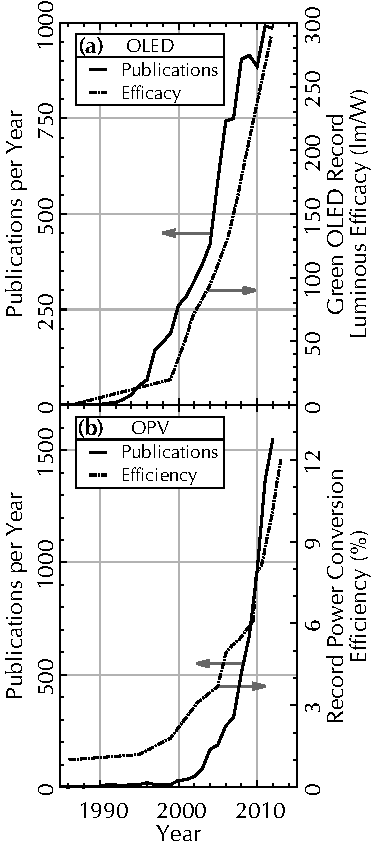
\includegraphics{plot/oled+opv-pub+eff}}
\caption
[OLED and OPV publications per year and laboratory ``hero'' performance]
{(a) OLED and (b) OPV publications per year and laboratory ``hero'' performance.\cite{OW,ISI}
}
\label{fig:oled+opv-pub+eff}
\end{wrapfigure}%
%
%
OLEDs are developed for lighting as well as for display applications.
OLED lighting competes with fluorescent lighting as well as inorganic light-emitting diode (LED) technology.
%
While LEDs are usually point light sources, OLEDs are natural area emitters of diffuse light and allow for new design options like transparent lighting panels. At the time of writing, first products are commercially available.
%
OLEDs for display applications have already proven their potential and successfully emerged into markets where they are competing with conventional liquid crystal display (LCD) technology. Key advantages of OLED displays are higher contrast, potentially low power consumption, smaller thickness and larger viewing angle, mostly enabled by the direct emission of light with the desired color instead of a combination of white backlight and color filters like in LCDs.

Organic semiconductor-based photovoltaics is a promising candidate for providing future electricity supply. Besides silicon-based photovoltaics, it seems to be the only non-concentrated technology with sufficient raw material available for a TW-scale production\cite{Feltrin2008}, required for a significant share of worldwide supply of sustainable electricity.
While for silicon-based photovoltaics the record efficiencies stagnated in recent years and only the production costs could be dramatically reduced, in the last 15 years exponentially increasing OPV record efficiencies have been reported, as shown in \figref{oled+opv-pub+eff}\,(b).
%
At the time of writing, a record power conversion efficiency of 12\,\%\cite{Heliatek12.0} 
is published which is below the record for polycrystalline silicon cells (20.4\,\%)\cite{SolarCellEff41} but already above the value for amorphous silicon (10.1\,\%)\cite{SolarCellEff41}.
In contrast to inorganic cells, the efficiency is stable between room temperature and elevated operating temperature and a better low-light performance is reported \cite{Riede2011,Heliatek12.0}.
%
The major drawback for polycrystalline silicon-based photovoltaic modules is the rather long energy payback time (\eg $\approx 2$ years when installed in Germany\cite{PV-Fakten201303}). Roll-to-roll processing of OPV modules on flexible substrates might allow for a high production throughput and hence, together with low material consumption and low fabrication temperatures, enable short energy payback time and low cost\cite{Anctil2012}.
Furthermore, the narrow absorption bands of organic semiconductors allow for fabrication of color-tunable semi-transparent cells as well as for efficiency-optimized tandem or triple cells\cite{Riede2011,Heliatek12.0}.

Two classes of organic semiconductors are typically distinguished: polymers and small molecules.
Polymers are large molecules consisting of repeating structural units and are typically deposited by wet chemical methods like coating or printing from solution. They show higher charge carrier mobilities than small molecules due to their intra-molecular transport, but chain length dispersity and solvent contamination hamper reproducibility.
Small molecules are compounds of rather low molar mass, often allowing for purification and deposition by thermal evaporation, typically in vacuum. Charge carrier mobilities are usually lower than in polymers and the initial cost for large scale production by vacuum deposition tends to be larger compared to solution processing of polymers. However, the thermal evaporation process allows for freely designable multilayer devices, which is hardly possible for polymers, due to the interaction of solvents with layers already deposited and the lack of orthogonal solvents.

Organic semiconductors can be doped by co-depositing electron donating or accepting atoms or molecules along with the host material. Doping of organic semiconductors has been shown to improve device performance significantly\cite{Walzer2007,LuessemRiedeLeo2013-PSS}, but contrary to conventional semiconductors, the underlying physics is far from being completely understood.
It is the aim of this thesis to contribute to the understanding of the fundamental physics of doping of organic semiconductors by studying the molecular doping in vacuum deposited layers of organic small molecules.

This thesis is structured into nine chapters. Following this introduction, chapter~\ref{chap:Theo} provides the theoretical background and reviews relevant literature for the studies presented in the subsequent chapters. In chapter~\ref{chap:Exp},
the experimental techniques as well as the developed setup are explained in detail. Furthermore, the investigated organic compounds are introduced and their key properties along a draft historical background are summarized.
The presentation of the results starts in chapter~\ref{chap:PaddleWheels} with investigations of the fullerene \CS n-doped by the two novel dopants \CrPd and \WPd of extremely low \IEs and which hence are reactive to air. The degradation induced by air-exposure of doped layers is studied and a regeneration treatment is presented.
In chapter~\ref{chap:AirStables}, \CS is n-doped by air-stable precursor compounds (\aob, \dmbi and \meodmbiI) that form the active dopant compound during deposition. This transformation is investigated more closely for the two novel DMBI derivatives.
Following the studies of n-doping, in chapter~\ref{chap:P-Doping} two amorphous hosts (\meo and \lili) are p-doped by two different dopants (\FS and \CSF) and the influence of the molecular energy levels on the doping is analyzed.
Afterwards, in chapter~\ref{chap:P5} the model system of the polycrystalline host \pen p-doped by the similar-sized dopant \FV is investigated and the data are compared to theoretical predictions for this combination.
Finally, in chapter~\ref{chap:Rech} a model is developed that allows to derive lower limits for the charge carrier mobility, the \nLong as well as the \DopEffLong from conductivity data and furthermore allows to narrow down the energetic position of the \EtLong level when combined with Seebeck data.
Concluding, the findings of this thesis are summarized in chapter~\ref{chap:summary} and directions for future studies are outlined.


\cleardoublepage
% %äöüß
%
\chapter{Fundamentals of Organic Semiconductors}\label{chap:Theo}
\addcontentsline{lof}{chapter}{\thechapter\hspace*{1ex} %
Fundamentals of Organic Semiconductors}

%
\intro{In this chapter, the basics of \SC physics are summarized, as they are required for understanding the results presented in this work. Initially the key properties of conventional (inorganic) \SCs (CSCs) are considered. In a second step, organic \SCs (OSCs) are introduced and differences to conventional \SCs are outlined. Finally, the Seebeck effect is discussed and correlations to \SC properties are derived.
}

\newpage

\section{Conventional Semiconductors}\label{sec:TheoConventionalSemiconductors}
This section introduces the fundamentals of \CSCs, in particular the differences between intrinsic and doped \SCs are highlighted. More detailed information can be found in textbooks\cite{Sze,Thuselt,EnderleinSchenk}.
%
\subsection{Intrinsic Semiconductors}\label{sec:Theo-inorg-Bandstructure}%
A \SC (SC) is called intrinsic if it is pure and free of impurities.
A conventional inorganic \SC material, like silicon (Si) or gallium arsenide (GaAs), consists of covalently bound atoms forming a crystalline lattice structure. The discrete energy levels of a single atom are affected by the interaction of the periodically arranged neighboring atoms and a band structure of allowed and forbidden energy eigenstates for electrons is formed.

The population of electrons in the bands depends on the temperature \T. Semiconductors have the special property that at $\T\rightarrow\K{0}$ every band is either completely occupied or empty. Occupied bands are those lying deepest in energy and the highest occupied band is called valence band, whereas the lowest unoccupied band is called conduction band.
The second important property of \SCs is the presence of a forbidden energetic region between the occupied and the empty bands. As only incompletely filled bands can contribute to transport, at $T\rightarrow\K{0}$ charge transport is impossible (unless the material is illuminated or charges are injected).

\begin{wrapfigure}[7]{r}[6.5mm]{22mm}%
{\vspace*{-1.4em}\includegraphics{draw/egap.pdf}}%
\end{wrapfigure}%
In the following, the lowest allowed energy of the conduction band will be called the \EcLong \Ec and the highest allowed energy of the valence band the \EvLong \Ev. The energetic gap between conduction and valence band and hence the difference between \Ev and \Ec is called bandgap \Egap, being a key property of a \SC and is usually in the range of \SIrange{0.5}{2}{\electronvolt}. At room temperature, the typical \SCs Si and GaAS have bandgaps of $1.12$ and \eV{1.42}\cite{Sze}, respectively.

With increasing temperature, an increasing number of electrons from the valence band reaches the conduction band due to their thermal energy, leaving unoccupied states in the valence band, the so-called holes, behind. Holes can be described in a similar manner to electrons and in the following, the indices ``e'' and ``h'' will are used for addressing parameters of electrons and holes, respectively.
%
The \neLong in the conduction band \ne depends on the density of available states $\dos(E)$ in the conduction band and the occupation probability distribution $f(E,T)$, which accounts for the temperature:
\begin{align}
\ne=\int_{-\infty}^\infty \dos(E) \cdot f(E,T) ~ dE
\label{eq:CCD-basic-integral}
\PUNKT
\intertext{Its energy-resolved derivative is called the differential electron density $\n'(E)$:}
\ne'(E)=\dos(E) \cdot f(E,T)
\label{eq:CCD-basic-integral-diff}
\PUNKT
\end{align}
Electrons are fermions\entdecker[Fermi1926]{Enrico Fermi}{Italian}{1901--1954} and therefore each state can only be occupied by one particle. Hence, the occupation probability $f$ is given by the \fFDLong (compare \figref{sim_Fermi-vs-Boltzmann}\,(a)):
\begin{equation} \label{eq:fFD}
\fFD(E,T) = \frac{1}{1+\exp{\frac{E-\Ef}{\kT}}}
\PUNKT
\end{equation}
Here, \kB is Boltzmann's\entdecker{Ludwig Eduard Boltzmann}{Austrian}{1844--1906} constant and at \T[25] the product $\kT=\meV{25.7}$. %0.025692751856473 eV
\Ef is the electro-chemical potential which is temperature-dependent as well. For $\T\to\K{0}$, the \fFDLong becomes a step function and the occupation probability is zero for all states with an energy above the chemical potential ($f_\text{FD}(E,T)=0$ for $E>\Ef$ at $T\to\K{0}$). The highest occupied energy state at \K{0} is called Fermi \emph{energy}. %$\Ef^0$
At higher temperature, the chemical potential is called Fermi \emph{level} and is temperature-dependent. In the following, only the term Fermi level will be used, since all temperatures discussed are well above \K{0}. The Fermi level is the energy correlated to an occupation probability of $50\,\%$ $(\fFD(\Ef,T)=0.5)$. In case of intrinsic \SCs discussed so far, the value of \Ef is close to the middle of the bandgap, compare \eqnref{EfPosIntrinsic} below.

The \fFDLong can be approximated by the \fBLong for $E-\Ef\gg\kT$
\begin{equation}\label{eq:fB}
\fB(E,T)
  = \exp{-\frac{E-\Ef}{\kT}}
\PUNKT
\end{equation}
\Figref{sim_Fermi-vs-Boltzmann}\,(b) compares the two functions and it can be seen that at $E=\Ef$ the value of $\fB(E)$ is twice the value of $\fFD(E)$. At higher energies the error is strongly decreasing \eg already at $E=\Ef+3\,\kT$, the overestimation is as small as $\approx 5\,\%$. A general expression for the overestimation of $\fFD(E)$ by using $\fB(E)$ can be written as
\begin{equation}
\frac{\fFD(E)}{\fB(E)} - 1 = \exp{-\frac{E-\Ef}{\kT}} = \fB(E)
\KOMMA
\end{equation}
which interestingly is identical to the \fBLong itself.

\cBild[t]
{sim_Fermi-vs-Boltzmann}
{Fermi-Dirac and Boltzmann distribution functions}
{(a) \fFDLong $\fFD(E)$ for the occupation probability at \T[25], \K{0} and \grad{100}. (b) Comparison of Fermi-Dirac $\fFD(E)$ and \fBLong $\fB(E)$ for $\T[25]$ ($\kT=\meV{25.7}$).
} % 25C = 25.7meV

The \dosLong of an intrinsic \CSC is zero in the energy gap between valence and conduction band and non-zero in the bands. Close to the minimum of the conduction band it can be approximated by a square root proportionality to the energy above \Ec\cite{Sze} :
\begin{align} \label{eq:DOS-inorg-prop-sqrt}
 \dos(E) &\propto \sqrt{E-\Ec} & \text{for } E>\Ec \PUNKT
\end{align}
% \Eqnref{CCD-basic-integral} for the charge carrier density \ne can therefore be written
% \begin{equation}
% \ne \propto \int_{\Ec}^\infty \sqrt{E-\Ec} \cdot \fDF(E,T) dE
% \PUNKT
% \end{equation}
Using this \dosLong and the Boltzmann approximation for the \fFDLong \fFD, \eqnref{CCD-basic-integral} can be solved analytically to
\begin{align}
\ne&=\Nc\exp{-\frac{\Ec-\Ef}{\kT}}
\label{eq:ne-InOrg-via-Boltzmann}
\PUNKT
\intertext{Analogously to electrons, the \nhLong \nh in the valence band can be derived, resulting in}
  \nh&=\Nv\exp{-\frac{\Ef-\Ev}{\kT}}
\label{eq:nh-InOrg-via-Boltzmann}
\PUNKT
\end{align}
The prefactors \Nc and \Nv are the so-called effective \dosLong in the conduction and valence band, both being proportional to $(\kT)^{3/2}$ and of the unit \si{\per\centi\meter\cubed}.
%when again using the Boltzmann approximation.

The above equations are only valid in thermal equilibrium and have to be modified if an external bias voltage or illumination is applied to the system. Exemplary, the absorption of a photon would lead to an increase of both, \ne and \nh, making it impossible to describe the system with one Fermi level. Instead, separate quasi-Fermi levels for electrons and holes have to be introduced if thermal relaxation inside the bands is much faster than relaxation from band to band.

In an uncharged and undisturbed intrinsic \SC at a given temperature, the number of electrons in the conduction band equals the number of holes in the valence band (neutrality condition). This density is called the intrinsic charge carrier density \ni
\begin{equation} %\label{eq:NeuralityConditionIntr}
 \ne = \nh = \ni
\PUNKT
\end{equation}
It is important to note that the square of $n_\text{i}$
\begin{equation} \label{eq:LawOfMassAction}
 \ni^2 = \ne \cdot \nh = \Nc\Nv\exp{-\frac{\Egap}{\kT}}
\KOMMA
\end{equation}
is independent of the Fermi level \Ef and can be calculated from \Nv, \Nc, and the bandgap \Egap. Equation~\eqref{LawOfMassAction} is the law of mass action, known from basic chemistry. % http://en.wikipedia.org/wiki/Mass_action_law_(electronics)

\subsection{Doped Semiconductors} \label{sec:TheoDopedSCs}% Doping ?
In order to increase the number of free charge carriers \neh of a \SC, suitable impurities of other elements can be introduced.
In a so-called doped \SC, some of the atoms in the lattice structure are replaced by atoms of a different material, having one valence electron more or one valence electron less than the host element. These impurities are called dopants.

In case of a dopant with one additional valence electron, this electron is only weakly bound inside the lattice of the host material, as no partner for a covalent bond is available. Hence, only little thermal energy is needed for this electron to reach the conduction band and thus to increase the \neLong \ne. Such dopants are called donors or n-dopants as they donate their negatively charged valence electron to the host material.

The same principle works in an analogous manner for dopant atoms that have one valence electron less than the host.
These dopants are called acceptors or p-dopants since a valence electron of the surrounding host atoms is taken and a positively charged hole is created on the host.

Silicon, for example, is typically n-doped using phosphorus (P) as donor or p-doped using boron (B) as acceptor with typical dopant concentrations in the range of a few parts per million (ppm).

In the following, \Nd and \Na are the absolute values of the dopant concentration of donors and acceptors in the host material, usually given in the unit \si{\per\centi\meter\cubed}.
The energy levels of the dopants are located in the bandgap of the host. While the donor level \Ed is near the conduction band (below \Ec), the acceptor level \Ea is near the valence band (above \Ev).

\subsubsection{Ionization of Dopants}
Thermal energy is needed for the ionization of dopants and thus generation of free charges for the conduction or valence band. Two classes of dopants can be distinguished: dopants with either a \emph{deep} or a \emph{shallow} level with respect to the host material. Shallow dopants have an energy level than close to the band edge that thermal energy is sufficient to ionize (most of) them. Deep dopants on the other hand, have energy levels several \kT away from the band edge, so that ionization is less probable.
Generally, the density of ionized donors \Ndi and ionized acceptors \Nai are\cite{Shockley}
\begin{align}
\Ndi &= \Nd \left(
1-
\frac
{1}
{1 + \frac{1}{\gd} \exp{\Ed-\Ef}{\kT}}
\right)
\label{eq:DefNdi}
\\
\Nai &=\Na
\left(
\frac
{1}
{1 + \ga \exp{\Ea-\Ef}{\kT}} \right)
\label{eq:DefNai}
\KOMMA
\end{align}
with \ga and \gd being the ground state degeneracy of the donor and acceptor levels. Typically the degeneracy of these levels is $g=2$ as each level can be occupied by two electrons of opposite spin $(\pm\sfrac{1}{2})$. Additional degeneracy can be introduced by the host material. For Si and GaAs, the valence band is twofold degenerate and thus they have two hole levels each being twofold spin degenerate, leading to a value of $\ga=4$ in these materials.
The temperature regime, where the thermal energy is sufficient to ionize almost all dopants ($\Ndi\approx\Nd$ and $\Nai\approx\Na$) is called the saturation range.
%
The ratio of the \nLong \neh to the density of dopants can be defined as doping efficiency \DopEff (for $\Nd\gg\ni$):
\begin{align}
 \DopEff &= \frac{\ne}{\Nd} \quad \text{or}\quad \DopEff = \frac{\nh}{\Na}
\label{eq:DepEff-inorg}
\PUNKT
\end{align}

The law of mass action ($\ni^2 = \ne \cdot \nh$, \eqnref{LawOfMassAction}) is valid for doped \SCs as well. In contrast to intrinsic SCs, for doped SCs the \neLong in the conduction band \ne does not equal the \nhLong in the valence band \nh. Hence, the neutrality condition for doped SCs has to include the ionized dopants as well:
\begin{align}
\ne + \Nai &= \nh + \Ndi
\label{eq:NeuralityCondition} \\
\begin{split}
\Rightarrow
\Nc\exp{-\frac{\Ec-\Ef}{\kT}}
%
&+
%
\Na
\left(
\frac
{1}
{1 + \ga \exp{\Ea-\Ef}{\kT}} \right)
\\
=
%
\Nv\exp{-\frac{\Ef-\Ev}{\kT}}
&+
%
\Nd \left(
1-
\frac
{1}
{1 + \frac{1}{\gd} \exp{\Ed-\Ef}{\kT}}
\right)
\label{eq:NeuralityConditionLong}
\KOMMA
\end{split}
\end{align}
(Boltzmann approximation used).

If, for example in an n-doped SC, only donors and no acceptors ($\Na=0$, $\Nd>0$) are present, the neutrality condition \eqref{NeuralityCondition} and the law of mass action \eqref{LawOfMassAction} can be used to derive an expression for the \neLong in the condition band \ne\cite{Thuselt}:
\begin{align}
 \ne &= \nh + \Ndi \quad \text{and} \quad \nh = \frac{\ni^2}{\ne} \quad \Rightarrow \quad \ne^2 - \ne \Ndi-\ni^2 = 0 \nonumber \\
 \ne &=\frac{\Ndi}{2} + \sqrt{\left(\frac{\Ndi}{2}\right)^2 + \ni^2}
\PUNKT
\end{align}
This clearly shows the two sources for the \neLong in the conduction band: the excited electrons from the valence band and those from the ionized donors. An analogous trend can be found for acceptor-only doping and \nh.

\subsubsection{Fermi Level Position}\label{sec:FermiLevelPosition}\label{sec:TheoDegenerateDoping}
For an intrinsic \SC, the \EfLong \Ef is located close to the middle of the bandgap:
\begin{equation}
 \Ef = \frac{\Ec+\Ev}{2} + \frac{\kT}{2}\cdot \ln \left(\frac{\Nv}{\Nc}\right)
\PUNKT
\label{eq:EfPosIntrinsic}
\end{equation}
Introducing dopants leads to a shift of \Ef. In case of n-doping, the Fermi level moves towards the conduction band, whereas for p-doping, it moves towards the valence band.
By solving the neutrality condition \eqref{NeuralityConditionLong}, the value of \Ef can be calculated, keeping in mind that all four terms (\ne, \nh, \Ndi, \Nai) depend on \Ef.

In case of shallow dopants or at elevated temperatures, when most dopants are ionized, the position of \Ef is given by:
\begin{align}
 \Ef &= \Ec - \frac{\kT}{2}\cdot \ln \left(\frac{\Nc}{\Nd}\right) & \text{for n-doping} \\
 \Ef &= \Ev + \frac{\kT}{2}\cdot \ln \left(\frac{\Nv}{\Na}\right) & \text{for p-doping}
%\PUNKT hier sieht ein Punkt häßlich aus
\end{align}

\begin{figure}[b]
\centering%
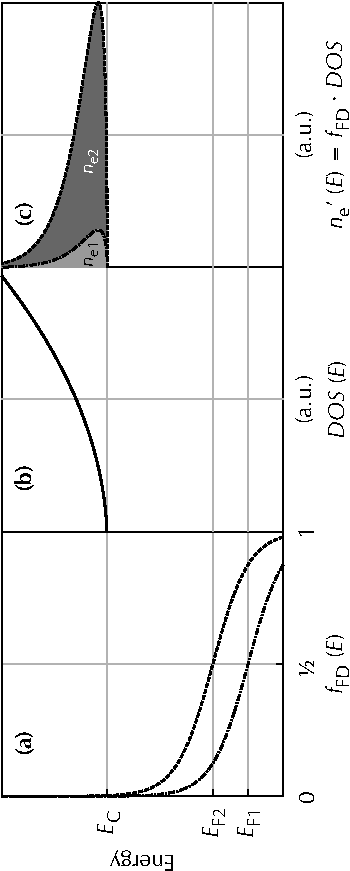
\includegraphics[angle=-90]{plot/sim_Fermi-DOS-n-inorg}%
\setcapwidth[c]{\tmCapWidth}%
\caption
[Influence of \Ef on $\fFD(E)$ and \ne]
{Influence of Fermi level \Ef on \fFDLong $\fFD(E)$ and \neLong \ne for n-doping: (a) $\fFD(E)$ for two different positions of \Ef below the \EcLong \Ec, $\Ef${}$_1=\Ec-\meV{200}$ and $\Ef${}$_2=\Ec-\meV{150}$ (b) \dosLong $\dos(E)$ (c) product of $\fFD(E)$ and $\dos(E)$, displaying the strong influence of \Ef on the \neLong \ne corresponding to the area under the curve.}
\label{fig:sim_Fermi-DOS-n-inorg}
\end{figure}
%
The influence of \Ef on the \fFDLong \fFD and hence on the \neLong \ne, being the integrated product of \fFD and the \dosLong \dos, is displayed in \figref{sim_Fermi-DOS-n-inorg}. It is drawn for the case of n-doping, hence \Ef shifts towards \Ec.
Two \fFDLong{s} with different values of \Ef, corresponding to different doping concentrations, are drawn in part~(a). $\Ef${}$_1$ is chosen to be \meV{200} below \Ec, $\Ef${}$_2$ is \meV{50} larger and hence \meV{150} below \Ec.
In part~(b) of the figure, the \dos is sketched, showing a square root dependency on the energy above the conduction band minimum \Ec, compare \eqnref{DOS-inorg-prop-sqrt}. Finally, the products of \dosLong and the two different Fermi-Dirac distribution functions are drawn in part~(c). These products correspond to the differential \neLong $\ne'(E)$, as shown by \eqnref{CCD-basic-integral-diff}. Therefore, the areas under the curves are the total densities of free electrons $\ne${}$_1$ and $\ne${}$_2$, respectively, compare \eqnrefPage{CCD-basic-integral}.
For the chosen values of $\Ef${}$_1$ and $\Ef${}$_2$, the \neLong $\ne${}$_2$ is 7~times larger than $\ne${}$_1$, which displays the strong influence of the Fermi level position on the \neLong.
An analogous picture can be drawn for p-doping, where \Ef shifts towards the \Ev and increases the \nhLong \nh.

Extremely high doping concentrations result in the Fermi level approaching the band edge. At a difference less than $2\,\kT$, the \SC properties are vanishing and metallic behavior is observed. Furthermore, the Boltzmann approximation for the \fFDLong is not valid for these so-called degenerate \SCs and the equations can only be solved numerically.

\subsection{Charge Carrier Transport}\label{sec:TheoDiffusionCurrent}\label{sec:TheoDriftCurrent}
Free charges (holes in the valence band and electrons in the conduction band) are in constant motion due to their thermal energy. Besides this random thermal movement, an ordered/directed transport is possible under two conditions: Diffusion transport due to a gradient in the \nLong and hence \Ef in the material and drift transport due to the presence of an electrical field. % Both cases are discussed in the following.

% \subsubsection{Diffusion}
Diffusion transport is the thermally driven motion of charges from regions of higher to regions of lower charge carrier concentration. Hence, diffusion transport takes place if a gradient in the \nLong is present in the material.
Fluctuations of the charge carrier concentration can be generated for example by different temperatures in the material (compare \secref{TheoSeePhenomenological}) or by local excess carrier generation.

% \subsubsection{Drift}
Drift transport is the directed motion of charges, driven by the presence of an electric field \EField. Each electron carries one negative elementary electric charge $-e$, whereas a hole (being an unoccupied electron state) carries $+e$.
An electric field leads to a Coulomb%
\entdecker[Coulomb1785a]{Charles Augustin de Coulomb}{French}{1736--1806} 
force accelerating electrons and holes in opposite directions.

The mean drift velocity $v_\text{d}$ of the charges in direction of the force is proportional to the electric field \EField. The proportionality factor of the unit~\si[per=frac]{\centi\meter\squared\per\volt\per\second} is called the mobility \mob and is usually different for electrons and holes:
\begin{align}
 v_\text{d}^\text{e} = \mobe \cdot \EField & & v_\text{d}^\text{h} = \mobh \cdot \EField \label{eq:vdrift}
\PUNKT
\end{align}
In a general case, \eg for non-isotropic materials, the mobility is a tensor and \lasteqn must be read vectorially. The mobility of charges in a \SC depends on many parameters, \eg morphology, \nLong, electric field and temperature. At low temperatures, the mobility is limited by scattering at ionized impurities, due to the low energy and hence low velocity of the charge carriers. Therefore, a decrease in temperature usually leads to a decrease in mobility. At high temperatures on the other hand, the charge carrier motion is disturbed by lattice vibrations, so-called phonons, leading to a decreasing mobility as well. In the temperature region between these two regimes, typically around room temperature, the mobility has a maximum.

% \subsubsection{Conductivity}
As the electric field \EField is defined as the gradient of the electric potential $V$, a field across a material can be generated by applying different electrical potentials to either side of the material.
Applying a voltage~$V$ between two parallel sheet contacts of distance \dc the resulting electric field \EField is
\begin{equation}\label{eq:Efield}
\EField = \frac{dV}{dx} = \frac{V}{\dc}
\PUNKT
\end{equation}

The drift of charges towards the contacts sum up to a current flow $I$ through the material, following Ohm's%
\entdecker[Ohm1827]{Georg Simon Ohm}{German}{1789--1854}
law. In case of a material cross-section $A$, Ohm's law can be written as
\begin{align}
I&=\frac{1}{R}\cdot V = \frac{A \c}{\dc}\cdot V \Rightarrow \c = \frac{I}{V} \cdot \frac{d_\text{c}}{A}
\label{eq:Cond-I-V-geo}
\KOMMA
\end{align}
with the conductivity \c of the material defining its resistance $R=\sfrac{d_\text{c}}{A \, \c}$. The typical unit used for the conductivity of \SCs is $\si{\siemens\per\centi\meter} = \si[per=frac]{\per\ohm\per\centi\meter}$. Applying a voltage~$V$ and measuring the current response $I$, the conductivity of the material can be calculated using \lasteqn.

Instead of the total current $I$, the geometry independent current density $j=\sfrac{I}{A}$ is used to compare different measurements.
The current density can be written as the sum of electron and hole contributions, each being the product of the \nLong and their mean velocity:
\begin{equation}
 j = e \ne v_\text{d}^\text{e} + e \nh v_\text{d}^\text{h}
\PUNKT
\end{equation}
Combining equations \eqref{vdrift}-\lasteq, the conductivity of a \SC can be written as
\begin{equation} \label{eq:Cond-CCD-Mob}
 \c = e \cdot \ne \cdot \mobe  + e \cdot \nh \cdot \mobh
\PUNKT
\end{equation}


%äöüß

\newpage
\section{Organic Semiconductors}\label{sec:TheoOrganicSemiconductors}
In this section, molecular organic \SCs (OSCs) are introduced and the main differences to \CSCs (CSCs) are discussed. For more general properties of \OSCs, the reader is referred to the textbooks~\cite{PopeSwenberg,SchwoererWolf}.

Organic, \ie hydrocarbon-based, chemistry allows for the synthesis of a large variety of molecules. Despite most of the organic molecules being electrical isolators, in the last century semiconducting\cite{Bolto1963}, metallic\cite{Ferraris1973,Coleman1973} and even superconducting\cite{Jerome1980} organic molecules have been discovered.
As shown in \figrefPage{oled+opv-pub+eff}, in recent years, the topic of conducting organic compounds gained more and more attention and in 2000, Heeger, MacDiarmid, and Shirakawa were awarded with the Nobel Prize in chemistry for their work on highly conducting conjugated polymers\cite{NobelChem2000}.
Since this thesis focuses on semiconductor physics, only this class of materials will be discussed in the following.

When atoms form molecules, the atomic orbitals (being solutions to the Schrödinger\entdecker[Schrodinger1926]{Erwin Rudolf Josef Alexander Schrödinger}{Austrian}{1887--1961} %
equation and describing the probability of an electron to be located in a specific spatial region) are combined to molecular orbitals, whereby the number of molecular valence orbitals equaling the total number of atomic valence orbitals prior to the formation of the molecule.
Since electrons are fermions and hence are subject to the Pauli\entdecker[Pauli1925]{Wolfgang Pauli}{Austrian}{1887--1961} exclusion principle, each orbital can only be occupied by two electrons of opposite spin.
Orbitals are populated by electrons according to their energy levels.

\cBildDraw[t]
{molPhys}%
{Formation of hybrid orbitals and delocalized $\pi$-electron-system}%
{%
(a)~Orbitals and bonds for two sp$^2$-hybridised carbon atoms, as in ethylene.
(b)~Delocalized $\pi$-electron-system in a benzene ring consisting of six sp$^2$-hybridised carbon atoms. Images taken from reference\cite{OW} and modified.
}%

Carbon, being the building block of organic molecules, has six electrons: two core electrons and four valence electrons.
The first and second s-orbitals are populated each by two electrons and the remaining two electrons are located in two of three degenerate 2p-orbitals. This configuration is abbreviated as 1s$^2$2s$^2$2p$^2$. Whereas s-orbitals are symmetric around the nucleus, the three 2p-orbitals are dumbbell-shaped\cite{Upper1974}, as drawn in \figref{molPhys}\,(a).
%
Upon formation of molecules, for carbon atoms it is energetically favorable that the valence orbitals rearrange and form hybrid orbitals. Depending on the number of contributing atomic p-orbitals these hybrids are called sp, sp$^2$ or sp$^3$. In case of sp$^2$ configuration, the four valence electrons populate three degenerate hybrid sp$^2$-orbitals and one remaining p-orbital. The sp$^2$-orbitals align in one plane, perpendicular to the remaining p-orbital. Adjacent carbon atoms form covalent $\sigma$-bonds with their hybrid orbitals, which are located between the atoms. The remaining p-orbitals form a second so-called $\pi$-bond parallel to the plane of the sp$^2$-orbitals, as sketched in \figref{molPhys}\,(a).
This $\pi$-bond leads to delocalization of the $\pi$-electrons, which can extend over many atoms, as drawn in \figref{molPhys}\,(b) for the case of six carbon atoms forming a benzene ring. Hence, the electrons in the delocalized $\pi$-system are no longer constrained to single atoms and owing to this delocalization, electron transport through the molecule is significantly improved. Inter-molecular electron transport is enabled via interactions between the $\pi$-systems of adjacent molecules and tunneling of electrons, so-called hopping.
%
For more information on the fundamental physics of molecules, the reader is referred to the textbooks~\cite{HakenWolf,DemtroederExp3}.

The energetic difference between the highest occupied and the lowest unoccupied $\pi$-orbital is smaller compared to the hybrid sp$^2$-orbitals. Thus, in a molecule with delocalized $\pi$-system, the highest occupied molecular orbital (HOMO) and the lowest unoccupied molecular orbital (LUMO) are typically delocalized $\pi$-orbitals.
Since the energetic difference between HOMO and LUMO typically decreases with increasing the delocalization over more atoms, the design of molecules with desired energy levels is possible.
If the energetic difference between HOMO and LUMO is small enough, the molecule can show semiconducting properties.
Consequently, the HOMO level of a molecular semiconductor can roughly be compared to the valence band minimum of a \CSC and analogously the LUMO level to the conduction band minimum.

Organic \SCs can be divided into two major categories: small molecules and polymers.
Semiconducting small molecules include aromatic hydrocarbon compounds like anthracene and pentacene; as well as pyrenes, perylens, oligothiophenes and phtalocyanines. Polymeric \OSCs include aromatic compounds like polythiophenes, polyacetylene and their derivatives.
While layers of small molecular \SCs are usually deposited by thermal evaporation in vacuum, the heavier polymers are commonly processed from solution.
In this work, only thermally deposited small molecules are investigated.

The main difference between OSCs and CSCs is that instead of covalently bound atoms, the molecules interact via the weaker van der Waals%
\entdecker[VanderWaals1873]{Johannes Diderik van der Waals}{Dutch}{1837--1923}
forces. As a result, OSCs are usually amorphous or polycrystalline and have lower dielectric constants in the order of $\varepsilon\approx3$ to 5 compared to CSCs with $\varepsilon\approx10$ to 15\cite{RiedeLuessemLeo2011}. The lower $\varepsilon$ results in a lower shielding of charges and thus to a stronger Coulomb interaction between them, compared to CSCs.

One advantage of the weak van der Waals interaction between the molecules and the disordered structure of OSCs is that they are less sensitive to impurities and structural defects than CSCs. They can inherit impurity levels of up to a fraction of percent and still work well\cite{RiedeLuessemLeo2011}, whereas such high concentrations would render CSCs completely useless. As a consequence, intentional doping concentrations have to be considerably higher for OSCs, which is discussed in \secref{TheoDopingOrg}.

\subsection{Charge Carrier Transport}
Due to the weak inter-molecular interaction, non-crystalline OSCs usually do not form a band structure of allowed and forbidden energy regions (compare \secref{Theo-inorg-Bandstructure}). Instead, the charge transport occurs via hopping processes from one molecule to the other.
One characteristic attribute for hopping transport is its temperature dependence. While for CSCs the mobility decreases at elevated temperatures due to scattering of the charges at lattice vibrations (compare \secref{TheoDriftCurrent}), for OSCs the hopping probability and hence the mobility increase with temperature. Usually, the conductivity \c is found to be thermally activated as
\begin{equation}\label{eq:CondActivation}
\c(T) = \c_0 \exp{-\frac{\Eact}{\kT}}
\KOMMA
\end{equation}
where \kB is Boltzmann's constant, $\c_0$ is interpreted as theoretical maximum of the conductivity and \Eact is the \EactLong.

The temperature dependence of the mobility may differ from a simple activated case to a model where hopping along a manifold of states is assumed\cite{Bassler1982, Vissenberg1998}. Besides the temperature, the mobility is influenced by the \nLong and applied external fields as well, but this interaction is not completely understood at present. For further information on charge transport in organic molecules, the reader is referred to the review articles~\cite{Tessler2009,Troisi2011}. An overview about traps in \OSCs is given in reference\cite{Schmechel2004}.

\subsection{Density of States}\label{sec:TheoOrgDOS}
%
\cBild{sim_gauss-malen}%
{Normalized Gaussian distributed \dosLong}%
{Sketch of a normalized Gaussian distributed \dosLong, following \eqnref{DefGaussianDOS} and arbitrary positioned at \mbox{$\gausscenter=0$}.}%
%
The \dosLong of \OSCs has a different distribution than for \CSCs. While for CSCs a square root shaped \dos can be approximated near the band edges, compare \secref{TheoConventionalSemiconductors}, for OSCs usually a Gaussian\entdecker{Johann Carl Friedrich Gauß}{German}{1777--1855} distribution is assumed \cite{Schmechel2003, Tietze2012}, which accounts for the energetic broadening of molecular energy levels due to the disorder as well as intra- and inter-molecular interactions and orientations.
The \dos of OSCs can be modeled by the following equation, which is drawn in \figref{sim_gauss-malen}:
\begin{equation} \label{eq:DefGaussianDOS}
\dos(E) = \frac{\nH}{\sqrt{2 \pi} ~ \gausswidth} \exp{-\frac{(E-\gausscenter)^2}{2\gausswidth^2}}
\PUNKT
\end{equation}
Here, \gausscenter is the position of the maximum of the distribution and \gausswidth is the standard deviation, being a measure for the width of the Gaussian distribution. At \mbox{$E=\gausscenter\pm\sqrt{2}~\gausswidth$} the distribution is reduced to the maximum divided by Euler's\entdecker{Leonhard Euler}{Swiss}{1707--1783} number. As each molecule is assumed to be able to contribute one state, integration of $\dos(E)$ over all energies yields the total density of (host) molecules \nH.

Similar to a square root shaped \dosLong, for a Gaussian shaped \dos it is possible to solve \eqnrefPage{CCD-basic-integral} for the \nLong \neh analytically, when using the Boltzmann approximation for the \fFDLong\cite{Tietze2012}. For clarity, additional steps not included in the original publication are shown here, as well as the adoption of this approach for electrons instead of holes:
\begin{align}
\ne &=\int_{-\infty}^{+\infty}
 \overbrace{ \frac{\nH}{\sqrt{2 \pi} ~ \gausswidth} \exp{-\frac{(E-\gausscenter)^2}{2\gausswidth^2}} }^{\dos(E)}
 ~ \cdot ~
 \overbrace{ \exp{-\frac{E-\Ef}{\kT}} } ^{\fB(E)}
 dE
% \KOMMA hier nicht
\\
\intertext{
with $x:=E-\gausscenter$ , $C_1:=\frac{\nH}{\sqrt{2 \pi} \gausswidth}$ and $C_2 := \frac{\gausswidth^2}{\kT}$ this becomes
}
\ne &= C_1 \int_{-\infty}^{+\infty} dx
 \exp{-\frac{1}{2\gausswidth^2}
   \left(
     x^2 + 2 x C_2 + 2 C_2 \left( \gausscenter-\Ef \right)
   \right)
 }
\\
\intertext {
  with $\left( x + C_2 \right)^2 = x^2 + 2xC_2 + C_2^2 $ this simplifies to
}
\ne &= C_1 \int_{-\infty}^{+\infty} dx
 \exp{-\frac{1}{2\gausswidth^2}
   \left(
     \left( x + C_2 \right)^2 - C_2^2 + 2 C_2 \left( \gausscenter-\Ef \right)
   \right)
 }
\\
&= C_1
\exp{-\frac{- C_2^2 + 2 C_2 \left( \gausscenter-\Ef \right)}{2\gausswidth^2} }
 \int_{-\infty}^{+\infty} dx
 \exp{-\frac{( x + C_2 )^2}{2\gausswidth^2}
 }
\\
%&= C_1
%\exp{+\frac{C_2^2}{2\gausswidth^2} - \frac{2 C_2 \left( \gausscenter-\Ef \right)}{2\gausswidth^2} }
% \int_{-\infty}^{+\infty} dx
% \exp{-\frac{( x + C_2 )^2}{2\gausswidth^2}
% }
%\\
&= C_1
  \exp{+\frac{\gausswidth^2}{2(\kT)^2} - \frac{ \gausscenter-\Ef }{\kT} }
    \int_{-\infty}^{+\infty} dx
    \underbrace{
      \exp{-\frac{\left( x + \frac{\gausswidth^2}{\kT} \right)^2}{2\gausswidth^2}
      }
    } _ { \text{= definition of Gaussian, compare \eqref{DefGaussianDOS}}}
\\
&= \nH\frac{1}{\sqrt{2 \pi} \gausswidth}
  \exp{+\frac{\gausswidth^2}{2(\kT)^2} - \frac{ \gausscenter-\Ef }{\kT} } \quad \cdot \sqrt{2\pi}~\gausswidth
\\
\ne &= \nH
  \exp{-\frac{ \left(\gausscenter - \frac{\gausswidth^2}{2\kT} \right) -\Ef }{\kT} } \label{eq:ne-org-solved} 
\PUNKT
\intertext{An analogous calculation\cite{Mayer2010} can be performed for p-doping to obtain the \nhLong \nh, when a corresponding \dosLong is used, (having its maximum below \Ef)} \nh &= \nH
  \exp{-\frac{ \Ef - \left(\gausscenter + \frac{\gausswidth^2}{2\kT}\right)}{\kT}}
\label{eq:nh-org-solved}
\PUNKT
\end{align}
These terms are similar to the equations for CSCs:
\begin{align*}
\ne &=\Nc\exp{-\frac{\Ec-\Ef}{\kT}} \quad\quad\text{\eqref{ne-InOrg-via-Boltzmann}}&  \nh &=\Nv\exp{-\frac{\Ef-\Ev}{\kT}} \tag{\ref{eq:nh-InOrg-via-Boltzmann}}
\PUNKT
\end{align*}
In case of a Gaussian distributed \dosLong, the prefactors \Nc and \Nv are replaced by the density of molecules \nH and the energy level of the conduction band is replaced by a term that depends on the position of the maximum \gausscenter and the width \gausswidth of the Gaussian distribution.

If \Ef is close to \gausscenter and hence \fB is strongly overlapping with the \dosLong, the Boltzmann approximation is not valid. Here, the \fFDLong $\fFD(E)$ has to be used and the integral \eqref{CCD-basic-integral} solved numerically. Both functions, \fFD and \fB, are drawn in \figref{sim_Fermi-DOS-Es-org-Fermi-vs-Boltzmann} together with a Gaussian \dos, where \Ef is arbitrary placed at a distance of $4 \cdot \gausswidth$ from the \gausscenter. The product of distribution function and \dos is the differential \neLong $\ne'(E)$ and is shown as inset. The area under that curve corresponds to \neLong \ne, analogously to \figrefPage{sim_Fermi-DOS-n-inorg}. It can clearly be seen that using \fB, \ne would be overestimated as the contribution for $E<\Ef$ is strongly overrated. Therefore, in the following all calculations of \neh are performed numerically, using \fFD.

\cBild
{sim_Fermi-DOS-Es-org-Fermi-vs-Boltzmann}
{Overestimation of \ne by using \fB instead of \fFD in a Gaussian \dos}
{Comparing the influence of Boltzmann \fB and Fermi-Dirac \fFD distribution functions on the \neLong \ne for the case of \Ef close to \gausscenter, here at a distance of $4\,\gausswidth$. Inset: product of \dos and $f$, being the differential \neLong $\ne'(E)$, calculated for \fFD (light gray) and overestimation via \fB (dark gray). Parameters: \mbox{$\gausswidth=\meV{100}$}, \mbox{$\Ef=Eg-4 \cdot \gausswidth$}, \T[25].
}

\subsection{Doping of Organic Semiconductors}\label{sec:TheoDopingOrg}
Doping of \CSCs was the key element that led to the breakthrough of semiconductor technology, as it allows for control of the majority charge carriers and hence the design of p-n-junctions, the building block for most modern electronic devices. Furthermore, doping allows for adjusting the conductivity as well as the position of the \EfLong position in a layer, enhancing device design freedom and performance.
Similar to \CSCs, it is possible to dope \OSCs by adding electron acceptors or electron donors to the layer, which drastically increases the \nLong.
Hence, doping of \OSCs raises the \cLong by several orders of magnitude and furthermore allows to overcome contact limitations between metal contacts and organic layers and thus improves charge injection and extraction, which are crucial for efficient devices. Besides increasing the \nLong, doping can also effect the charge carrier mobility by either filling of traps or by generation of additional traps\cite{Schmechel2004,Arkhipov2005}.
In the following, a brief overview about history and different approaches for doping of organic layers is given. For more details, the reader is referred to the textbook chapters~\cite{RiedeLuessemLeo2011,LuessemRiedeLeo2012,HummertLeo2013} and the review articles~\cite{Walzer2007,LuessemRiedeLeo2013-PSS}.

\subsubsection{History of Doping Experiments}
First attempts of p-doping of \OSCs have been reported as early as 1954 when Akamatu\etal\cite{Akamatu1954} used the halogen bromine as acceptor in perylenes. Later, extensive studies on p-doping using halogen gases have been performed\cite{Curry1962,Yamamoto1979}. 
Oxygen-exposure can lead to p-doping as well\cite{Vaterlein1996,Hamed1993}.
Successful n-doping has first been reported\cite{Ramsey1990,Haddon1991} in 1990, when alkali metals like cesium % BE: Caesium, AE: Cesium
were used as donors and have recently been theoretically described\cite{Mityashin2012}.

A common problem of using atoms to dope an OSC is the diffusion of atoms through the device that leads to a lowering of device efficiency and lifetimes\cite{Walzer2007}. This issue can be overcome by using larger or heavier compounds, like organic molecules. A molecular n-dopant donates an electron from its HOMO to the LUMO of the host material, whereas a molecular p-dopant accepts an electron from the HOMO of the host into its LUMO, creating a hole at the host. Thus, for successful doping suitable energy levels of host and dopant are required. 

The first successful p-doping of an OSC using an organic dopant has been shown by Kearns\etal\cite{Kearns1960} in 1960. Molecular p-dopants are strong electron accepting molecules with a deep lying LUMO level. They typically contain fluorine, the most electronegative element in the periodic table.
In recent years, heavy metal oxides like MoO$_3$ or WO$_3$ have gained attention as these molecules have been reported to be less diffusive\cite{Chang2006} and are able to dope materials with HOMO levels as deep as \eV{6}\cite{Meyer2009,Kroger2009}.

It took 40 more years until the first organic n-dopant has been reported by Nollau\etal\cite{Nollau2000} in 2000. The reason is that n-dopants need to have shallow HOMO levels (with respect to the vacuum level) in order to donate an electron into the LUMO of the host. Therefore, they are highly reactive materials that are usually unstable in air and hence require handling in an inert atmosphere.

The n-dopants reactivity to air can be alleviated by using stable precursor compounds which form the active dopant compound \insitu during depositing of the doped layer in vacuum. This approach has been first presented by Werner\etal\cite{Werner2003} using the cationic salt % cation = pos charged dopant
pyronin B chloride which upon vacuum deposition separates from its chloride anion. Recently, a different approach has been presented by Guo\etal\cite{Guo2012}, who used dimers that were cleaved during deposition, yielding the advantage of less unintended side products that could interfere with the doping process.

\subsubsection{Doping Mechanisms}\label{sec:Theo-org-Doping-Mechanisms}
Doping is usually described as a two-step process. First, the dopant is ionized, transferring an electron (or hole) to the host and leaving a hole (electron) on the dopant molecule behind. Afterwards, the electron (hole) has to dissociate against the Coulomb attraction of the hole (electron) left on the dopant. This principle holds for conventional and organic \SCs.

In case of molecular doping of an organic host, a suitable dopant molecule is required for the first step.
The \IE (IE) corresponds to the difference between the HOMO and the vacuum level, compare \figref{Skizze-Doping-org}\,(a), and is a measure of the energy it takes to remove the least bound electron from the molecule.
On the other hand, the difference between the LUMO and the vacuum level is referred to as \EA (EA).
A molecule with a low IE is likely to donate electrons and can therefore be used as n-dopant, whereas p-dopants typically have high EA to allow for electron accepting, as sketched in \figref{Skizze-Doping-org}\,(b) and (c).
The IE can be measured using ultraviolet photoelectron spectroscopy (UPS) in vacuum with a typical accuracy of $\pm\eV{0.13}$\cite{SelinaOlthofDiss}. The EA on the other hand can be studied by inverse photoemission spectroscopy (IPES) in vacuum, which due to a smaller cross-section has a lower accuracy, typically around $\pm\eV{0.30}$. Recently, a high resolution IPES setup has been presented\cite{Yoshida2012} that uses electrons of kinetic energies below \eV{4} and is a promising method for measuring the EA with higher accuracy.
Soluble compounds can be probed by the wet chemical method of cyclic voltammetry (CV), which allows for an estimation of HOMO and LUMO levels, but as the energy levels usually differ between solutions and deposited layers, for the samples investigated in this thesis, values determined by UPS and IPES are preferred.
%
As it is difficult to measure the molecular energy levels of dopants deposited into a layer of host molecules, today it is not clear if the energy levels of the dopants are affected by the surrounding host molecules. Therefore, in this work the energy levels of dopant molecules deposited into layers of hosts molecules are assumed to remain at the levels determined for pure dopant layers.
%
Besides suitable energy levels, overlap of orbitals between host and dopant, as well as morphological properties are essential for charge-transfer.

%
\cBildDraw[t]
{Skizze-Doping-org}
{Sketch of doping principle for OSCs}
{Sketch of doping principle for OSCs. (a) Relation of HOMO and LUMO to vacuum level via \IE (IE) and \EA (EA). (b) n-doping: an electron is transfered from the HOMO of the dopant to the LUMO of the host. (c) p-doping: an electron is transfered from the HOMO of the host to the LUMO of the dopant, generating a hole at the host.
}

The second step of doping, the dissociation of the generated charge pair, is easier to achieve for CSCs, as their dielectric constants ($\varepsilon\approx10$ to 15) are higher than for OSCs ($\varepsilon\approx3$ to 5)\cite{RiedeLuessemLeo2011}. Therefore, the Coulomb interaction between charges is much stronger in case of OSCs, requiring a larger distance between the charges to overcome the attraction.

Mityashin\etal\cite{Mityashin2012a} calculated the potential landscape around an ionized dopant for the model system of \pen doped by \FV\footnote{compare \secref{Mat} for details on the materials}, as these molecules have a similar size as well as suitable energy levels. Varying the concentration of dopants in the system, they found that a certain minimum concentration of dopants is required in order to change the potential landscape sufficiently to allow for dissociation and hence generation of free charges. This finding is different to CSCs, where no fundamental lower limit of doping concentration is known.
Their results explain the much higher doping concentrations needed for OSCs, compared to CSCs.

Salzmann\etal\cite{Salzmann2012} introduced an alternative model for the doping process of OSCs, suggesting the formation of a hybrid of host and dopant by a hybridization of their orbitals. They conclude that due to an offset of the energy levels of host and hybrid state, only a fraction of the hybrids can be ionized at finite temperature and thus the maximum \nLong is limited.

\subsubsection{Units of Doping Concentration}\label{sec:TheoDopingUnits}
While in CSCs typically doping concentrations are in the part per million (ppm) range, for OSCs much higher concentrations, typically in the range of several percent are required. The reasons are the disordered structure that leads to the lower charge carrier mobilities and the high density of traps, which has to be overcome by doping, as well as the above discussed required change in potential landscape.
In OSCs, the \CLong \C is usually expressed either in terms of weight (\eg \wt{}) or in terms of molecule numbers (\eg mol\%). Using terms of weight is more technically oriented, as during sample fabrication typically the weight of the materials is directly controlled. Expressing \C in terms of numbers of molecules, on the other hand, is physically easier to interpret but requires the knowledge of the molar mass \MM of each compound, which for proprietary materials or compounds that transform during deposition may not be available. As the structures of all materials used in this thesis are known, the \CLong can be expressed in terms of numbers of molecules.
Thereby, it is assumed that the dopant molecules substitute host molecules and therefore adopt the density of the host. The unit molar ratio (\mr{}), being the ratio of dopant to host molecules, is a relevant figure for quantitative evaluations and hence chosen as unit for all \CLongs in the following:
\begin{align}
\C \text{ in } \mr{} &= \frac{\nD}{\nH}
\KOMMA
\intertext{with \nHLong \nH and \nDLong \nD. Besides \mr{}, in literature frequently the unit molar percent (mol\%) is found, being defined as the relative number/density of dopant molecules to the total number/density of molecules}
\text{mol}\% &= 100\% \cdot \frac{\nD}{\nH+\nD}
\PUNKT
\intertext{Analogously to mol\%, the unit weight percent (\wt{}) is defined as ratio of the mass of dopant material to the total mass}
\wt{} &= 100\% \cdot \frac{m_\text{D}}{m_\text{H}+m_\text{D}}
\PUNKT
\end{align}
Conversion between the different units can be performed via
\begin{align}
\mr{} &= \frac{\text{mol}\%}{100\%-\text{mol}\%}
&% \quad \text{and} \quad
\text{mol}\% &= 100\% \cdot \frac{\mr{}}{\mr{}+1}
\\
\mr{} &= \frac{\MM{}_\text{H}}{\MM{}_\text{D}} \cdot \frac{\wt{}}{100\%-\wt{}}
&% \quad \text{and} \quad
\wt{} &= 100\%\cdot \left(1+\frac{\MM{}_\text{H}}{\MM{}_\text{D}}\cdot\frac{1}{\mr{}}\right)^{-1}
\label{eq:MRtoWT}
% \KOMMA
\end{align}
with the molar masses of host and dopant, $\MM{}_\text{H}$ and $\MM{}_\text{D}$, respectively.

\subsubsection{Calculating Molecular Densities}
In an undoped layer, the density of molecules \nM can be calculated from the molar mass \MM and the density \density of the material, using the Avogadro\entdecker{Lorenzo Romano Amedeo Carlo Avogadro, Conte di Quaregna e Cerreto}{Italian}{1776--1856} constant \avogadro:
\begin{equation}
 \nM = \frac{\avogadro \cdot \density}{\MM}
\label{eq:nM-from-MatPara}
\PUNKT
\end{equation}
In a doped layer, \nM is the sum of partial densities of host \nH and dopant \nD molecules. Assuming dopant molecules to neatly replace host molecules one by one, the total density of molecules \nM is unchanged upon doping. Expressing the doping concentration \C in terms of molar ratio \mr{}, the following expressions for \nH and \nD can be derived:
% , which are plotted in \figref{sim_H+D-vs-MR}:
\begin{align}
 \nM &= \nH + \nD \label{eq:nMHD}\\
 \C  &= \frac{\nD}{\nH}\label{eq:C} \\
% \nD &= \C \cdot \nH  \\
 \nH = \frac{\nM}{1+\C}
 \quad \quad &\text{and} \quad \quad
 \nD = \frac{\nM\cdot\C}{1+\C}
\label{eq:nHD}
\PUNKT\\
%\end{align}
\intertext{%
For dopant densities much greater than the intrinsic charge carrier density \ni, the doping efficiency \DopEff is defined as the ratio of the density of free charge carriers (electrons or holes) \neh to the \nDLong \nD, analogously to \eqnref{DepEff-inorg} for CSCs:}
%\begin{align}
\DopEff &= \frac{\neh}{\nD} = \neh \cdot \frac{1+\C}{\nM\cdot\C}
\label{eq:DopEff}
% = \frac{\neh}{\C \cdot \nH}
\\
\Rightarrow \neh &= %\DopEff \cdot \nD = \DopEff \cdot \C \cdot \nH %\\
%= \frac{\neh \cdot (1+\C)}{\C \cdot \nM}
%&= \frac{\neh}{\nM} \cdot \frac{1+\C}{\C}
\DopEff \cdot \nM \cdot \frac{\C}{1+\C}
\label{eq:CCD-from-DopEff}
\PUNKT
\end{align}


%äöüß
\newpage
\section{Seebeck Effect}
The Seebeck effect is of great interest for semiconductor physics, as it allows for determination of the type of the majority charge carriers as well as the relative position of the \EfLong with respect to the \EtLong.

%
\subsection{Phenomenological Description}%
\label{sec:TheoSeePhenomenological}
%\was{discovery, earth mag field}
In 1821, the Estonian-German physicist \name{Thomas Johann Seebeck} discovered\cite{Seebeck1823} that a magnetic force arises when junctions of two different metal wires are heated to different temperatures. He detected the force by a compass needle and therefore named his finding the \emph{thermomagnetic} effect.
Seebeck interpreted this effect to be the origin of the earth's magnetic field, due to the veins of metals and ores in the ground\cite{Seebeck1823}.
Nowadays we know that his conclusion is wrong since the earth's magnetic field is explained by the motion of molten iron alloys in the earth's core. Furthermore, today it is proven that in Seebeck's discovery not a magnetic force is generated in the first place, but a voltage gradient that drives charges along the wires, which leads to the magnetic field he detected. Hence, his discovery is now called \emph{thermoelectric} or Seebeck effect.
%\was{metals and semiconductors, but not supercond.}
This effect is observed for both, metals and semiconductors, but not for superconducting materials (at temperatures below their critical temperature), as a resistance free material cannot hold a voltage gradient.

%\was{origin of S}
Phenomenologically, the Seebeck effect can be understood as follows: In a metal or semiconductor, the energetic distribution of the free charge carriers is shifted to higher energy states upon heating (compare \secref{TheoConventionalSemiconductors}). Thus, if one side of the material is hotter than the other, the charge carriers on the hotter side have higher energies on average.
This leads to a displacement diffusion current (compare \secref{TheoDiffusionCurrent}) towards the cold side, resulting in a charging of the two sides of the material. With increasing charge accumulation at the sides, an electric field opposite to the diffusion current builds up, limiting the total voltage being generated.
If electrons are the dominating charge carriers, the cold side will be charged negatively, whereas for hole dominated materials the cold side is charged positively. Therefore, the Seebeck effect can be used to identify the type of dominating charge carriers in the material.

%\subsection{Applications}
Different devices employ the Seebeck effect. Examples are a prominent class of thermometers, the thermocouples (used in our setup to measure the temperatures of the material sources, as discussed in \secref{ExpTechDetails}), as well as thermoelectric generators, which generate electricity from temperature gradients.
% Thermoelectric generators are used to harvest waste heat of engines to supply independent small devices.
Future applications in space flight might be possible, as the large temperature difference between space and the inside of the shuttle are beneficial for this kind of power supply. Recently, Kraemer\etal published\cite{Kraemer2011} a design for a solar driven thermoelectric generator as alternative to photovoltaic cells with a peak efficiency of \SI{4.6}{\percent}. % under illumination conditions of AM1.5G
Requirements for materials for thermoelectric generators are a strong Seebeck effect and high electrical conductivity combined with low thermal conductivity.
Insects utilize the Seebeck effect is as well: The cuticle of hornets for example, has been reported\cite{Shimony1981,Barron2009} to show positive and negative values, for the yellow-colored and brown-colored cuticle, respectively. It is speculated that the hornets use this for temperature detection.
Recently, the spin Seebeck effect has been reported, which should allow for spin-voltage generators, being crucial for driving spintronic devices\cite{Uchida2008}.

\subsection{Definition and Measurement of the Seebeck Coefficient}\label{sec:TheoSeeDefAndMeas}
If two sides of a material are held at different temperatures, a voltage \V is generated, which is proportional to the temperature difference $\Delta T$ for small $\Delta T$. The proportionality is given by a material property called Seebeck coefficient \S, which is defined for spatial steps of infinitesimally small temperature differences along the material, as
\begin{equation}
 \S(\Tm) := \lim_{\Delta T\to0} \frac{\Delta \V}{\Delta T}
\label{eq:DefSeebeck}
 \PUNKT
\end{equation}
The total voltage difference \Vs between the ends of the material is given by the path integral along the material\cite{WagnerDiss2007}:
\begin{equation}
\Vs = \int_{x_1}^{x_2} S(T) ~ \partial_x T ~ dx
= \int_{T_1}^{T_2} S(T) ~ \partial_x T ~ dT
\label{eq:DefVs}%TheoVs
\PUNKT
\end{equation}
Choosing $T_2-T_1$ to be small enough that the Seebeck coefficient $S(T)$ can be considered constant in the range of $T_1$ to $T_2$ and additionally assuming a linear temperature gradient, \lasteqn can be simplified to
\begin{equation}
\Vs = \S \int_{T_1}^{T_2} ~ \partial_x T ~ dT = \S \cdot (T_2-T_1)
\PUNKT
\end{equation}
In general, the Seebeck coefficient is temperature-dependent and will therefore be written as $\S(\Tm)$ in the following, with \Tm being the mean temperature of $T_1$ and $T_2$ and the applied temperature difference is $\Td=T_2-T_1$.

\begin{wrapfigure}[4]{r}[0mm]{21mm}%
{\vspace*{-1.5em}\includegraphics{draw/Seebeck-Zuleitungskizze.pdf}}%
\end{wrapfigure}%
%\was{Measuring, neglecting metal wires}
In order to measure the thermoelectric voltage \Vs along a material A (with a Seebeck coefficient $S_\text{A}$), two points with temperatures $T_1$ and $T_2$ have to be connected by wires of a material B (with Seebeck coefficient $S_\text{B}$) to a voltmeter that is at a temperature $T_3$. It is conventional to contact the \emph{high} input of the voltmeter to the \emph{cold} side. Consequently, a positive sign of the voltage is obtained if holes are the dominating charge carriers.
The total measured thermoelectric voltage is the sum of the individual contributions:
\begin{align}
\Vs &= S_\text{B} \cdot (T_3-T_1) + S_\text{A} \cdot (T_1-T_2) + S_\text{B} \cdot (T_2-T_3) \nonumber\\
&= (S_\text{A}-S_\text{B}) \cdot (T_1-T_2)
\KOMMA
\end{align}
which is independent of the temperature $T_3$ at the voltmeter, but affected by the Seebeck coefficients of the connecting wires $S_\text{B}$.

The Seebeck coefficients of semiconductors are in the range of several hundred to thousand \si{\micro\volt\per\kelvin}, whereas for metals only few \si{\micro\volt\per\kelvin} are measured ($\S{}_\text{SC}\gg\S{}_\text{metal}$). Copper, for example, has $\S\approx\uVK{2}$ at room temperature\cite{DemtroederExp2}. %\cite{Kasap}
Hence, if a metal is used to contact a voltmeter to the ends of an investigated semiconductor, the contribution of the wires in \lasteqn can be neglected and the Seebeck coefficient is
\begin{equation}
% \Vs\approx S_\text{A}\cdot (T_1-T_2) \Rightarrow S_\text{A} = \frac{\Vs}{T_1-T_2}
S_\text{A} \approx \frac{\Vs}{T_1-T_2}
\label{eq:SeebeckMeasured}
\PUNKT
\end{equation}

%\newpage
\subsection{Correlation to Semiconductor Energy Levels}
\subsubsection{Conventional Semiconductors}%
\label{sec:TheoFritzsche}
In 1971 Fritzsche published a correlation of the Seebeck coefficient and the energy levels of a semiconductor\cite{Fritzsche1971}. He started with the Peltier\entdecker[Peltier1834]{Jean Charles Athanase Peltier}{French}{1785--1845}
coefficient \peltier, which correlates to the Seebeck coefficient via the Thomson\entdecker{William Thomson, later 1$^\text{st}$ Lord Kelvin}{British}{1824--1907}
relation
\begin{equation}
\peltier = \S \cdot T
\label{eq:PeltierSeebeck}
\PUNKT
\end{equation}
\peltier, on the other hand, is defined as the energy carried by the electrons per unit charge, whereas the energy is measured with respect to the \EfLong \Ef. The contribution of each electron to \peltier is proportional to its relative contribution to the total conductivity, so \peltier can be written as\cite{Fritzsche1971}
\begin{equation}
\peltier = - \frac{1}{e} ~ \int_{-\infty} ^{+\infty} (E-\Ef) ~ \frac{\c'(E)}{\c} ~ dE
\label{eq:PeltierIntegral}
\KOMMA
\end{equation}
with the differential conductivity $\c'(E)$ that can be defined by equations~\eqref{Cond-CCD-Mob} and \eqref{CCD-basic-integral-diff}, introducing the energetic distribution of the mobility $\mob(E)$:
\begin{equation}
 \c'(E) dE = e \cdot n'(E) \cdot \mob(E) ~dE = e \cdot \dos(E) \cdot \fFD(E) \cdot \mob(E) ~dE
\label{eq:DiffCond}
\PUNKT
\end{equation}
Integration gives the total conductivity
\begin{equation}
 \c(E) = \int_{-\infty} ^{+\infty} \c'(E) dE
\PUNKT
\end{equation}
Using \eqnref{PeltierSeebeck}, the Seebeck coefficient can be written as
\begin{equation}\label{eq:SeebeckIntFritzsche}
\S = \frac{\peltier}{T}=  - \frac{\kB}{e} ~ \int_{-\infty} ^{+\infty} \frac{E-\Ef}{\kT} \cdot \frac{\c'(E)}{\c} ~ dE
\PUNKT
\end{equation}

Fritzsche found that in case of one band only conduction with no states below the conduction band edge \Ec (electron (e) conduction) or above the valence band edge \Ev (hole (h) conduction), \eqnref{SeebeckIntFritzsche} can be simplified to
\begin{align}
\S &= -\frac{\kB}{e} \left( \frac{\Ec-\Ef}{\kT} + A_\text{C}\right) & \text{for e-conduction} \label{eq:Fritzsche-e} \\
\S &= +\frac{\kB}{e} \left( \frac{\Ef-\Ev}{\kT} + A_\text{V}\right) \PUNKT & \text{for h-conduction} \label{eq:Fritzsche-h}
\end{align}
The terms $A_\text{C}$ and $A_\text{V}$ in the order of 1 account for the energetic dependency of the \dosLong $\dos(E)$ and the mobility $\mob(E)$ above \Ec or below \Ev.
If the \EfLong is at a large distance to the corresponding band edge
(\mbox{$\Ec-\Ef\gg\kT$} or \mbox{$\Ef-\Ev\gg\kT$}), $A_\text{C}$ and $A_\text{V}$ can be neglected. This leads to a simplified version of the equations above:
\begin{align}
\S &= - \frac{\Ec-\Ef}{e\,\T} & \quad\quad\text{for e-conduction} \label{eq:Fritzsche-e-ohneA} \\
\S &= + \frac{\Ef-\Ev}{e\,\T} \PUNKT & \quad\quad\text{for h-conduction} \label{eq:Fritzsche-h-ohneA}
\end{align}
%
%
In conclusion, the sign of the Seebeck coefficient \S identifies whether electrons or holes are the dominating charge carriers, whereas the value of \S is correlated to the difference between the \EfLong and the corresponding band edge, \Ec or \Ev. In the following, the term \EsLong \Es will be used for this difference, which has a negative value for electron conduction and a positive value for hole conduction:
\begin{align}
\Es := \Ef-\Ec \quad\text{ or }\quad \Es := \Ef-\Ev
\label{eq:DefEs-Ec-Ev-inorg}
\PUNKT
\end{align}
Equations \eqref{Fritzsche-e-ohneA} and \eqref{Fritzsche-h-ohneA} can hence be simplified to
% For large \Es, the terms $A_\text{C}$ and $A_\text{V}$ in equations \eqref{Fritzsche-e} and \eqref{Fritzsche-h} can be neglected, thus equations \eqref{Fritzsche-e-ohneA} and \eqref{Fritzsche-h-ohneA} are valid and can be simplified to
\begin{align}
\S =& \frac{\Es}{e\,\T} \quad \Rightarrow \quad \Es = \S \cdot e \cdot \T \label{eq:S-Es-inorg}
\PUNKT
\end{align}
This relation allows for the direct correlation of thermoelectric measurements and the relative position of the \EfLong, using the same equation for both, electron and hole conduction. Therefore, Seebeck measurements are an important tool to investigate doped semiconductors.

One interesting phenomenon is that at high doping concentrations and low temperatures, a sign change of \S can occur, as first reported by Geballe\etal\cite{Geballe1955} for n- and p-doped silicon. The reason is that the role of host and dopant is exchanged and conduction along the ionized dopants, instead of along the host material, becomes the dominating transport mechanism.

\subsubsection{Organic Semiconductors}%
\label{sec:TheoSchmechel}
%\was{Seebeck in OSCs (Schmechel)}
In \OSCs where no band structure is present, Fritzsche's equations~\eqref{Fritzsche-e} and \eqref{Fritzsche-h} are not valid. For this case, Schmechel derived a similar expression\cite{Schmechel2003}. He described the \dosLong $\dos(E)$ of an amorphous sample by a single Gaussian distribution, as defined by \eqnrefPage{DefGaussianDOS}.
This distribution was assumed to include all electronic states of host and dopant (if the sample is doped).
%, can be written accordingly to \eqnref{DefGaussianDOS}:
% \todof{later in III a 2nd Gaussian for traps of the poly-cryst. samples is introduced}
% \begin{equation}
% \dosE dE = \frac{\nH}{\sqrt{2 \pi} ~ \gausswidth} \exp{-\frac{E^2}{2\gausswidth^2}} dE
% \PUNKT
% \end{equation}
% Here, \gausswidth is the standard deviation, defining the width of the Gaussian distribution, and \nH is the total density of molecules. Integrating $\dosE dE$ over all energies the result is \nH.

Schmechel defined a \EtLong \Et as the averaged energy of the charge carriers contributing to the conductivity, weighted by the conductivity distribution
\begin{equation}
\Et :=  \frac
{ \int_{-\infty} ^{+\infty} E ~ \c'(E) ~ dE }
{ \int_{-\infty} ^{+\infty} \c'(E) ~ dE } 
= \frac{1}{\c} \int_{-\infty} ^{+\infty} E ~ \c'(E) ~ dE
\label{eq:DefEt}
\PUNKT
\end{equation}
This quantity is used to simplify \eqnref{SeebeckIntFritzsche} for the Seebeck coefficient
\begin{align}
\S &= - \frac{1}{e\,T} ~ \int_{-\infty} ^{+\infty} (E-\Ef) ~ \frac{\c'(E)}{\c} ~ dE
\nonumber
%  \tag{\ref{eq:SeebeckIntFritzsche}}
 \\
%  &= - \frac{1}{e\,T} \left(\Et - \int_{-\infty} ^{+\infty} \Ef ~ \frac{\c'(E)}{\c}  ~ dE \right) \\
 &= - \frac{1}{e\,T} \left(\Et - \frac{\Ef}{\c} \int_{-\infty} ^{+\infty} \c'(E)  ~ dE \right)\\
\S &=\frac{\Ef-\Et}{e\,T} \label{eq:Schmechel-S}
\PUNKT
\end{align}
The expression \lasteq is similar to the equations \eqref{Fritzsche-e} and \eqref{Fritzsche-h} derived by Fritzsche. Here, the terms $A_\text{C}$ and $A_\text{V}$ are missing and the band edges \Ec and \Ev are replaced by the \EtLong \Et. If \Es is again introduced, in this case as the difference between \EfLong and \emph{transport} level %hier kein Punkt, Satz geht weiter
\begin{equation}
\Es := \Ef - \Et\label{eq:Es=Ef-Et}
\KOMMA
\end{equation}
one obtains the same equation as for \CSCs (CSCs)%\eqref{S-Es-inorg}.
\begin{align}
\S &=\frac{\Es}{e\,T} \quad \Rightarrow \quad \Es = e \cdot T \cdot S
% \tag{\ref{eq:S-Es-inorg}}
\label{eq:S-Es-org}
\PUNKT
\end{align}
The field-dependency of the Seebeck coefficient of high mobility organic compounds was studied and found to be similar to \CSCs\cite{Pernstich2008}.
Recently, the conductivity and the Seebeck coefficient of a single molecular junction was successfully measured simultaneously\cite{Widawsky2012} which allowed an insight into the fundamental physics of single molecules.

% \newpage
% \subsection*{Further Conclusions of Schmechel}
% \todo{
% The total charge carrier density \ne is the integral over all energies
% \begin{equation}
% \ne = \int_{-\infty} ^{+\infty} \dosE ~ \fFD(E,\Ef, T) ~ dE
% \PUNKT
% \end{equation}
% This integral is considered independent of the temperature and only determined by the doping concentration. Therefore, for a known total carrier density \ne and given temperature the \EfLong \Ef can be determined.
% }
%

\newpage
\section{Correlation of Seebeck Coefficient and Charge Carrier Density}%
\label{sec:CCD-v-S}
\subsection{Conventional Semiconductors}
In \secref{TheoConventionalSemiconductors}, a correlation of the \nLong and the energy levels is calculated for \CSCs using the Boltzmann approximation\footnote{requiring $\Ec-\Ef\gg\kT$ or $\Ef-\Ev\gg\kT$}, leading to the following equations for electrons and holes
\begin{align}
\ne &=\Nc\exp{-\frac{\Ec-\Ef}{\kT}} %\quad\quad\text{\eqref{ne-InOrg-via-Boltzmann}}
\tag{\ref{eq:ne-InOrg-via-Boltzmann}}
%&
\\
\nh &=\Nv\exp{-\frac{\Ef-\Ev}{\kT}}
\tag{\ref{eq:nh-InOrg-via-Boltzmann}}
\PUNKT
\end{align}
Fritzsche's findings for the correlation of the Seebeck coefficient and the energy levels (in case of a one band only transport)
are discussed in \secref{TheoFritzsche}. If the \EfLong is far away from the corresponding band edge, the simple relation of \eqnref{S-Es-inorg} is obtained
\begin{align}
\S &= \frac{\Es}{e\,\T}
\tag{\ref{eq:S-Es-inorg}}
\\
\text{with} \quad \Es := \Ef-\Ec \quad&\text{ or }\quad \Es := \Ef-\Ev
\tag{\ref{eq:DefEs-Ec-Ev-inorg}}
\PUNKT
\end{align}

% , and the substitution \Es for the energy difference between the relevant band edge and the \EfLong, as defined in equations \eqref{DefEs-Ec-Ev-inorg}
% two simple equations for electrons and holes are derived:
% \begin{align*}
% \S &= - \frac{\Ec-\Ef}{e\,\T} \quad\quad\text{\eqref{Fritzsche-e-ohneA}}
%  & \S &= + \frac{\Ef-\Ev}{e\,\T} \tag{\ref{eq:Fritzsche-h-ohneA}}
% \PUNKT
% \end{align*}
% Using the substitution \Es for the energy difference between the relevant band edge and the \EfLong, as defined in equations \eqref{DefEs-Ec-Ev-inorg}, for both cases the same equation is obtained:

%
Substituting this \eqnref{S-Es-inorg} into the equations \eqref{ne-InOrg-via-Boltzmann} and \eqref{nh-InOrg-via-Boltzmann}, one obtains
\begin{align}
\ne &=\Nc\exp{-\frac{-\Es}{\kT}}
\label{eq:ne-von-Es-inorg}
\\
\nh &=\Nv\exp{-\frac{+\Es}{\kT}}
\label{eq:nh-von-Es-inorg}
\PUNKT
\end{align}
As \S, and hence \Es, is negative for electron conducting materials, the argument of the exponential function in both equations is negative, \eg a greater value of the Seebeck coefficient $|\S|$, and hence $|\Es|$, is directly correlated to a smaller \nLong \neh. In these equations, the temperature dependence of \neh is given by the temperature dependencies of the prefactors \Nc or \Nv and of the \EfLong \Ef, contributing to \S and hence \Es.

A sketch of the energy levels \Ef, \Ec and \Es is presented in \figref{sim_Fermi-DOS-Es-inorg+org}\,(a) on page \pageref{fig:sim_Fermi-DOS-Es-inorg+org}, for the case of n-doping with $|\Es|=\meV{200}$. Analogously to \figrefPage{sim_Fermi-DOS-n-inorg}, the \fFDLong $\fFD(E)$ and the square root shaped $\dos(E)$ are drawn in order to derive their product, the differential \neLong $\ne'(E)$, which is shown in a normalized scale as well. Integrating $\ne'(E)$ over all energies yields the total \neLong \ne, corresponding to the area under the curve. It can be seen that at energies $E<\Ec$, there is no contribution to \ne, as the \dos is zero. The strongest contribution to \ne is at energies above but close to \Ec. An analogous picture can be drawn for p-doping, where \Es corresponds to the difference between \Ef and the \EvLong \Ev and the \nhLong \nh is derived the same way.

\subsection{Organic Semiconductors}\label{sec:TheoSeeOSC}
In \secref{TheoOrganicSemiconductors}, a calculation of the \nLong for OSCs with a Gaussian distributed \dosLong is shown, resulting in the following equations, where again the Boltzmann approximation is used to solve the integration analytically: %\todo{Gleichung nicht gültig, weil Boltzmann?! Entsprechend auch die nächsten :-(}
\begin{align*}
\ne &= \nH
  \exp{-\frac{ \gausscenter - \Ef - \frac{\gausswidth^2}{2\kT}}{\kT} }
\tag{\ref{eq:ne-org-solved}}
\\
\nh &= \nH
  \exp{-\frac{ \Ef - \gausscenter - \frac{\gausswidth^2}{2\kT}}{\kT} }
\tag{\ref{eq:nh-org-solved}}
\PUNKT
\end{align*}
%
In \secref{TheoSchmechel}, the correlation between the Seebeck coefficient and the difference between \EfLong \Ef and \EtLong \Et is derived for OSCs to:
\begin{align}
S &= \frac{\Es}{e\,T}
\tag{\ref{eq:S-Es-org}}
\\
\text{~~~with~~~} \Es:=\Ef-\Et &\Rightarrow \Ef=\Es+\Et
\tag{\ref{eq:Es=Ef-Et}}
\PUNKT
\end{align}
This allows for deriving a relation of the Seebeck coefficient to the \nLong by combining above equations, while setting the origin of the energy scale to \mbox{$\gausscenter=0$}:
\begin{align}
&\ne = \nH \cdot
  \exp{-\frac{ -(\Es+\Et ) - \frac{\gausswidth^2}{2\kT}}{\kT} }
\label{eq:ne-von-Es-org}
%
\\
&\nh = \nH \cdot
  \exp{-\frac{   \Es+\Et - \frac{\gausswidth^2}{2\kT}}{\kT} }
\label{eq:nh-von-Es-org} %theo-CCD-von-S-org
\PUNKT
\end{align}

Note that in \lasteqn[1], both \Es and \Et have negative values due to electron conduction. Therefore, equations \lasteq[1] and \lasteq[0] show formally the same dependency on \Es as derived for CSCs (compare \eqref{ne-von-Es-inorg} and \eqref{nh-von-Es-inorg}):
\begin{equation}\label{eq:n-von-Es-org-prop} %theo-CCD-von-S-org-prop
\n_\text{e,h} \propto \nH \cdot \exp{-\frac{|\Es|}{\kT} }
\PUNKT
\end{equation}

\cBild[t]
{sim_Fermi-DOS-Es-inorg+org}
{Seebeck energy levels, $\fFD(E)$, $\dos(E)$ and $\ne'(E)$ in CSCs and OSCs}
{Energy levels, \fFDLong $\fFD(E)$, normalized \dosLong $\dos(E)$ as well as their normalized product, the differential \neLong $\ne'(E)=\fFD(E) \cdot \dos(E)$ for n-doped (a) conventional and (b) organic \SCs.
The area under $\ne'(E)$ corresponds to the total \neLong \ne. Parameters: \T[25], $|\Es|=\meV{200}$, $\gausswidth=\meV{100}$, $\Et=-2\,\gausswidth$.
}

The above discussed energy levels are plotted in \figref{sim_Fermi-DOS-Es-inorg+org}\,(b), for the case of n-doping and choosing $|\Es|=\meV{200}$, $\gausswidth=\meV{100}$ and $\Et=-2\,\gausswidth$. Again, the \fFDLong $\fFD(E)$ and the normalized \dosLong $\dos(E)$ are drawn in order to derive their product, the differential \neLong $\ne'(E)$, which is shown in a normalized scale as well. Integrating $\ne'(E)$ over all energies yields the total \neLong \ne, corresponding to the filled area under the curve.

Comparing $\ne'(E)$ for organic and conventional SCs, a completely different shape is found. While for CSCs the maximum is close to the \EcLong $\Ec=\Ef+|Es|$, for OSCs the maximum is between \Ef and \Et. For a different set of parameters, the maximum can even be shifted below \Ef, showing that it is important to use the \fFDLong instead of the approximation via the \fBLong. Still the trends expected from the analytical calculations using the Boltzmann approximation hold, as a decreasing value of \Es is related to a gain in \ne, due to a larger overlap of the \dos and the \fFD, as expected from \CSCs.

\subsection{Temperature Dependencies}\label{sec:TheoTempDepMob}
The temperature dependencies of the conductivity \c and the \nLong \neh can be compared to draw conclusions for the temperature dependence of the mobility $\mob(\T)$. In the following, hole only conduction is assumed, but the same argumentation holds for electron conduction. Starting from \eqnref{Cond-CCD-Mob}
\begin{align}
\c(T) &= e \cdot \nh(T) \cdot \mobh(T)
\nonumber
% \tag{\ref{eq:Cond-CCD-Mob}}
\KOMMA
\\
\intertext{and substituting the \eqnref{CondActivation} for the temperature activation of \c and the above derived correlation of \nh and \Es \eqref{nh-von-Es-org}}
\c(T) &\propto \exp{-\frac{\Eact}{\kT}}
% \nonumber
\tag{\ref{eq:CondActivation}}
\\
\nh(T) &\propto
 \exp{-\frac{\Es(T)}{\kT}}
 \cdot
 \exp{-\frac{ \Et  - \frac{\gausswidth^2}{2\kT}}{\kT} }
% \nonumber
\tag{\ref{eq:nh-von-Es-org}}
\KOMMA
\\
\intertext{the temperature dependencies of the mobility is estimated to}
\Rightarrow
\mobh(T) &\propto \exp{-\frac{\Eact-\Es(T)}{\kT}} \cdot \exp{+\frac{ \Et  - \frac{\gausswidth^2}{2\kT}}{\kT} }
\label{eq:mob-von-Eact-Es-org}
\PUNKT
\end{align}
As the Boltzmann approximation is used to derive \eqnref{nh-von-Es-org} and furthermore the temperature dependence of the conductivity might differ from the simple case, given in \eqnref{CondActivation}, the temperature dependence of the mobility might deviate from the simple model derived here. More complex models can be found in the literature\cite{Bassler1982,Vissenberg1998}, but these require profound knowledge of the underlying mechanism, which are still under scientific debate.
Therefore, rather the above presented model is used to explain trends of the data presented in the subsequent chapters.


\cleardoublepage
% äöüß
\chapter{Experimental}\label{chap:Exp}
\addcontentsline{lof}{chapter}{\thechapter\hspace*{1ex} Experimental}
\addcontentsline{lot}{chapter}{\thechapter\hspace*{1ex} Experimental}
%
\intro{This chapter presents the experimental setup and introduces the investigated materials. In \secref{Exp}, changes and improvements to the setup performed during this thesis are highlighted and the resolution limit is estimated.
\Secref{Mat} gives an overview of all investigate materials and summarizes their key parameters.}
%
%
\newpage
% \cleardoublepage

\section{Seebeck Setup}\label{sec:Exp}

\subsection{Technical Details}\label{sec:ExpTechDetails}
% {History}
Most samples investigated in this thesis are fabricated and measured \insitu in the same vacuum chamber. This chamber had been originally designed by Wolfgang Böhm\cite{WolfgangBoehmDiss} to be suitable for \insitu Seebeck measurements and has been used and modified by several people in this institute\cite{AndreBeyerDiplom,MartinPfeifferDiss,BirgPloenningsDiplom,BertMaennigDiss,JanBlochwitzDiss,AndreasNollauDiss,AnsgarWernerDiss,FenghongLiDiss,KentaroHaradaDiss}.

% {vol, pressure, p-sensors}
During this thesis, several major changes to the setup are performed that improved the measurement accuracy and reproducibility. The old rotary vane pre-pump of the vacuum chamber is replaced by an oil-free scroll pump (Anest Iwata ISP 250), in order to avoid contamination of the samples by oil vapor, which is essential for reproducible experiments.
Furthermore, the new pump increased the evacuation speed.
This scroll pump in combination with a turbo pump (Leybold TurboVac 151) is used to evacuate the vacuum chamber of $\approx\SI{15}{\liter}$ volume. 12~hours after sample insertion a base pressure of \pa{3E-5} \mbox{$(=\SI{3E-7}{\milli\bbar})$} suitable for sample fabrication is reached.
Pumping for several days, a pressure of \pa{5E-6} can be reached. Sensing of the pressure is performed by two vacuum sensors, Leybold TR 211 for the range of \pa{e5} to \pa{0.1} and Leybold PR 37 for \pa{0.1} to \pa{E-8}. Both sensors are connected to a controller unit (Combivac CM 31).

\cBildDraw
{setup+co-evap}
{Experimental setup}
{Experimental setup: Sketches of (a) vacuum chamber during co-deposition with substrate at the top; (b) sample holder with substrate mounted onto electrically heated copper blocks which are water-cooled from the backside and placed at the top of (a); (c) sample layout and measurement geometry.}
% chamber volume:
%  height 52.5cm, diameter 15.5cm
%  side arms: diameter 10.5 cm
%  volume of full chamber (incl. side chambers) approx 15 L

% {Overview}
% \subsubsection{Devices}
The structure of the vacuum chamber is sketched in \figref{setup+co-evap}\,(a). At the bottom there are flanges for up to three material sources (CreaPhys DE-FR/2.2) which evaporate organic material onto a substrate placed at the top of the chamber. The deposition rates are detected separately for each material by rate monitors positioned above the sources.

% {Material Sources}
In each material source the organic material is filled into a crucible, which in vacuum can be heated to the materials' sublimation temperature via a copper coil, surrounding the crucible. A type K thermocouple temperature sensor (employing the Seebeck effect of a chromel\footnote{Chromel: Alloy of approximately 90\,\% nickel and 10\,\% chromium}--alumel\footnote{Alumel: Alloy of approximately 95\,\% nickel, 2\,\% manganese, 2\,\% aluminium and 1\,\% silicon} junction) is placed at the bottom of the crucible and connected to a PID controller (Eurotherm 2208e) that controls the heating current through the copper coil.
In this work, always two sources are used in parallel that allow for co-deposition of host and dopant material, compare \figref{setup+co-evap}\,(a). The material consumption of the setup is quite low, as \SI{100}{\milli\gram} of an organic host material typically is sufficient to produce 10 samples of \nm{30} to \nm{40} layer thickness.

% {Rate Monitors}
During deposition, the evaporation rates of host and dopant, and thus the doping concentration, are monitored independently using two quartz crystal monitors, positioned above the material sources, compare \figref{setup+co-evap}\,(a), and connected to two rate monitors (Sycon STM-100/MF). When material is deposited onto these quartz crystals, their resonance frequency changes. By detecting this change, the mass increase is measured, which can be related to a layer thickness via the material's density. For each material, the geometrical correlation between the position of the corresponding quartz crystal and the sample position is measured, as the materials usually differ in angular dependency of deposition rate. This is done by placing a third quartz crystal at the position of the sample and comparing its detected mass increase with the mass increase measured by the other monitoring quartzes.
Water-cooling is applied to the rate monitor of the host material, to compensate for heating during deposition of host material onto the crystal. It turned out that for the high sensitivity of the dopant source required by the low dopant deposition rates, temperature fluctuations of the cooling water led to fake rates displayed by the rate monitor. Therefore, no water-cooling is applied for the dopant rate monitor, which is possible due to the low deposition rates of the dopants and hence low heat transport to the sensor. The lowest controllable \CLong of this setup is in the range of \wt{0.5} (compare \secref{TheoDopingUnits} for definitions of different units for the \CLong).

%  {New Sample Holder Design}
The key component of the setup is the sample holder, as it allows for temperature-dependent conductivity and Seebeck measurements. In this work, the sample holder is redesigned to improve the measurement resolution. The sample holder consists of two copper blocks on which the sample's substrate is mounted and positioned above the material sources. These copper blocks can be heated independently via electric heaters placed inside them and thus allow for applying different temperatures at each side of the sample, compare \figref{setup+co-evap}\,(b) and (c). The copper blocks are mounted onto a water-cooled panel, to allow faster cooling and stable temperature control close to room temperature.

% {Temp Range, N2}
This setup allows for substrate temperatures in the range of \Tsub[20] to \grad{120}. By replacing the cooling water with liquid nitrogen, the range was extended down to \Tsub[-120]. As the temperature control turned to be too unstable for reliable Seebeck measurements, liquid nitrogen cooling is not used for the data presented in this thesis, but might in future be used for low temperature conductivity investigations.

% % {Mounting in air}
As the sample holder is mounted onto the top flange of the vacuum chamber, the substrate has to be mounted in ambient atmosphere. The substrate is glued onto the copper blocks by liquid silver ink, which is heated and dried prior to insertion of the sample holder into the vacuum chamber. During evacuation of the vacuum chamber and prior to layer deposition, the substrate is heated to \Tsub[120] to remove particles condensed onto the substrate.

% \subsubsection{Sample Layout}
The substrates used are square sheets of glass with a size of \mbox{$\mm{25}\times\mm{25}$} and \mm{1} thickness. They are pre-structured with two parallel gold contacts with \mbox{$\dc=\mm{5}$} inter-finger distance, \mbox{$\lc=\mm{20}$} length and a thickness of \nm{40}, compare \figref{setup+co-evap}\,(c). Gold is chosen as it does not oxidize in air and is known for having good injection properties suitable for many organic materials\cite{Kitamura2011}. Below the gold, \nm{3} of chromium is deposited as a coupling agent between glass and gold.
A \SMU (SMU) that is able to measure a current while applying a voltage and vice versa, is connected to the gold contacts.

% {SMU}
A new high resolution \SMU (Keithley SMU 236) is used to increase the resolution of voltage and current measurement. In order to employ the full potential of this device and to allow for voltage measurements in the \mV{}-regime, the electrical shielding, grounding and wiring of the setup are completely upgraded. The former BNC coaxial cables for the electrical measurements are replaced by twofold shielded triaxial cables. The length of all cables are reduced to minimize electrical disturbances. Note: It is conventional for Seebeck measurements to contact the \emph{high} input of the SMU to the \emph{cold} side of the sample, as this leads to a positive sign of the thermovoltage if holes are the dominating charge carriers, compare \secref{TheoSeeDefAndMeas}.
% http://en.wikipedia.org/wiki/Triaxial_cable
% BNC connector (Bayonet Neill–Concelman)
% http://en.wikipedia.org/wiki/BNC_connector

% {TempSensors ET3504}
The temperature of the sample is measured at thermally equivalent positions to the contacts, insulated from the organic layer, compare \figref{setup+co-evap}\,(c). The previously used sensors of type K thermocouples, are replaced by platinum resistance based sensors (Pt1000), as they provide higher accuracy and mechanical stability. Sensors of accuracy class B/5 were chosen that had been verified at \T[0] and \grad{100}. The nominal accuracy is $\pm\K{0.06}$ at \T[0] and $\pm\K{0.16}$ at \T[100]. As these resistance based sensors have \SI{1000}{\ohm} at \T[0], the influence of the cables between sensor and controller can be neglected.
The sensors are glued onto the substrate by liquid silver ink during mounting of the substrate on the sample holder. A two channel PID controller (Eurotherm 3504N) is used to read the sensors and to control two power supplies (Elektro-Automatik EA-PS 3032-10) for heating the copper blocks. The model Eurotherm 3508N that was tried first turned out to strongly interfere with the voltage measurement, as it introduced an AC voltage of \SI{3}{\mega\hertz} with \SI{3.5}{\volt} peak to peak amplitude onto the sample holder inside the vacuum chamber. This happened because the first measurement channel of the device misses a galvanic isolation. Therefore, the model 3504N with two galvanically isolated channel modules was installed instead.

% {Software}
During this thesis, all measurement devices (SMU, 3 PID controllers, 2 pressure sensors and 2 rate monitors) were attached to and controlled by a computer and the corresponding software was developed.
A graphical user interface\footnote{written in Python and QT} for the sample deposition process allowed for precise control of the deposition rates and hence the homogeneity. Logging of all important parameters during the fabrication process turned out to be very helpful for diagnostics.
Furthermore, the computer control enables automation and remote control of measurements, allowing for longer measurement time and more stable temperature control without electrical disturbances by people operating the setup. This enhanced the accuracy (see \secref{ExpResLimit} below) and reproducibility of the measurements which are the basis for the data presented in this thesis. As a side effect, it increases the measurement comfort and saves a lot of time for the operator.

\subsection{Sample Preparation}%
\label{sec:ExpSamplePreparation}%
Molecular doping is performed by co-evaporation of host and dopant material, as shown in \figref{setup+co-evap}\,(a). Thereby, it is assumed that each dopant molecule substitutes a host molecule and therefore adopts the density of the host material. The \CLong \C is typically expressed in terms of weight (\eg \wt{}) for proprietary materials, whereas for known structures it can be converted into physically more relevant terms of molecule numbers. In this thesis, the latter is used, as all material structures are published and the unit molar ratio (MR) is chosen, as defined as \secref{TheoDopingUnits}. A conversion between \wt{} and MR for the materials used in this thesis is given in \tabrefPage{Dotierumrechnungen}, which is calculated via \eqnrefPage{MRtoWT}.

The substrate temperature during material deposition is controlled to \Tsub[25] in order to ensure the same layer growth condition for all samples. Most samples investigated in this thesis are deposited at slow rates of \SI{0.01}{\nano\meter\per\second} to \SI{0.02}{\nano\meter\per\second}, to allow for precise control of the rates and hence the homogeneity of the doping concentration throughout the layer.
The layer thickness of most samples is chosen to $\hl=\nm{30}$, as this thickness is a compromise between material consumption and layer homogeneity. As the gold contacts on the substrate are produced at a height of \nm{40}, no geometrical injection problems are expected for this layer thickness.

% {Logging homogeneity}
During sample fabrication the rate monitors of host and dopant materials are continuously logged by a computer, allowing to monitor the homogeneity of the doping concentration by comparing the amount of material deposited. Ideally, the amount of deposited dopant material increases linearly with the amount of deposited host material and hence total layer thickness, corresponding to a constant doping ratio. As a second measurement of the homogeneity, the conductivity of the deposited layer is continuously probed by applying a voltage of \V[10] and measuring the current. The layer thickness is calculated as the sum of thicknesses measured by host and dopant rate monitors, assuming the dopant molecules to adopt the density of the host molecules.

\subsection{Monitoring the Layer Growth}\label{sec:ExpLayerGroth}
\cBild[b]
{evap-n-Pd-2wt-current}
{Current increase during co-deposition}
{Current (left axis) and amount of dopant material deposited (right axis) during co-deposition of host and dopant. Sample: \C[0.022] of \CrPd in \CS, compare \secref{Mat} for details on the materials. Inset: Onset of current flow in logarithmic scale.}
%
\Figref{evap-n-Pd-2wt-current} shows the current flow through a layer as well as the amount of dopant material deposited versus the total layer thickness during fabrication of a typical sample.
The doping concentration is the same throughout this sample as the amount of dopant material increases linearly with the layer thickness. The current measured during fabrication, depicted on the left axis in \figref{evap-n-Pd-2wt-current}, shows a typical behavior, similar for all samples: During deposition of the first nanometer, no current above detection limit could be detected. Between \nm{1} and \nm{3}, there is a rapid increase over several orders of magnitude, as highlighted by the inset of \figref{evap-n-Pd-2wt-current}. After \nm{15}, the current increase is linear with increasing layer thickness.

This trend can be understood from the fact that the materials do not grow monolayer by monolayer, but in a disordered island-like growth.
Therefore, it takes a certain minimum amount of material until first continuous pathways between the electrodes are formed. After deposition of more material, the first completely closed layer is formed. The linear increase after approximately \nm{15} suggests that the surface roughness stays at a constant level and that the thickness of the closed layer increases linearly with the amount of material.

In this regime, the data are fitted linearly (dashed line) and extrapolated to an interception with the x-axis, which is found at approximately \nm{2}. This suggests that a part of the deposited material forms surface structures that do not contribute to the lateral conductivity. Therefore, the thickness of closed layers is expected to be less than the nominal value, calculated from the rate monitors. The interception depends on the materials used, as well as on the homogeneity of the doping concentration throughout the layer and for most samples it is found to be in the order of \nm{4}.

\cBild[b]
{evap-n-Pd-2wt-cond}
{Conductivity and homogeneity of doping \vs layer thickness}
{Conductivity \vs layer thickness for a sample of \C[0.022] of \CrPd in \CS.}

Combining the measured current and nominal layer thickness, the conductivity during deposition can be derived, as shown in \figref{evap-n-Pd-2wt-cond}. In case of the sample discussed above, for low thicknesses up to \nm{16}, the calculated value of the conductivity increases strongly with the layer thickness. This can be explained by an overestimation of the thickness of closed layers as discussed above. Most samples investigated reach saturation at \nm{10} to \nm{15}. The higher value for this sample is attributed to a variation of doping concentration around a thickness of \nm{10}, visible as a slight kink in the plotted amount of dopant material.

Assuming that the thickness of the closed layer is \nm{2} less than the nominal thickness, as indicated by the interception of the extrapolated fit line with the x-axis in \figref{evap-n-Pd-2wt-current}, a closed layer conductivity can be estimated using this reduced thickness. The estimated closed layer conductivity is larger than the conductivity derived using the nominal thickness, as can be seen in \figref{evap-n-Pd-2wt-cond}. This estimated conductivity might be more realistic, as the sample roughness is taken into account. Nevertheless, as the homogeneity of the doping and the
roughness of the samples might be altered by the following measurements (\eg by heating) and be different for different samples, it is decided to use for all samples the nominal thickness instead of an estimated one in the following.
The underestimation of the conductivity at a sample with \nm{30} nominal thickness and closed layer thickness of \nm{2} less, would be 6.7\,\%. Ideally this underestimation would be the same for all samples and can therefore be neglected when comparing the samples.

\subsection{Measurement Routine}\label{sec:ExpMeasRoutine}
% {IV}
After sample fabrication, prior to the Seebeck and conductivity measurements, for each sample the current--voltage relation is probed to ensure ohmic injection. With a step size of 1\,V the voltage is varied between \SI{-10}{\volt} and \SI{+10}{\volt}. A linear and symmetric correlation is found for all samples investigated in this thesis, suggesting ohmic injection from the contacts into the layer for the conductivity measurement at \V[1].

% {cycle, loop}
The setup allows for temperature-dependent conductivity and Seebeck measurements though varying the temperature of the two copper blocks and hence of the contacts on the sample.
At each mean temperature \Tm, the conductivity is probed first. Afterwards, the Seebeck coefficient (compare \secref{TheoSeeDefAndMeas}) is measured. Finally, the conductivity is probed again to check if the layer was affected by the temperature. This procedure is repeated for different mean temperatures \Tm.

 % {Conductivity Meas}
The conductivity at a temperature \T is determined by heating both contacts to \mbox{$T_1=T_2=\T$}, compare \figrefPage{setup+co-evap}\,(c), and applying a voltage \V while measuring the current flow $I$ through the layer. Knowing the layer thickness \hl and the contact geometry (distance \dc and length \lc) the conductivity is calculated using \eqnrefPage{Cond-I-V-geo}:
\begin{align}
\c = \frac{I}{V} \cdot \frac{\dc}{\lc\cdot\hl}
\tag{\ref{eq:Cond-I-V-geo}}
\PUNKT
\end{align}
A low voltage of \V[1] is used to prevent heating and charging of the layer. This voltage is applied for 10~seconds before the current measurement is started. During 2~minutes the measured currents are averaged to compensate for noise. After the current measurement, the opposite voltage of \V[-1] is applied for 20~seconds, to reduce charging effects of the layer and ensure reproducible conditions for the next measurement.

% {Seebeck}
The Seebeck measurement at a mean temperature \Tm is performed by applying a temperature difference \Td to the contacts and hence inducing a temperature gradient on the sample and measuring the generated thermovoltage \Vs.
The contacts are heated to $T_1=\Tm+\frac{\Td}{2}$ and $T_2=\Tm-\frac{\Td}{2}$, respectively. All Seebeck measurements are performed with a temperature difference of $\Td=\K{5}$, as this value has been successfully used in earlier works using the same setup.
\Vs is measured continuously for 20~minutes for most samples and data of the last 15~minutes are averaged.
Each measurement of the thermovoltage is followed by a measurement at swapped temperatures to exclude systematic errors. The resulting Seebeck coefficient \mbox{$\S=\frac{\Vs}{\Td}$}, compare \eqnrefPage{SeebeckMeasured}, is the average of the two measurements
\begin{align}
% \S{}_1 &= \frac{\Vs{}_1}{\Td} & \S{}_2=\frac{\Vs{}_2}{-\Td} \\
\S &= \frac{\S{}_++\S{}_-}{2}
\PUNKT
\end{align}

% {Stable Temperature}
As a stable temperature is the key to reliable Seebeck measurements, strict waiting conditions are introduced in the measurement routine that are required to be fulfilled for at least 2~minutes before the Seebeck measurement is started. Firstly, the temperature measured at each of the two sensors has to be as close as \K{0.2} to the setpoint. Secondly, the slope of the change of the temperatures has to be below \SI{0.2}{\kelvin\per\minute}. Finally, the current measured at \V[0] is required to be below \SI{0.2}{\pico\ampere}. The last condition is introduced to ensure that charges, which might have build up in the layer during conductivity measurements, are removed and do not affect the Seebeck measurements. The same requirements are used for conductivity measurements, but the minimal waiting time is reduced to 1~minute, as these measurements are less sensitive towards small variations of the temperature.

\subsection{Electrical Resolution Limit}\label{sec:ExpResLimit}%
The Keithley SMU 236 has a scale step of \SI{0.01}{\pico\ampere} in the smallest measurement range.
In its data sheet, an accuracy of $\pm(0.3\,\%+\SI{0.1}{\pico\ampere})$ for new devices is given. It is found that the device displays an offset of \SI{0.4}{\pico\ampere} at \V[10] at open circuit conditions prior to sample deposition in the vacuum chamber. Therefore, it is assumed that \SI{1}{\pico\ampere} is the lowest reliably measured current.
Applying \V[1] to a sample, as used for the conductivity measurements, this leads to a resolution limit of \SI{E12}{\ohm} or \c[8.3E-8] for a \nm{30} thick layer in the given sample geometry, compare \figref{setup+co-evap}\,(c). This limit could in principle be pushed down to \c[2.3E-10] by applying the maximum voltage of the SMU of \V[110] and using a layer thickness of \nm{100}. As the conductivities of undoped organic \SCs are typically even lower, it is not possible to measure such layers in the given sample geometry. An optimized sample geometry for conductivity measurements of low conductivities should have a large ratio of contact length \lc to contact distance \dc, which can be achieved by serpentine shaped contacts, similar to typical (O)FET structures for material research. This however would make Seebeck measurements impossible, as no constant temperature gradient can be applied between serpentine shaped contacts.

Seebeck measurements are also limited by the resolution of the current measurement, as internally the device performs a measurement of a voltage by measuring the current flow through an internal resistor.
Thus, for thermovoltage \Vs (Seebeck) measurements a lower limit of the layer conductivity can roughly be estimated, assuming that the conductivity of the layer limits the current generated by the temperature gradient.
Using the typical temperature gradient of $\Td=\K{5}$ to investigate a doped sample of \S[700], a value of $\Vs=\SI{3.5}{\milli\volt}$ is expected. Together with the above derived minimal detectable current of \SI{1}{\pico\ampere} this leads to a requirement for the conductivity to be at least \c[2.4E-5] for the given sample geometry.
This rather high limit is reduced by averaging two measurements of opposite temperature gradient \Td, as this cancels out constant device offsets. Furthermore, by averaging the measured thermovoltages for several minutes, the accuracy is increased further, but systematic errors persist. It is therefore estimated that the minimal current for Seebeck measurements is in the range of \SI{0.1}{\pico\ampere}, leading to a lower limit of \c[2.4E-6]. This value is in agreement with the limit found in the data, compare \secref{ResP-S-MR}, where for samples of lower conductivities it was not possible to perform reliable Seebeck measurements.

\subsection{Leakage Current}\label{sec:ExpLeakageCurrent}
Applying a voltage of \V[10] to the contacts of the glass substrate prior to layer deposition in vacuum, a leakage current between \SI{0.3}{\pico\ampere} and \SI{1.0}{\pico\ampere} is detected at a substrate temperature of \Tsub[25]. This current is found to increase with \Tsub and hence is not a measurement artifact of the \SMU.
As scratching the glass surface had no effect on the current, contamination of the substrate surface during metal contact preparation or by condensation can be excluded. It has been reported that most glasses are not perfect isolators, but show an ionic conductivity\cite{Ingram1989}. Therefore, it must be assumed that a current flows through the glass into the copper sample holder and on the other side back through the glass. This allows for conversion of a current into a conductivity using \eqnrefPage{Cond-I-V-geo} with a contact distance of \mm{2}, being twice the glass thickness, and neglecting the contribution of the highly conducting metal sample holder.

\Figref{T-LeakCurrent} shows the current at temperatures between \Tsub[25] and \grad{110} in an Arrhenius\entdecker[Arrhenius1884]{Svante August Arrhenius}{Swedish}{1859--1927} plot, displaying the current and the corresponding conductivity in a logarithmic scale against the inverse of the temperature. In this temperature range the observed glass conductivity ranges from \Scm{8E-14} to \Scm{5E-11}. At temperatures above \grad{50} a linear correlation between the logarithm of the current and the inverse of the temperature is found, as highlighted by the dashed fit line. At lower temperatures the resolution of the SMU affects the measurement and leads to a deviation from the linear trend.

%
\cBild[b]
{T-LeakCurrent}
{Leakage current}
{Leakage current at \V[10] prior to layer deposition. The dashed line corresponds to a linear fit.}
%

The temperature dependence indicates a thermally activated transport, as expected for ionic glass conductivity\cite{Ingram1989} and allows for deriving a thermal \EactLong \Eact, using \eqnrefPage{CondActivation}. Different glass substrates are found to vary in \Eact, with a mean value of \Eact[926].
A measurement of a glass substrate on a heating plate in air showed a continuation of this tendency up to \grad{300}.

These findings show that leakage currents through the glass substrate can be neglected at temperatures below \grad{50}. At higher temperatures and measured currents in the sub-\si{\nano\ampere} regime, leakage currents might influence the measurement. In the used sample geometry a current of \SI{0.1}{\nano\ampere} at \V[10] through a \nm{30} thick layer corresponds to a conductivity of \Scm{8.3E-07}. Consequently, as a rule of thumb samples of conductivities below \Scm{E-6} at \T[50] are not measured reliably at elevated temperatures.

\newpage
\section{Materials}\label{sec:Mat}
In this section, the organic materials investigated during this thesis are briefly introduced. Their structures are presented in \figref{mat} and their key properties are summarized in \tabrefPage{MatProp}. A conversion between the \CLong expressed in molar ratio (\mr{}) and in weight\% (\wt{}) for typical values is given in \tabrefPage{Dotierumrechnungen}. Most materials were purified by vacuum sublimation prior to sample fabrication.

\cBildDraw[p]{mat}
{Molecular structures}
{(a)-(c) Structures of the host and dopant compounds investigated in this work. (d) 3-dimensional structure of \CrPd and \WPd, reproduced after\cite{Cotton2003}. (e1) Proposed reaction for formation of the neutral dopant compound \meodmbi from the air-stable precursor \meodmbiI. (e2) Resonant structure of \dmbi and proposed reaction for formation of the neutral dopant \OHdmbi.
}

\subsection{Host Materials}
\label{sec:MatHosts}\label{sec:MatC60}\label{sec:MatMeO}

\minisec{Fullerene \boldmath \CS}
%\was{\CS}
Fullerenes are spherical or ellipsoid molecules containing only carbon atoms, similar to graphene. They are named after the American architect
\name{Richard Buckminster Fuller}, known for his geodesic domes.
%
First theoretical predictions of this class of molecules have been published in 1970 by Osawa\cite{Osawa1970,Osawa1993}, 15 years before the first successful synthesis of the approximately spherical \CS molecule\cite{Kroto1985} which has been awarded with the Nobel Prize in chemistry in 1996. For further information about the electrical and optical properties of fullerenes, the reader is referred to reference\cite{Makarova2001}.

\CS, the fullerene consisting of sixty spherically aligned carbon atoms is a semiconductor with a remarkably high electron mobility of up to \mob[4.9]\cite{Itaka2006}\footnote{measured in an organic field-effect transistor (OFET) geometry on top of a \pen monolayer}. Therefore, it is commonly used in electron transport layers of organic photovoltaic cells (OPV) and hence an interesting subject for studying n-doped layers. \CS molecules with their spherical shape and diameter of approximately \SI{7}{\angstrom} preferably align in a face-centered cubic (fcc) polycrystalline structure\cite{Peimo1993}. Air-exposure of vacuum deposited undoped or doped \CS layers has been reported to result in a decrease of conductivity, attributed to oxygen absorption\cite{Hamed1993,Fujimori1994}. A much smaller decrease has been observed for exposure to N$_2$\cite{Fujimori1994}.
%The key properties of \CS are summarized in \tabrefPage{MatProp}.
Its \EA EA of \eV{4.0(3)}\cite{Zhao2009} requires n-dopants with an \IE IE in a similar range or even below, to allow for electron transfer and doping.
% \eV{4.0(1)}\cite{Yoshida2012}
Interestingly, it was shown that \CS molecules in the solid state are rotating rapidly and nearly isotropically\cite{Tycko1991}. Recently, the presence of fullerenes has been detected in outer space\cite{Cami2010,Lohrmann1823}.
The \CS used in this work has been purchased from CreaPhys GmbH, Germany, purified by vacuum gradient sublimation and was used as received.

\minisec{\meo} %\label{sec:MatMeO}
\meo (\meoLong) has been first synthesized in 1998\cite{Thelakkat1998} as a novel hole transport material for organic light-emitting diodes (OLEDs). It forms amorphous layers\cite{Pfeiffer2003} with hole mobilities in the range of \mob[2.3E-05]\mphOFET. \meo has a low \IE of \mbox{$\text{IE}=\eV{5.10(13)}$}\cite{Olthof2009,Tietze2012} and a wide bandgap in the range of \Egap[3.2]\cite{He2004a}.
Theoretical studies found the second highest occupied molecular orbital (HOMO-1) to be only \eV{0.4} below the HOMO\cite{Matis2010}.
The material has been successfully used in OLEDs\cite{He2004} and organic photovoltaic cells (OPV)\cite{Drechsel2004}, but due to a rather low glass transition temperature of only \Tg[67]\cite{Thelakkat1998}, devices incorporating this material cannot withstand elevated temperatures. Nevertheless, in this thesis it is chosen as one of the host materials for p-doped layers, due to its relevance for research and its rather low \IE. 
\meo has been bought from Sensient Technologies Corporation, USA, and was purified twice by vacuum gradient sublimation.

\minisec{\lili}
\lili (\liliLong) is the second hole transport material investigated in this thesis. This material has been first presented in 2001\cite{Hashimoto2001} for the use in OLED hole transport layers.
\lili has the same backbone as \meo, but different side groups that lead to a \eV{0.13} larger \IE of \mbox{$\text{IE}=\eV{5.23(13)}$}\cite{Meerheim2011}.
Due to the structural similarity to \meo, \lili is expected to form amorphous layers as well. Tests showed that \lili is thermally more stable than \meo. Hole mobilities in the range of \mob[5.7E-05]\mphOFET have been measured, which are twice as high as for \meo.
\lili has been bought from Sensient Technologies Corporation, USA, and was purified by vacuum gradient sublimation.

\minisec{Pentacene}
Pentacene is a planar polycyclic aromatic hydrocarbon molecule consisting of five linearly fused benzene rings, leading to a high conjugation and semiconductor properties. This molecule has a length in the range of \SI{14}{\angstrom}, twice as long as the diameter of \CS molecules. The first synthesis has been described over 100 years ago\cite{Mills1912}.
Pentacene has been one of the first conjugated organic oligomers used as p-type \SC and is still used as reference for all newly developed organic semiconductors\cite{Murphy2007}. The crystalline structure\cite{Ha2009} with rather large crystallite size\cite{Kleemann2012a} leads to high carrier mobilities above \cmVs{1}\cite{Murphy2007}\footnote{measured in an OFET geometry}. Pentacene is prominent for application in organic field-effect transistors (OFETs), as complementary to \CS with a similar mobility, \pen is stable to air-exposure, allowing for lithographic processing steps\cite{Steudel2006}. Due to degradation under UV light, \pen cannot be used in photovoltaic cells.
Pentacene has a low \IE in the range of \mbox{$\text{IE}=\eV{4.90}$}\cite{Salzmann2012} to \eV{5.15}\cite{Fukagawa2006}.
In 2009 high resolution atomic force microscopy (AFM) investigations of single molecules of \pen on Cu(111) have been presented\cite{Gross2009}, impressively resolving the atomic positions and bonds.
Pentacene has been bought from Sensient Technologies Corporation, USA,
and was purified three times by vacuum gradient sublimation.

\subsection{n-Dopants}\label{sec:Matn}
%
\minisec
{\boldmath \CrPd and \WPd}
The n-dopants \CrPd and \WPd are dimetal complexes of chromium or tungsten with the anion of 1,3,4,6,7,8-hexahydro-2H-pyrimido[1,2-a]pyrimidine (hpp). These compounds were first presented by Cotton\etal\cite{Cotton2002,Cotton2005} in 2002, and their use in OLEDs has been reported\cite{PatentWerner2005, WellmannDiss}.
%
Both materials exhibit an extremely low \IE (IE). Using ultraviolet photoelectron spectroscopy (UPS) Selina Olthof (IAPP) measured\footnote{UPS spectra measured using a Specs Phoibos 100 setup at a base pressure below \pa{E-8}. Details about the setup can be found in reference\cite{SelinaOlthofDiss}.}
the IEs of pure \CrPd and \WPd films to \eV{3.95(13)} and \eV{2.68(13)}, respectively\cite{Menke2012}. The IE of \WPd is even shallower than for cesium (\mbox{$\text{IE}=\eV{3.9}$}), the least electronegative stable element. % Francium has smaller IE, but is radioactive
As these compounds easily oxidize in air, they have to be handled in an inert gas atmosphere or vacuum.
Both dopants have been purchased from Novaled AG, Germany, and were used as received.
% As an outcome of this thesis, a comprehensive study on \CS doped by these dopants was published in 2012.\cite{Menke2012}

\minisec{\aob}
Acridine orange base (\aob, \aobLong) is a fluorescent cationic dye used frequently in biology to distinguish DNA and RNA and to detect microbial content of soil and water.
Its application as air-stable n-dopant for \CS has been first presented in 2006\cite{Li2006}, where its doping mechanism has been explained as follows: During vacuum co-deposition of \aob and \CS, a dyad of a positively charged acridine dye and a \CS anion radical, connected by a C--N chemical bond, is formed and acts as dopant. It has been shown that this process can be accelerated by illumination during deposition.
Today, \aob is known for being diffusive and to contaminate vacuum chambers, therefore, it is hardly used in devices any more.
%
\aob has been purchased from Sigma-Aldrich Co. LLC, Germany, and was purified twice by vacuum gradient sublimation.
% A comparison between \aob and the novel dopant \dmbi, see below, was published as a result of this thesis\cite{Menke2012a}.

\minisec{DMBI Derivatives: \dmbiPOH and \meodmbiI}
The investigation of DMBI (1\textsl{H}-benzoimidazole) derivatives for the use as n-dopants was started by Peng Wei and Benjamin D. Naab from Professor Zhenan Bao's group at Stanford University, USA. They first published the application of \Ndmbi\footnote{\Ndmbi is \NdmbiLong} to dope \PCBM\footnote{\PCBM is \PCBMLong} via solution processing\cite{Wei2010}. During this thesis, in a cooperation with Professor Bao's group \dmbiPOH (\dmbiPOHLong) and \meodmbiI (\meodmbiILong) have been investigated for the use as air-stable n-dopants for vacuum co-deposition.
% This led to two publications\cite{Wei2012,Menke2012a}.

Studies of \meodmbiI by various techniques suggest that during co-deposition, a reduction reaction takes place that generates the active doping compound, likely \meodmbi, as shown in \figref{mat}~(e1).
It seems evident that heating leads to the formation of its neutral compound as the active dopant, together with the concomitant loss of the iodide ion.
Hence, for calculation of the molar \CLong of samples doped by \meodmbiI, the molar mass of \meodmbi has to be used, compare \tabrefPage{MatProp}.
Details of the doping mechanism are presented in \secref{ResMeO-DMBI}. %These findings have been published 2012\cite{Wei2012}.
%
\meodmbiI has been synthesized at Stanford University, USA, and was used as received.

\dmbiPOH has been purchased as \OHdmbi (\OHdmbiLong) from Sigma-Aldrich Co. LLC., USA and was used as received. A conversion under ambient conditions to a resonant structure was detected by the cooperation partners at Stanford University. The resonant structure was characterized as shown in \figref{mat}~(e2) by $^1$H-NMR and elemental analysis. By examining the acid dissociation constants (\pKa) of these two resonant structures, it is evident that the equilibrium should favor the phenolate hydrate structure of \dmbiPOH.

Similar to \meodmbiI, \dmbiPOH is expected to form its neutral compound, \OHdmbi (\OHdmbiLong), as the active n-type dopant. A reduction reaction during co-deposition is possible, similar to the one of \meodmbiI due to their structural similarity, especially with \dmbiPOH's resonant structure with an OH$^-$ anion.
The structure of \OHdmbi is shown in \figref{mat}~(e2).
Therefore, in order to calculate the molar \CLong of samples doped by \dmbiPOH, the molar mass of \OHdmbi has to be used, compare \tabrefPage{MatProp}.

\subsection{p-Dopants}\label{sec:Matp}
Typical molecular p-dopants are strongly electron attracting compounds, usually containing fluorine atoms. In this thesis, three different p-dopants have been used.

\minisec{\FV}
\FV (\FVLong), has been first synthesized by Wheland\etal\cite{Wheland1975} and has been used as p-dopant for many years\cite{Blochwitz1998,Pfeiffer1998}, having an \EA of \mbox{$\text{EA}=\eV{5.25}$}\cite{Gao2001}.
Unfortunately, this light compound has been found to be highly diffusive having a low sticking coefficient\cite{Koech2010}. This led to device degradation and contamination of vacuum chambers.
\FV has been purchased from abcr GmbH \& Co. KG, Germany, and was used as received.

\minisec{\FS}
\FS (\FSLong) is a close relative to the prominent molecular p-dopant \FV, with a second aromatic ring, leading to an increase of molar mass by \sfrac{1}{3} and a \K{20} higher deposition temperature \Tdep, compare \tabref{MatProp}. It has been presented by Koech\etal\cite{Koech2010} to replace the volatile \FV and its \EA has been estimated to \mbox{$\text{EA}=\eV{5.0}$}\cite{Tietze2012} which allows successfully doping of different host materials\cite{Tietze2012,Kleemann2012a}.
\FS has been purchased from Novaled AG, Germany, and was used as received.

\minisec{\CSF}
\CSF, a fluorinated derivative of the fullerene \CS was first synthesized in 1991\cite{Selig1991}. The utilization of this heavy compound as p-dopant has been demonstrated in 2011, where its \EA has been estimated to \mbox{$\text{EA}=\eV{5.38}$}\cite{Meerheim2011}.
Despite its molar mass being almost twice as heavy as \CS and its diameter of around \SI{10.5}{\angstrom} being 50\,\% larger, the deposition temperature of \CSF is \K{235} lower, but above the values for the other two investigated p-dopants.
\CSF has been purchased from MTR Ltd, USA, and was used as received.

\vspace*{1cm}

\begin{table}[h]
\centering
\caption
[Conversion between molar ratio and weight\%]
{Conversion between two typical units for the \CLong: molar ratio (\mr{}) and weight percentage (\wt{}) for used material combinations, using \eqnrefPage{MRtoWT}.
% \todo{Add ZnPc?}.
The lowest controllable doping concentration of this setup is in the range of \wt{0.5}.}
\label{tab:Dotierumrechnungen}
\begin{tabular}{
c%Host
c%Dopant
%S[tabnumalign=center,tabformat=1.4]% MR (0.5wt%)
S[tabnumalign=center,tabformat=1.4]% MR (1wt%)
S[tabnumalign=center,tabformat=1.4]% MR (10wt%)
r% wt (0.01MR)
r% wt (0.1MR)
}
\toprule
 & & \multicolumn{2}{c}{\wt{} to \mr{}} &\multicolumn{2}{c}{\mr{} to \wt{}}\\
Host & Dopant &
%{lowest MR} &
{\wt{1}} & {\wt{10}} & {\mr{0.01}} & {\mr{0.10}}\\
\midrule
\CS
& \CrPd
% & 0.0055
& 0.0111
& 0.1219
& 0.90\%
& 8.35\%
\\
\CS & \WPd
% & 0.0039
& 0.0079
& 0.0870
& 1.26\%
& 11.33\%
\\
\CS & \aob
% & 0.0136
& 0.0274
& 0.3018
& 0.37\%
& 3.55\%
\\
\CS & \OHdmbi
% & 0.0151
& 0.0303
& 0.3332
& 0.33\%
& 3.23\%
\\
\CS & \meodmbi
% & 0.0142
& 0.0286
& 0.3149
& 0.35\%
& 3.41\%
\\
\midrule
\meo & \FS
% & 0.0084
& 0.0170
& 0.1867
& 0.59\%
& 5.62\%
\\
\meo & \CSF
% & 0.0022
& 0.0044
& 0.0482
& 2.26\%
& 18.75\%
\\
\lili & \FS
% & 0.0100
& 0.0201
& 0.2212
& 0.50\%
& 4.78\%
\\
\lili & \CSF
% & 0.0026
& 0.0052
& 0.0570
& 1.91\%
& 16.31\%
\\
\pen & \FV
% & 0.0051
& 0.0102
& 0.1120
& 0.98\%
& 9.03\%
\\
\bottomrule
\end{tabular}
\end{table}

\begin{sidewaystable}%[htbp]
\centering
\setcapwidth{\textwidth}
\caption[Material parameters]{Material parameters. \Tdep is the temperature at which typically a deposition rate was detected. Accuracies for the IE (usually measured by UPS) are in the range of $\pm\eV{0.13}$, whereas for the EA (usually measured by IPES) larger errors of $\pm\eV{0.30}$ are common.
}
\label{tab:MatProp}
\begin{tabular}{
@{}%
c@{\hspace*{1.75ex}}%Name
S[tabnumalign=center,tabformat=4.1]% g/mol
S[tabnumalign=center,tabformat=1.3]% g/cm³
c%Tsub
c@{}%Suplier
c%CAS
l%IE
l@{}%EA
}
\toprule
  {Name}
& {Molar Mass \MM}
& {Density \density}
& {\Tdep}
& Supplier
& CAS Number
& \multicolumn{1}{c}{IE}
& \multicolumn{1}{c}{EA}
\\
% name
& \si{\gram\per\mole}
& \si{\gram\per\centi\meter\cubed}
& \si{\celsius}
&
&
& \multicolumn{1}{c}{eV}
& \multicolumn{1}{c}{eV}
\\
\midrule
\multicolumn{2}{c}{Host Materials}\\
\midrule
\CS
 & 720.6
 & 1.630
 & 410
 & CreaPhys
 & 99685-96-8
 & 6.35\cite{Zhao2009}$-$6.45\cite{Akaike2008}
 & 3.9\cite{Olthof2012}$-$4.5\cite{Akaike2008}
\\
\meo
 & 608.7
 & 1.463
 & 170
 & Sensient
 & 122738-21-0
 & \eV{5.10}\cite{Olthof2009,Tietze2012}
 & \eV{1.9}\cite{He2004a} % EA
\\
\lili
 & 720.9
 & 1.210
 & 200
 & Sensient
 & 361486-60-4
 & \eV{5.23}\cite{Meerheim2011}
 & % EA
\\
\pen
 & 278.4
 & 1.320
 & 160
 & Sensient
 & 135-48-8
 & 4.90\cite{Salzmann2012}$-$5.15\cite{Fukagawa2006}
 & 2.7\cite{Chan2009}
\\
% \znpc
%  & 577.9
%  & 1.550
%  & 420
%  & CreaPhys
%  & 14320-04-8
%  & 5.07\cite{Widmer2012}% = Max
% $-$5.28\cite{Gao2001}
% \\
\midrule
\multicolumn{2}{c}{n-Dopants}\\
\midrule
\CrPd
 & 656.8
 &
 & 115
 & Novaled
 & 200943-63-1% (scifinder)
 & 3.95\cite{Menke2012}
 & % EA
\\
\WPd
 & 920.4
 &
 & 190
 & Novaled
 & 463931-34-2
 & 2.86\cite{Menke2012}
 & % EA
\\
\aob
 & 265.4
 &
 & 70
 & Sigma-Aldrich
 & 494-38-2
 & % IE
 & % EA
\\
\dmbi
 & 256.3
 &
 & 110
 & Sigma-Aldrich
 & % CAS
 & % IE
 & % EA
\\
\OHdmbi
 & 240.3
 &
 & --
 &
 & 3652-93-5 %(scifinder)
 & % IE
 & % EA
\\
\meodmbiI
 & 380.2
 &
 & 185
 & Stanford Uni.
 & 201416-21-9 %(scifinder)
 & % IE
 & % EA
\\
\meodmbi
 & 254.3
 &
 & --
 &
 & % CAS
 & % IE
 & % EA
\\
\midrule
\multicolumn{2}{c}{p-Dopants}\\
\midrule
\FV
 & 276.1
 &
 & 100
 & abcr
 & 29261-33-4
 & 8.34\cite{Gao2001}
 & 5.25\cite{Gao2001}(IPES)
\\
\FS
 & 362.2
 &
 & 120
 & Novaled
 & 912482-15-6
 &
 & 5.00\cite{Tietze2012}(CV)
\\
\CSF
 & 1404.6
 &
 & 175
 & MTR
 & 1190690-26-6
 & 8.38\cite{Meerheim2011}
 & 5.38\cite{Meerheim2011}(est.)
\\
\bottomrule
\end{tabular}
\setcapwidth[c]{0.9\textwidth}% usefull?
\end{sidewaystable}


\cleardoublepage
%äöüß
\chapter{Air-Sensitive n-Dopants in \CS}\label{chap:PaddleWheels}
\addcontentsline{lof}{chapter}{\thechapter\hspace*{1ex} Air-Sensitive n-Dopants in \CS}
\addcontentsline{lot}{chapter}{\thechapter\hspace*{1ex} Air-Sensitive n-Dopants in \CS}

%
\intro{This first results chapter studies the properties of n-doped \CS layers incorporating two different n-dopants, \CrPd or \WPd. Both dopants are compounds with extremely low \IEs and thus not stable in air. First, in \secref{ResPdCond} the conductivity of differently doped samples, measured directly after sample preparation is probed. A change over time is observed and modeled theoretically. Afterwards, a thermal annealing step is performed to ensure stable measurement conditions and the influence of the \CLong is analyzed. Finally, temperature-dependent conductivity measurements are discussed, which indicate a thermally activated hopping process and therefore allow to derive an \EactLong. In \secref{ResPd-S}, thermoelectric (Seebeck) measurements are presented and the influence of temperature and \CLong is discussed. The results are compared to the \EactLong and conclusions for the mobility are drawn. \Secref{ResPdAFM} presents atomic force microscopy (AFM) studies, probing the surface roughness of differently doped samples for indications of clustering or agglomeration of dopants. Finally, in \secref{ResPdkilling}
degradation studies of the effect of air-exposure on the n-doped samples are discussed and a regeneration treatment is presented.
This chapter ends with a summary in \secref{ResPdConclusion}.
}

\newpage

% aus Intro
Doping of conventional semiconductors was the key element that led to the breakthrough of semiconductor technology, as it allows for control of the majority charge carriers and hence the design of p-n-junctions, being the building block for most electronic devices. In this chapter, n-doping of the high mobility electron transport material \CS, frequently used in organic photovoltaic cells (OPV), is studied by using two novel n-dopants, \CrPd and \WPd, having extremely low \IEs of \mbox{$\text{IE}=\eV{3.95(13)}$} and \eV{2.68(13)}, respectively. As the IEs of both dopant compounds are determined to be lower than the electron affinity of \CS with \mbox{$\text{EA}=\eV{4.0(3)}$}\cite{Zhao2009}, efficient charge-transfer and therefore effective doping is expected. This fact is especially the case for \WPd, as its IE is even shallower than the IE of the efficient molecular dopant decamethylcobaltocene\footnote{Decamethylcobaltocene is also known as DMC or CoCp$_2^*$, \mbox{$\text{IE}=\eV{3.30}$}\cite{Chan2008}}.
Further details about the materials are
summarized in the materials \secref{Mat}.
A selection of the results presented here is published in reference\cite{Menke2012}.

Samples of \nm{30} thick doped layers are prepared and investigated in vacuum according to sections \ref{sec:ExpSamplePreparation} and \ref{sec:ExpMeasRoutine}. The base pressure during sample procession for the \CrPd samples was \mbox{$\druck\approx\pa{3e-5}$} $(=\SI{3e-7}{\milli\bbar})$. Due to technical problems, for the samples using \WPd, the pressure was one order of magnitude higher, around \mbox{$\druck\approx\pa{3e-4}$}.

\section{Conductivity}\label{sec:ResPdCond}
Conductivity measurements are the first method of choice for studying doping. Therefore, in the following the conductivities \c of layers of \CS n-doped by various \CLongs \C of \CrPd or \WPd are presented. As a linear and symmetric current-voltage relation is measured for all samples, and the reported contact resistance between gold and \CS is low\cite{Kitamura2011}, the charge injection can be neglected. The conductivity data, measured directly after fabrication of the samples at \T[25] is shown in \figref{MR-Cond-n-Pd-evap}.

\cBild[t]
{MR-Cond-n-Pd-evap}
{As-prepared \cLong \vs \CLong}
{As-prepared \cLongL \vs \CLongL of samples of \CS n-doped by \CrPd or \WPd, measured at \T[25]. Compare to undoped \CS with \mbox{$\c\approx \Scm{2e-8}$}\cite{Li2006}.}

Even for the lowest \CLong, the \cLong of the doped layers is several orders of magnitude higher than for undoped \CS, which has been reported to be in the order of \c[2e-8]\cite{Li2006} and which would be below the resolution limit of the setup of \c[8.3e-8] as discussed in \secref{ExpResLimit}.
A linear increase of $\c(\C)$ is observed for both dopants, covering three orders of magnitude. A detailed discussion of the dependence of \c on \C is performed in \secref{ResPdCondMR}, as it is later found that a thermal annealing step is necessary in order to ensure reproducible and stable measurement conditions for later measurements. The maximum conductivity measured directly after sample fabrications is \c[7.35] for \C[0.210] of \CrPd and \c[4.97] for \C[0.150] of \WPd.
At even higher \CLongs the conductivity decreases, which is attributed to high percentages of dopant molecules disturbing the morphology of the host material, hindering the charge carrier transport.

\CS is known for its high electron mobility, compared to other OSCs, which results in such high conductivities. In comparison, the typical OLED electron transport material BPhen\footnote{BPhen is \bphenLong}, for example, reaches conductivities of less than \c[E-6] when doped by Cs$_2$CO$_3$\cite{Park2008}.

\subsection{Conductivity Changes after Preparation}%
\label{sec:ResPdLongTimeCond}
Prior to further measurements, the conductivity of each sample is continuously probed \insitu for 1 hour at a temperature of \T[25]. Interestingly, a change of \c is observed for all samples. While for high \C a drop of \c is detected, a gain is found for low \C. \Figref{MR-LongTimeCond-n-Pd-low-high-fit} compares the normalized changes in \c of a weakly (a) and a strongly (b) doped sample of \CrPd.

\cBild[t]
{MR-LongTimeCond-n-Pd-low-high-fit}
{Conductivity change during first hour after preparation}
{Conductivity changes of samples of \CS doped by \CrPd during the first hour after deposition, continuously measuring \insitu at \T[25]. The \CLongs are (a) \C[0.012] and (b) \C[0.345]. A fit (dashed line) is performed using \eqnref{LongTimeCond-exp}.
}
%
\cBild[t]
{MR-LongTimeCond-n-Pd-fitparameter}
{Conductivity change during first hour after preparation, fitting parameters}
{Fitting parameters of conductivity change during the first hour after sample preparation according to \eqnref{LongTimeCond-exp}: (a) maximal relative change $\chi$ reached after $t\gg\tau$ (b) time constant $\tau$ describing the speed of the change.
}
%

The data can be described by employing a simple model using a differential equation describing population growth for the case of constant generation rate ($c_1$) and population dependent extinction rate ($c_2 \cdot \c(t)$):
\begin{align}
\frac{d\c(t)}{dt} &= c_1 - c_2 \cdot \c(t)
\KOMMA
\\
%
\intertext{which can be solved to}
\frac{\c(t)}{\sigma_0}
&= 1 + \chi \left( 1 - \exp{-\frac{t}{\tau}} \right)
\label{eq:LongTimeCond-exp}
\KOMMA
\end{align}
where $\sigma_0$ is the initial conductivity and $\chi$ is the maximal relative change, reached after a time $t\gg\tau$, with $\tau$ being a time constant describing the speed of the change. The value of $\chi$ is positive for increasing and negative for decreasing conductivity over time. As the dashed fitting lines in \figref{MR-LongTimeCond-n-Pd-low-high-fit} show, the model describes the data well.
Applying this model to the continuous measurements for each sample, the parameters $\chi$ and $\tau$ can be derived, which are summarized in \figref{MR-LongTimeCond-n-Pd-fitparameter}.

% parameter \chi
Both dopants show the same tendency: At low \C, the \insitu conductivity significantly increases during the first hour after sample preparation. Hence, the fitting parameter $\chi$ is positive for these samples, as \figref{MR-LongTimeCond-n-Pd-fitparameter}\,(a) shows. With increasing \C, the magnitude of the change $\chi$ is reduced, reaching negative values for high \Cgr{0.040}. Interestingly, for the samples of the highest conductivities measured directly after sample preparation, a value of $\chi\approx0$ is observed, showing that the conductivity stays almost constant.

% parameter tau
The time constant $\tau$ seems to decrease with rising \C for the \WPd samples, whereas for \CrPd no clear trend is observed. For all samples, $\tau$ varies between 0.25 and 1.5~hours, meaning that for some samples the speed of change is 6~times faster than for others. The sample preparation conditions (rate, homogeneity, pressure, \etc) might have an effect on $\tau$, but so far no simple relation could be found. Thus, an interplay of these parameters might control $\tau$.

In order to verify whether the current flow though the layer is the origin for the change in conductivity, a control measurement is performed on one sample of \C[0.033] of \WPd, %#063,0.0326,4.0)
where instead of continuously measuring, \c is probed only for \sek{20} every 20~minutes. The result is identical, suggesting that the current flow is not the cause of this phenomenon.

\subsection{Relation of Conductivity to Doping Concentration}%
\label{sec:ResPdCondMR}
% \subsection{Thermal Annealing}%
% \label{sec:ResPdAnnealing}
In order to investigate the effect of the change in conductivity in more detail and to ensure stable measurement conditions, the samples are thermally annealed prior to further measurements, as proposed by Nollau\etal\cite{Nollau2000}. They are slowly heated from \T[25] to \grad{100} and kept at this temperature for 20~minutes. Afterwards, the conductivity is found to be constant over time, and the temperature-dependent measurement routine, described in \secref{ExpMeasRoutine}, is started at \T[30].

The conductivity probed at \T[30] after thermal annealing is compared to the initial conductivity measured directly after deposition of the layers (at \T[25]). \Figref{MR-Cond-n-Pd-evapVS30} shows that the same trend is observed for both dopants: While at low \CLongs thermal annealing leads to a gain in \c, at high \C a lowering is found.
Highly doped samples of \CrPd show a much more pronounced effect than samples of \WPd.

The change induced by the thermal annealing is in agreement with the tendency observed during the one hour measurement directly after sample deposition, presented in the last section. This agreement suggests that the annealing accelerates the process responsible for the change of the conductivity after deposition. Only two samples are inconsistent with this trend: The samples of \C[0.045] and \mr{0.097} of \CrPd show a small reduction in \c during the first hour after fabrication at \T[25], but a gain after thermal annealing. This gain is larger than the expected effect of the \K{5} higher temperature for the measurement after annealing.

Three different phenomena might be responsible for the changes in conductivity with time and temperature.
Firstly, residual quantities of gases like O$_2$ and moisture, being present in the vacuum chamber, might react with the n-doped layers, binding electrons and hence reducing the conductivity. Thermal annealing can remove these products from the layer, enhancing the conductivity\cite{Fujimori1994}.
Secondly, in the regime of low \CLong, slow and small rearrangement of the molecules introduced by interactions between host and dopant molecules might lead to an increasing doping efficiency and thus conductivity over time. This effect might be accelerated by thermal annealing.
Thirdly, in the regime of high \CLong, a phase separation and demixing of host and dopant can occur, leading to a reduced conductivity due to shielding of dopants and hence a reduced number of free charges. This rather slow process can be accelerated by heating, as it has been shown for organic photovoltaic cells, where phase separation in the active layer improves the exciton separation by formation of a bulk heterojunction \cite{Suemori2004}.

%
\cBild
{MR-Cond-n-Pd-evapVS30}
{Conductivity before and after thermal annealing}
{Conductivity before (filled symbols, at \T[25]) and after (empty symbols, at \T[30]) thermal annealing (at \T[100]) for \CS doped by (a) \CrPd and (b) \WPd. The dashed lines represent a slope of 1.0.
}
%

After the thermal annealing step, the maximum conductivity measured at \T[30] is \c[4.3] at \C[0.045] of \CrPd, and \c[4.0] at \mr{0.147} of \WPd. As indicated by the dashed lines in \figref{MR-Cond-n-Pd-evapVS30}\,(a) and (b), possessing a slope of 1.0, the conductivity has a linear relation to the \CLong. Hence, each additional dopant molecule contributes by the same amount to the total conductivity. This trend is not always the case, as other studies on organic dopants have shown\cite{Maennig2001,Gregg2004Review}.

A stronger slope might be present in the region of lowest \CLongs for both dopants. This tendency is in agreement with the results Olthof\etal\cite{Olthof2012} have reported for the material system of \CS doped by [RuCp$^*$(mes)]$_2$%
\footnote{[RuCp$^*$(mes)]$_2$ is ruthenium(pentamethylcyclopentadienyl)(1,3,5,-trimethylbenzene)}. A superlinear increase of $\c(\C)$ below \mr{0.001} was observed, which they attributed to filling of trap states. Here, the \CLong is higher, but filling of trap states might also be responsible for the rather low conductivities of the lowest doped samples.

At very large \CLongs \Cgr{0.100}, this linear relation does not hold any more as both sample series show a drop of \c. A possible explanation could be a drop in the electron mobility due to a disturbance of the morphology\cite{Kleemann2012a} when more than 10 dopant molecules per 100 host molecules are introduced into the layer.
As the dopant molecules have different properties than the host molecules, a substitution of molecules leads to a change in the electronic landscape in the layer\cite{Mityashin2012a}.
If deposited dopant molecules preferable align to dopant molecules already present in the layer, at high \C a clustering can happen, leading to a phase separation of host and dopant materials, as discussed above.
For doped layers, a phase separation would result in a reduced doping efficiency as some of the dopant molecules are shielded from the host molecules and thus are not able to donate an electron\cite{Mityashin2012a}. In order to check for possible changes of the layer morphology induced by doping, atomic force microscopy (AFM) measurements are performed using an AIST-NT Combiscope AFM. The measurements are presented in \secref{ResPdAFM} and show a rising roughness with \C in the medium doping regime. Interestingly, at high \C smooth surfaces are found again. This counter-intuitive trend might be a measurement artifact, since the measurements are performed in air.

In contrast to what is expected from the \IEs (IEs), using \CrPd leads to a more efficient doping of \CS compared to \WPd.
Assuming that there is no change of molecular levels on formation of ions, this observation might be explained by morphological effects, or by \WPd reacting more strongly with oxygen contaminations being present in the vacuum chamber.

In order to check if the above mentioned higher pressure during sample procession of \WPd samples had an influence on \c, a sample of \C[0.033] of \WPd is produced at the same pressure as the \CrPd samples, after solving the technical problems. This sample showed after thermal annealing an almost equal conductivity to the earlier \WPd samples of similar \CLong. Again, the conductivity is lower than of a corresponding sample of \CrPd. Hence, the effect of the elevated base pressure seems not to be crucial.

\subsection{Temperature Dependence of the Conductivity}%
\label{sec:ResPdCondEact}
%
Measuring the conductivity (after thermal annealing) at different temperatures, a reversible gain of \c with temperature is observed. \Figref{T-Cond-n-Pd} shows the data of all samples in Arrhenius plots, displaying the conductivity in a logarithmic scale against the reciprocal of the temperature $\T^{-1}$. An exceptionally good agreement with a linear relation is found for all samples, corresponding to an exponential relation of \c to $\T^{-1}$, consistent with earlier studies on doped organic layers\cite{Fujimori1994,Pfeiffer1998}. Thus, this data can be fitted in good agreement with a thermally activated transport relation using \eqnrefPage{CondActivation}. Hence, most likely hopping transport is dominant in these samples and therefore an \EactLong \Eact can be derived.

\cBild[t]
{T-Cond-n-Pd}%
{Temperature dependence of the conductivity}%
{Temperature dependence of the conductivity $\c(T)$ of samples of \CS doped by (a) \CrPd and (b) \WPd. Lines are fits using \eqnrefPage{CondActivation}.}%

\cBild[t]
{MR-Eact-n-Pd}%
{Activation energy of the conductivity}%
{Activation energy of the conductivity \Eact, derived from the temperature dependence of the conductivity $\c(T)$ in the range of \T[30] to \grad{70}, shown above in \figref{T-Cond-n-Pd}, using \eqnrefPage{CondActivation}.
}%

The resulting \Eact of the differently doped samples range from \Eact[54] to \meV{160} and are shown in \figref{MR-Eact-n-Pd}. All obtained values are well below the previously reported value for undoped \CS of around \meV{640}\cite{Li2006}.
At low \C, the \Eact is lower for samples of \CrPd than for \WPd, whereas for \Cgr{0.020}, the values for both dopants match clearly within experimental scattering.
Up to \C[0.100], a decrease of \Eact with increasing \C is found, as expected from earlier experiments\cite{Pfeiffer1998,Li2006}.
Highly doped samples show a different behavior of rising \Eact with \CLong.

The drop of \Eact with increasing \C is attributed to a shift of the \EfLong towards the \EtLong of \CS.
This shift leads to a reduction of the temperature dependence of the \neLong $\ne(T)$, which according to \eqref{Cond-CCD-Mob} contributes to the conductivity as
\begin{equation}
\c(T) = e \cdot \ne(T) \cdot \mobe(T) \tag{\ref{eq:Cond-CCD-Mob}}
\PUNKT
\end{equation}
%
A minimum of \Eact at $\C\approx\mr{0.100}$ suggests a pinning of \Ef and hence a saturation of the doping efficiency.
%
The increase of \Eact at \Cgr{0.100} might be attributed to a rise of the temperature dependence of the electron mobility $\mobe(T)$, probably caused by a disturbance of the morphology of the host material by the large percentage of dopant molecules. Studies on \pen, which forms polycrystalline layers as well, have shown that an increasing amount of dopants leads to a disturbance of the morphology and a decreasing crystallite size\cite{Kleemann2012a}.
The observed rising \Eact is in agreement with the reduced \cLong at \Cgr{0.100}, as shown in \figref{MR-Cond-n-Pd-evapVS30}.

% \newpage

\section{Thermoelectric Measurements}%
\label{sec:ResPd-S}
\subsection{Temperature Dependence of the Seebeck Coefficient}
\label{sec:ResPd-S-T}
\cBild[b]
{T-S-n-Pd}
{Temperature dependence of the Seebeck coefficient}%
{Temperature dependence of the Seebeck coefficient \S for \CS doped by \CrPd and \WPd in (a) and (c). At the right side, in (b) and (d) the relative changes of \S are shown, normalized to the \Tm[40] measurements.
}%
%
Along with the conductivity measurements, thermoelectric (Seebeck) measurements are performed. The measured Seebeck coefficients \S for \CS doped by \CrPd or \WPd are presented in \figref{T-S-n-Pd}\,(a) and (c). They are negative in sign, thus, for all samples, electrons are the dominating charge carrier species and hole conduction along the dopant molecules is not observed. The values for \S range from \uVK{-90} to \uVK{-600} and a lowering of $|\S|$ with rising \C is detected.

In order to investigate the influence of the mean temperature \Tm, the relative changes of \S, normalized to the measurements at \Tm[40], are shown in \figref{T-S-n-Pd}\,(b) and (d) for \CrPd and \WPd, respectively. \Tm[40] is chosen, as it is a device-relevant temperature and more stable to control than \Tm[30]. In the investigated temperature range of \Tm[30] to \grad{70}, the \S of most of the \CrPd samples scatters around relative changes of $-0.5\,\%$ to $+5\,\%$. The two lowest doped samples of \C[0.0020] and \mr{0.0033} are an exception with changes of $-3\,\%$ and $+11\,\%$ at \Tm[70]. In case of using \WPd, most samples show a gain in the order of $4\,\%\pm2\,\%$, with again two weakly doped samples showing stronger changes.

Summarizing, a small upward trend of \S between $2\,\%$ and $6\,\%$ is measured for most samples with no direct relation to the \CLong. It is not clear why weakly doped samples differ from the general trend.
Since the influence of the \CLong on \S is much more pronounced than the effect of the temperature, a comparison of differently doped samples is performed in the next section.

\subsection{Relation of Seebeck Coefficient to Doping Concentration}%
\label{sec:ResPd-S-MR}
\cBild[b]
{MR-See+Es-n-Pd}%
{Seebeck coefficient and derived \EsLong}
{Seebeck coefficient \S and derived \EsLongL at \Tm[40].
}
%
In \figref{MR-See+Es-n-Pd}, the Seebeck coefficients \S at \Tm[40] are compared for different \CLongs. A decrease of $|\S|$ with increasing \C is found for both dopants, ranging from \uVK{-585} to \uVK{-93}.
By using \eqnrefPage{S-Es-org}, the energetic difference \Es between the \EfLong \Ef and the \EtLong \Et is derived:
\begin{align}
 \Es =\S \cdot e \cdot \T \quad \text{ with } \quad\Es := \Ef - \Et
\tag{\ref{eq:S-Es-org}}
\PUNKT
\end{align}
This quantity is shown as the right hand axis in \figref{MR-See+Es-n-Pd}. A maximum of \Es[-183] is measured for \C[0.002] of \CrPd. For \WPd, the largest \Es of \meV{-167} is measured for the lowest concentration (\C[0.004]) as well.

Following the trend of \S, the value of \Es drops with rising \C for both dopants, showing a shift of the \EfLong \Ef towards the \EtLong \Et. A similar tendency has been reported earlier for other material systems\cite{Nollau2000}.
%
A value of \mbox{$\Es<\meV{50}$} is found at high \C for both dopants, which indicates that \Ef is energetically close to \Et at a difference below \mbox{$2\,\kT$}. In such a case, \Ef can get pinned close to \Et which will result in a saturation of \Es, compare degenerate doping in \secref{TheoDegenerateDoping}.
While for \CSCs the Seebeck coefficient at very high \CLongs has been reported to increase again\cite{Ikeda2010}, this behavior is not observed in this data.

Using the Boltzmann approximation, the \neLong $\ne(T)$ is found to be related to \Es via \eqnrefPage{n-von-Es-org-prop}:
\begin{equation*}
\ne(T) \propto \exp{-\frac{|\Es(T)|}{\kT}}
% \tag{\ref{eq:n-von-Es-org-prop}}
\PUNKT
\end{equation*}
Hence, a decreasing value of \Es is attributed to an increasing \neLong.
In case of highly doped samples, $|\Es|$ is in the order of \mbox{$2\,\kT$} and therefore the Boltzmann approximation is not valid, but still a lowering of $|\Es|$ is correlated to a drop of \ne, as discussed in \secref{TheoTempDepMob}.

It can be summarized that the Seebeck coefficient tends towards saturation at high \CLongs of each dopant, \CrPd and \WPd. This saturation is explained by pinning of the \EfLong close to the \EtLong at these high \CLongs.

% \pagebreak
% \subsection[Comparison of \texorpdfstring{\Es}{Es} and \texorpdfstring{\Eact}{Eact}]
% {Comparison of \boldmath \Es and \Eact}
\subsection{Comparison of Seebeck Energy and Activation Energy}
\label{sec:ResPd-EsEact}
%
In \figref{MR-Es+Eact-Pd}\,(a) and (b), the \EsLongL (energetic difference between \EfLongL and \EtLongL) and the \EactLongL, are illustrated for samples doped by \CrPd and \WPd, respectively. A good agreement of the two energies is observed for \Ckl{0.100} of each dopant. At higher \CLongs, an increasing difference is measured, due to a rise in \Eact, as discussed in \secref{ResPdCondEact}. % This finding is an indication for a contribution of the mobility.
If the mobility $\mob(T)$ has an Arrhenius-like temperature dependence, the difference between \Eact and \Es is attributed to an activation of the mobility, as discussed in \secref{TheoTempDepMob}.

Considering the continuing decrease in the Seebeck coefficient even after \C[0.100], the final gain of \Eact and drop of \cLong at high \CLongs must be due to changes of the value of the mobility in the layer.
At these high \C, a disturbance of the morphology by the large number of dopant molecules is expected, negatively affecting the mobility.
This agrees with the results of Harada\etal\cite{Harada2007} who showed that the OFET-mobility of \aob-doped \CS decreases upon doping. In the following section, AFM studies of the surface roughness are presented to check for the influence of doping on the morphology.

However, the temperature dependence of the mobility may differ from a simple activated case to a model where hopping along a manifold of states is assumed\cite{Bassler1982, Vissenberg1998}. In order to differentiate, it would be necessary to measure the mobility independently, for example by temperature-dependent Hall effect or time of flight (TOF) measurements. Using OFET measurements to derive the mobility of doped layers is delicate, since doping leads to a strong contribution of bulk current to the drain current making the mobility analysis based on the gradual channel approximation ambiguous. Furthermore, the high applied field results in a high occupation of the density of states and hence to different conditions compared to the conductivity and Seebeck measurements.

\cBild[t]
{MR-Es+Eact-Pd}
{Comparison of \Es and \Eact}
{Comparison of \EsLongL and \EactLongL. \Es is measured at \Tm[40], \Eact is fitted from conductivity data in the range of \T[30] to \grad{70}.}

% \pagebreak
\section{Morphology}\label{sec:ResPdAFM}
%
\cBildDraw[p]{afm-Pd-images}%
{AFM images}%
{AFM images of a selection of samples. \mbox{(a-f)}: \CS doped by \CrPd, \mbox{(g-l)}: \CS doped by \WPd. Note the different height scales. Parameters: $\um{2}\times\um{2}$ scan area, \nm{30} layer thickness, measurements performed in air after electrical investigations and thermal annealing.
}%
%
In order to check for an influence of the presence of dopant molecules on the morphology of the layers, atomic force microscopy (AFM) measurements are performed on the surfaces of a selection of the same samples electrically investigated and discussed above. After the electrical measurements, the samples are removed from the vacuum chamber and stored in air for several hours before and during the AFM measurements.
Therefore, the results might differ from freshly prepared samples, measured in an inert atmosphere.

The topographies of selected samples are illustrated in \figref{afm-Pd-images}, each scanned on an area of $\um{2}\times\um{2}$. As a figure of merit, the root-mean-square surface roughness \rms is written onto the images and plotted against the \CLong in \figref{MR-AFM-Pd}.
%
\cBild[t]
{MR-AFM-Pd}%
{AFM root-mean-square surface roughness \rms}
{AFM root-mean-square surface roughness \rms of all measured samples, scanned on an area of $\um{2}\times\um{2}$, as shown in \figref{afm-Pd-images}.
}
%
Most samples show a smooth surface formation with $\rms<\nm{1}$. This roughness value is in the order of less than $3.3\,\%$ of the nominal layer thickness of \nm{30}. Interestingly, for both dopants the samples in the medium doping regime of \C[0.020] to \mr{0.200} have rough surfaces with large spikes of more than twice the nominal thickness of the layer. This might be an indication for aggregation of dopants. However, as AFM can neither resolve material content nor the depth profile, further studies with different techniques would be necessary to verify this. Possible candidates are X-ray diffraction or refraction, preferable in an inert atmosphere that could provide information about the crystallinity of the layers.

%
\begin{wrapfigure}[12]{r}[0mm]{47.625mm}% width aus grafic auslesen
% #1=lines #2=placement #3=overhang into margin # 4=width
{%
\vspace*{-1.85em}%
\includegraphics{draw/afm-Pd-image-UFO}%
}%
\caption[AFM image of an unheated sample]%
{AFM image of an unheated sample of \CS doped by \C[0.024] \WPd.}%
\label{fig:afm-Pd-image-UFO}%
\end{wrapfigure}%
%
Surprisingly, highly doped samples of \Cgr{0.200} for both dopants showed smooth surfaces, even smoother than weakly doped samples. Due to the fact that the measurements are performed in air, this might be a measurement artifact.
As ionized dopants could generate a dipole moment on the surface, it is probable that a hydrogen film is formed on the surface, shielding the real topography of the deposited layer. In order to verify this, AFM measurements in vacuum or an inert atmosphere would be necessary, preferable with a thermal annealing of the samples prior to the measurement to remove condensed particles from the surface.

One freshly prepared non-annealed sample of \CS doped by \C[0.024] of \WPd is investigated and its topography is illustrated in \figref{afm-Pd-image-UFO}. As the surface of this sample is rough as well with $\rms=\nm{2.5}$, it seems evident that the roughness is not an artifact of the thermal annealing procedure.
% \nopagebreak

% \pagebreak
\section{Degradation}%
\label{sec:ResPdkilling}
%
As the used n-dopants \CrPd and \WPd have low \IEs and are hence prone to be highly reactive to air, the influence of air on doped layers of these compounds is studied in this section. A selection of the results presented here can be found in reference\cite{TietzeMenke2013}. \WPd is chosen, as this dopant has the lower \IE (IE) and is therefore expected to show a faster reaction with air, compared to \CrPd. A \nm{30} thick layer of \CS doped by \C[0.033] of \WPd is fabricated and measured in an analogous way to previous samples. Directly after fabrication, the conductivity is \c[2.27]. Following a thermal annealing step, conductivity and Seebeck measurements at different temperatures in the range of \grad{25} to \grad{100} are performed. After the measurements, the sample is thermally annealed again for 1~hour at an elevated temperature of \grad{120}. Afterwards, a reduced conductivity of \Scm{1.88} is measured at \grad{25}.

\cBild[b]
{killing+reanimating-C60-1-N2-air}
{Conductivity during exposure to N$_2$ and air}
{Conductivity during exposure to N$_2$ (88~minutes) and to air (16~minutes).}

% The chamber is first flooded by Nitrogen gas.
After closing the valve and switching off the vacuum pumps, slowly N$_2$ gas is injected into the vacuum chamber and the conductivity is continuously probed for 88~minutes. A lowering by more than one order of magnitude is detected, as shown in \figref{killing+reanimating-C60-1-N2-air}. 
Next, the vacuum chamber is opened and the sample is placed in air for 16~minutes, while still continuously probing the conductivity. A rapid drop by three orders of magnitude, down to a value of \c[1.7E-5] is observed, showing that air strongly interacts with the n-doped layer. As it is unlikely that the sample reacted with N$_2$, it is suggested that the degradation in N$_2$ atmosphere is due to air, entering the chamber through the weak valve separating the vacuum chamber from the disabled pumps.

Such a decrease of conductivity by oxygen-exposure has been reported for metal-doped \CS and attributed to the formation of deep oxygen-related electron traps\cite{Fujimori1994} which were further identified to the formation of oxygen-bridges at single and between adjacent \CS molecules\cite{Tsetseris2010}. Furthermore, the charge carrier mobility in intrinsic \CS has been observed to drop under air-exposure by several orders of magnitude\cite{Konenkamp1999}. Therefore, the vanishing conductivity might not necessarily be correlated to an oxidation and decomposition of \WPd molecules under air-exposure.

%
\begin{figure}[b]
\centering
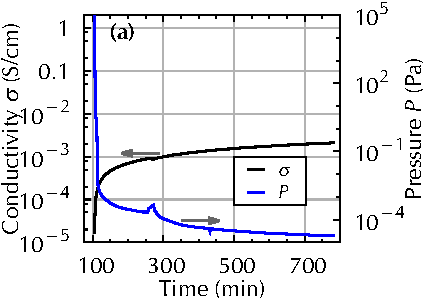
\includegraphics{plot/killing+reanimating-C60-2-evap}%
\hfill
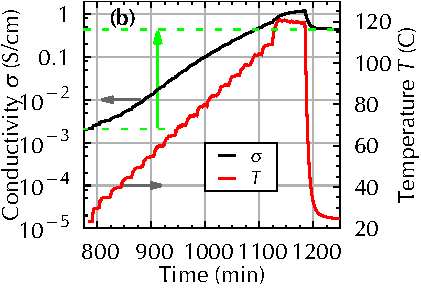
\includegraphics{plot/killing+reanimating-C60-3-heat}%
\setcapwidth[c]{\tmCapWidth}%
\caption
[Conductivity regeneration by vacuum and \insitu heat treatment]
{Conductivity regeneration by (a) vacuum and (b) \insitu heat treatment.}
\label{fig:killing+reanimating-C60-2+2}
\end{figure}
%
After this measurement, the sample is stored again in the vacuum chamber and the pumps are connected and switched on again, evacuating the chamber for several hours. Monitoring the conductivity, an increase up to a value of \c[2.1E-3] is observed at a pressure of \pa{2E-5}, shown in \figref{killing+reanimating-C60-2+2}\,(a).
Hence, 0.1\% of the initial conductivity is restored by the vacuum, indicating that the molecular n-doping is still partly intact.

An additional, much stronger restoring of the conductivity is achieved by slowly heating the sample in vacuum up to \grad{120}, in steps of \K{5} and 20~minutes at each temperature. As shown in \figref{killing+reanimating-C60-2+2}\,(b), W
the conductivity rises significantly with temperature. Cooling the sample back down to \grad{25}, the conductivity stayed at a level of \c[0.44]. Applying several longer cycles of heating to \grad{120} and cooling down to \grad{25} a saturation at \c[0.60] is found.

In conclusion, the initial conductivity of \c[1.88] (\mbox{$100\,\%$}) decreased to \c[1.7E-5] (\mbox{$\approx0.001\,\%$}) after 16~minutes in air. By vacuum treatment \c[2.1E-3] (\mbox{$\approx0.1\,\%$}) and by heat treatment \c[0.60] (\mbox{$\approx32\,\%$}) are restored.

The annealing and removal of oxygen- and hydrogen-related electron traps in pure \CS has already been investigated by the thermally stimulated current (TSC) technique and validated by an enhanced OFET-mobility of four orders of magnitude when thermally annealed after air-exposure\cite{Matsushima2007}. Since for the above discussed sample more than 30\,\% of the initial conductivity is restored by vacuum and heat treatment, it is concluded that the n-doping stays at least partly intact during the air-exposure and is only compensated by oxygen-related traps and p-doping effects.

The same sample is later exposed to air for 3~hours to check for the longtime effects. Again, a drop in conductivity is measured, down to a value of \c[6.6E-7]. Re-evacuating the vacuum chamber leads to \c[2.3E-5] and heat treatment to \c[0.03]. Thus, the much longer air-exposure reduces the final conductivity by an additional factor of 20. The final value is still above the conductivity of a freshly fabricated and thermally annealed sample of \CS doped by \C[0.014] of the air-stable precursor n-dopant \aob that will be presented and discussed in the following chapter. However, it seems evident that the longer exposure degrades more \WPd molecules within the \CS layer.

%
\begin{table}[b]
\centering
\caption
[Effect on air-exposure on \c, \Es and \Eact]
{Overview of the effect on air-exposure on the observables conductivity \c, Seebeck coefficient \S, \EsLong \Es and \EactLong \Eact. All measurements performed on the same sample of \C[0.033] \WPd.}
\label{tab:Pd-Killing}
\begin{tabular}{
c%
c%S[tabnumalign=centre,tabformat=1.2]%
c%S[tabnumalign=centre,tabformat=3.1]%
c%S[tabnumalign=centre,tabformat=3.1]%
c%S[tabnumalign=centre,tabformat=3.1]%
}
\toprule
 & {\c} & {\S} & {|\Es|} & {\Eact}%
\\
measurement after & { \si{\siemens\per\centi\meter}}
 & { \si{\micro\volt\per\kelvin}}
 & { \si{\milli\electronvolt}}
 & { \si{\milli\electronvolt}}
% & { \uVK{}} & { \meV{}} & { \meV{}}
 \\
\midrule %hspace{0.9ex}
 & {($\T[25]$)} & \multicolumn{2}{c}{(\Tm[40])}    & {($\T=25 \text{ to } \grad{70}$)}\\
%
sample preparation
& 2.27
 & & & \\
annealing at \grad{70}
& 2.90
 & $-226.1$
 & \hspace*{1ex}67.7
 & \hspace*{1ex}77.8 \\ 
several loops \grad{25} to \grad{100}
& 1.78
 & $-234.8$
 & \hspace*{1ex}73.5
 & \hspace*{1ex}99.6 \\ 
60\,min at \grad{120}
& 1.88
 &  &     &   \\
16\,min in air
 & \num{1.7E-5}
 &
 &
 &\\
th. annealed in vacuum
 & 0.60 
 & $-262.8$
 & \hspace*{1ex}82.3
 & 103.4 \\ 
180\,min in air
 & \num{6.6E-7}
 &
 &
 & \\
th. annealed in vacuum
 & 0.03
 & $-352.2$
 & 110.3
 & 146.5 \\ 
%
\bottomrule
\end{tabular}
\end{table}
%
%
Besides the conductivity, the \EsLongL and the \EactLongL are measured after vacuum and heat treatment. A summary is given in \tabref{Pd-Killing}. The initial conductivity dropped by a factor of 3 after 16~minutes in air and by an additional factor of 20 after 3~hours in air. 16~minutes in air increased $|\Es|$ by \meV{8.8} to \meV{82.3} ($+12\,\%$) and \Eact by \meV{3.8} to \meV{103.4} ($+4\,\%$). The second exposure of 3~hours in air leads to a gain of $|\Es|$ by another \meV{28.0} ($+34\,\%$) and of \Eact by \meV{43.1} ($+42\,\%$).

The rise in $|\Es|$ corresponds to an increased difference between the \EfLongL and the \EtLongL and hence to a smaller \neLongL. However, after 3~hours of air-exposure the observed $|\Es|$ of the investigated sample of \C[0.033] of \WPd is still lower than the corresponding value of an unexposed sample with a tenth of the \CLong: \mbox{$|\Es|=\meV{167}$} at \C[0.004]. This comparison clearly shows that for the air-exposed sample, at least 10\,\% of the \WPd molecules survive the contact with air and are still providing molecular n-doping. As the measured Seebeck coefficients \S are still negative, compensating p-doping of \CS by oxygen can be excluded.
While the \Es is already strongly affected by 16~minutes of air-exposure, the \Eact only significantly increases after the 3~hours exposure. This suggests a slow but strong change of the charge carrier mobility due to a sustainable formation of electron traps, whereas in case of short exposure most of the induced electron traps can be removed by thermal annealing in vacuum. Furthermore, the larger amount of degradation products that are expected to be present in the layer after 3~hours of air-exposure could act as additional trap states and hence raise \Eact.

Further studies of the degradation mechanism of pure \WPd as well as of layers of \CS doped by \WPd employing the techniques of ultraviolet photoelectron spectroscopy (UPS), X-ray photoelectron spectroscopy (XPS) as well as laser desorption/ionization time of flight mass spectrometry (LDI-TOF-MS) revealed that the majority of the dopant molecules immediately decomposes after air-exposure\cite{TietzeMenke2013}.
However, the remaining \WPd molecules stay intact and slowly degrade with an exponential decay time of \mbox{$\approx13$~minutes}. These findings are attributed to a rise of the IE of \WPd upon charge-transfer, resulting in a protection against oxidation in air.
Consequently, the observed recovery of the conductivity is interpreted as a self-passivation of the molecular n-doping.
Such a passivation mechanism of n-doped layers enables processing steps under ambient conditions, greatly enhancing device fabrication possibilities\cite{Kleemann2012}.

% \pagebreak
\section{Conclusion}\label{sec:ResPdConclusion}
It is found that both dopants, \CrPd and \WPd, are well suited to n-doped \CS. Extremely high conductivities of up to \c[7] are measured, with \CrPd leading to larger values than \WPd. Continuously probing the conductivity for 1~hour after sample preparation, an increase for low and a decrease for high \CLongs is observed. In order to ensure comparable measurement conditions, the samples are thermally annealed prior to the electrical investigations. Afterwards, for both dopants a linear relation of $\c(\C)$ is measured, until at high \C a drop in \c is detected. This reduction is attributed either to a disturbance of the morphology by the large amount of dopants in the layer and hence a drop of the mobility or to a reduced doping efficiency due to clustering of dopants. Seebeck data showed that \S decreases further at high \C and hence the \neLong increases, which suggests that the doping efficiency is not decreasing and the drop in conductivity is due to a reduced mobility. 

Such high conductivities are relevant for device applications, since they enable good charge injection and extraction from the contacts, hence reducing ohmic losses and increasing device performance\cite{Blochwitz1998}.
Furthermore, the substitution of the metal contacts by highly conducting doped organic layers would allow for pure organic devices\cite{Schubert2013}. Additionally, in organic tandem photovoltaic cells, a highly conducting recombination and spacer layer between the two subcells is crucial for device performance\cite{Riede2011,Meiss2011}.

Varying the temperature, the conductivity is found to be in good agreement with a thermally activated hopping transport and an \EactLong \Eact is derived. \Eact decreases with \C for low and moderate \C of both dopants, attributed to a shift of the \EfLong towards the \EtLong. At high \C, the \Eact increases, indicating a disturbance of the morphology of the host material by the large percentage of dopant molecules, in agreement with the conductivity data.

Thermoelectric measurements prove that for all samples electrons are the dominating charge carriers and allow for deriving the energetic difference \Es between \EfLong and \EtLong. This difference is reduced with raising \CLong, as expected from the trend of \Eact. As \Es does not increase at high \C, the observed rise of \Eact and the reduced \c are attributed to changes in the mobility.

AFM studies of the surface roughness yield a rising surface roughness with \CLong in the low and medium doping regime. At high \C, the surfaces are found to be very smooth, which is attributed to a hydrogen film on the surface, attracted by the strongly ionizing dopants and shielding the real topography. Hence, AFM is not a suitable technique to study the morphology of doped layers, as only the surface is probed and material content cannot be resolved.

Air-exposure of n-doped layers is found to lead to fast degradation of the \cLong. However, a large fraction of the initial conductivity can be restored by vacuum and heat treatment. This finding could allow for device processing steps under ambient conditions, greatly enhancing device fabrication possibilities.

Overall it is shown that both dopants are exceptionally well suited for n-doping \CS. Recently, \WPd was successfully deployed in devices \cite{Schunemann2012,Fischer2012}. It would be interesting to study these dopants in hosts of lower \EA to investigate the influence of the molecules' energy levels. First measurements of successfully n-doping ZnPc\footnote{ZnPc is zinc phthalocyanine, $\text{EA}=\eV{3.34}$\cite{Gao2001}} by \WPd\cite{Burtone2013} are promising.


\cleardoublepage
%äöüß
\chapter{Air-Stable n-Dopants in \CS}\label{chap:AirStables}
\addcontentsline{lof}{chapter}{\thechapter\hspace*{1ex} Air-Stable n-Dopants in \CS}

%
\intro{%
In this chapter, the doping mechanisms of two air-stable precursor n-dopants, \aob and \dmbi, are studied and compared to the air-sensitive dopants discussed in the previous chapter. Air-stable n-dopants are much easier to handle and thereby are promising candidates for replacing air-sensitive n-dopants in the future.
In \secref{ResASCond}, the conductivity of differently doped samples is investigated. Directly after sample preparation, a strong gain over time is detected.
Following a thermal annealing step, samples doped by \aob yield a linear, samples of \dmbi a superlinear relation of \cLong to \CLong and possible explanations are discussed.
Temperature-dependent measurements are again indicating a thermally activated hopping process, allowing for deriving an \EactLong.
%
The second \secref{ResAS-S} presents thermoelectric (Seebeck) investigations
for a variation of the temperature and the \CLong. The results are compared to the \EactLong and conclusions for the mobility are drawn.
\Secref{ResASAFM} presents atomic force microscopy (AFM) studies, probing the surface roughness of differently doped samples for indications of clustering or agglomeration of dopants.
The findings are summarized in \secref{ResASConclusion}.
%
Finally, in \secref{ResMeO-DMBI}, \dmbi is compared to a closely related compound, \meodmbiI, and a similar doping mechanism for both is proposed.
}

\newpage%\pagebreak

In the previous chapter, two typical n-dopants with extremely low \IEs are investigated. As such n-dopants are usually unstable in air, handling in an inert atmosphere is required, complicating the fabrication process. In this chapter, the two n-dopants \aob and \dmbi which are air-stable prior to deposition are investigated. Both dopants are salt precursor compounds and form the active dopant compound \insitu during material deposition, as discussed in \secref{Matn}, where the materials' properties are summarized as well.
Again, \CS is used as host material and the same set of experiments is also performed on the air-stable dopants. A selection of the results presented here is published in reference\cite{Menke2012a}.

In general, it is expected that not all deposited air-stable precursor molecules undergo the transformation to the active dopant compounds, hence the doping efficiency of this class of dopants is likely to be lower compared to air-sensitive dopants, where the source material is already the active dopant compound.

Sample preparation and measurements are performed in vacuum, as discussed in sections \ref{sec:ExpSamplePreparation} and \ref{sec:ExpMeasRoutine}.
To ensure optimal preparation conditions for \aob, the chamber is illuminated using a halogen lamp, as proposed by Li\etal\cite{Li2006}. For calculating the \CLong of \dmbiPOH samples, the molar mass of \OHdmbi (\gMole{240.3}) is used, as this material is expected to be formed during deposition, as discussed in \secref{Matn} and later supported by \secref{AS-DMBIs-DopingMech}.

As only small quantities of the rather expensive material \dmbi were available, thinner layers of \nm{20} thickness are produced for samples of high \CLong \Cgr{0.200} instead of the usual \nm{30}. This different layer thickness does not influence the thermoelectric properties and has only little influence on the conductivity via the surface roughness, as discussed in \secref{ExpLayerGroth}.

\section{Conductivity}\label{sec:ResASCond}
The conductivities of layers of \CS doped by various \CLongs of \aob or \dmbi are shown in \figref{MR-Cond-n-AS-evap}. Measurements are performed directly after fabrication of the samples at \T[25].
%
\cBild[t]
{MR-Cond-n-AS-evap}
{As-prepared \cLong \vs \CLong}
{As-prepared \cLongL \vs \CLongL of samples of \CS doped by \aob or \dmbi, measured at \T[25]. Compare to undoped \CS with \mbox{$\c\approx\Scm{2e-8}$}\cite{Li2006}.}
%
As a linear and symmetric current-voltage relation is measured for all samples, and the literature value for the contact resistance between gold and \CS is low\cite{Kitamura2011}, the charge injection can be neglected.
Both materials efficiently dope \CS as the conductivity of the doped layers is several orders of magnitude higher than for undoped \CS, which has been reported to be in the order of \c[2e-8]\cite{Li2006} and which would be below the resolution limit of the Seebeck setup of \c[8.3e-8] as discussed in \secref{ExpResLimit}.
The \cLong can be tuned by doping over two orders of magnitude for each dopant.
At high \C, \dmbi samples reach $\c>\Scm{1}$, whereas for \aob the \c is approximately 100~fold lower at each \C.
Samples doped by \dmbi show a saturation at \Cgr{0.100}, whereas for \aob samples no distinct saturation is visible.
This observation is in contrast to the results determined for high \CLongs of the air-sensitive dopants \CrPd and \WPd (compare \figrefPage{MR-Cond-n-Pd-evap}), as high \C of these materials lead to a decrease in \c.
The result is even more surprising, since higher \CLong of \C[0.650] and \C[0.510] are used for \dmbi and \aob, respectively.
%
This finding suggests that the lighter dopants \aob and \dmbi do not disturb the morphology of \CS as strongly as the heavier and strongly electronegative dopants \CrPd and \WPd. The relation between conductivity and \CLong is discussed in more detail in \secref{ResASCondMR}. First, the change in \cLong directly after sample preparation and the influence of thermal annealing are discussed.

\subsection{Conductivity Changes after Preparation}
As for most sets of materials, prior to further measurements, the conductivity of each sample is continuously probed for 1~hour at a fixed temperature of \T[25]. A strong increase of \cLong with time is detected for both dopants at all \CLongs. In order to quantify the change in \c, the data are fitted according to \eqnrefPage{LongTimeCond-exp}. The resulting fitting parameters are shown in \figref{MR-LongTimeCond-n-AS-fitparameter}.

The fitted maximal relative change $\chi$ is much larger for samples doped by \aob than for \dmbi, with a maximum of $\chi=+350\,\percent$ for \C[0.026] of \aob, compared to $\chi=+76\,\percent$ at a similar \CLong of \C[0.027] of \dmbi. The change $\chi$ detected for both materials is stronger than for \CrPd and \WPd. Furthermore, whereas for \CrPd and \WPd a decrease of \c at $C>\mr{0.040}$ is found, all samples doped by the two air-stable dopants show an increase of \c during the first hour after deposition.

As it has been reported\cite{Li2006} that illumination during deposition can accelerate/enhance the doping process for \aob, it is possible that in this case during sample fabrication the illumination intensity was too low, or that \aob generally needs more time to deploy its full doping capability and therefore shows a much stronger change after preparation than \dmbi. The positive change observed for all \CLongs of both materials might be due to a molecular rearrangement, as the dopants are much smaller than \CS and might be able to diffuse until they find a suitable host molecule to donate their electron to.

The time constant $\tau$ is smaller for almost all \dmbi samples than for the \aob samples, corresponding to a faster approach of saturation. While the values of the \dmbi samples scatter around $\tau=0.6\pm0.3$~hours, for \aob $\tau$ drops with rising \CLong from 1.7~hours at \C[0.007] to 0.2~hours at \C[0.510]. The reason for this difference is not clear at present.

\cBild
{MR-LongTimeCond-n-AS-fitparameter}
{Conductivity change during first hour after preparation, fitting parameters}
{Fitting parameters of conductivity change during the first hour after sample preparation, according to \eqnrefPage{LongTimeCond-exp}: (a) maximal relative change $\chi$ reached after $t\gg\tau$ (b) time constant $\tau$ describing the speed of the change.
}

\subsection{Relation of Conductivity to Doping Concentration} \label{sec:ResASCondMR}

As discussed in \secref{ResPdCondMR}, all samples are thermally annealed prior to further measurements, in order to ensure stable measurement conditions. They are slowly heated from \T[25] to \grad{100} and kept at this temperature for 60~minutes. Afterwards, the samples are slowly cooled down and the measurement routine (compare \secref{ExpMeasRoutine}) is started with a conductivity measurement at \T[25], where no further change of \c over time is detected.

\cBild
{MR-Cond-n-AS-evapVS25}
{Conductivity before and after thermal annealing}
{Conductivity before (filled symbols) and after (empty symbols) thermal annealing (at \T[100]) for \CS doped by (a) \aob and (b) \dmbi. The dashed lines represent a slope of 1.0 for \aob and a slope of 2.0 for \dmbi.
}

In \figref{MR-Cond-n-AS-evapVS25}, the conductivity after thermal annealing is compared to the conductivity measured directly after sample preparation (compare \figref{MR-Cond-n-AS-evap}), both measured at \T[25]. After annealing, a strong increase by two to three orders of magnitude is observed for the \aob samples, demonstrating that illumination alone is not sufficient to deploy the full doping capability of \aob. The conductivity of the \dmbi samples increases to a lesser extent, by a factor of about 10.
Thermal annealing seems to accelerate the effect responsible for the change of conductivity during the first hour after sample preparation. This observation is consistent with the results for the air-sensitive dopants \CrPd and \WPd, compare \secref{ResPdCondMR}.

For the air-sensitive dopants, three different contributions to the change of conductivity are discussed in the previous chapter: Firstly, residual quantities of O\sub{2} and moisture, present in the vacuum chamber, could react with the n-doped layers and reduce the conductivity. Thermal annealing might remove these impurities and hence increase the conductivity. Secondly, small rearrangements of the molecules could lead to an increase in conductivity. Thirdly, a phase separation and demixing of host and dopant at high \CLong may reduce the conductivity due to shielding of dopants.
As the observed changes of the conductivity are all positive and much stronger than for the air-sensitive dopants, the changes are most likely due to a major additional contribution. Most probably, the transformation which forms the active dopant compounds from the air-stable precursor molecules is not completed by all molecules during sample deposition. Instead, the process continues afterwards and can be accelerated by heating the doped layer.

After the thermal annealing step, an increasing conductivity with \CLong is measured for both dopants.
For \aob, a linear correlation between \CLong and conductivity, highlighted by the dashed line of slope 1.0 in \figref{MR-Cond-n-AS-evapVS25}\,(a), is found for over two orders of magnitude with no saturation visible in the data. Thus, each additional dopant molecule contributes identically to the increase of \c.
At the highest \C[0.510] of \aob, \c[0.6] is measured at \T[25]. This value is higher than the previously reported data\cite{Li2006}, which is due to the higher \CLong and optimized preparation conditions, \eg illumination during evaporation and the thermal annealing step.

The conductivity of almost all \dmbi samples is one order of magnitude higher than for \aob at corresponding \CLongs, when measured at \T[25] after the thermal annealing.
A highest value of \c[5.3] is found at \C[0.650], which is even \Scm{1} higher than the record conductivity for the air-sensitive dopants (after thermal annealing), summarized in \figref{MR-Cond-n-PdvsAS}.
The \dmbi samples show a different tendency than the samples doped by \aob, as for low \C the \c increases superlinearly with \C at a slope of 2.0, highlighted by the dashed line in \figref{MR-Cond-n-AS-evapVS25}\,(b). At \Cgr{0.150} the slope is reduced, first to a value in the range of 1.0 and later a saturation is detected.
The reduced slope for \Cgr{0.150} of \dmbi, might be attributed to aggregation of dopant molecules, leading to a decreasing doping efficiency\cite{Mityashin2012a}, or to a disturbance of the morphology resulting in a lower mobility\cite{Kleemann2012a}. In \secref{ResASAFM}, AFM studies on doped layers are presented, showing peaks arising from the layer for \Cgr{0.150}, which makes both explanations plausible.

\cBild
{MR-Cond-n-PdvsAS}
{Comparing the conductivity of \CS doped by air-stable and air-sensitive dopants}
{Comparing the conductivity after thermal annealing of samples of \CS doped by air-stable (\aob and \dmbi, \T[25]) and air-sensitive (\CrPd and \WPd, \T[30]) dopants. The dashed lines of slopes 1.0 and 2.0 are guides to the eye.}

In agreement with \aob, samples doped by the air-sensitive dopants \CrPd and \WPd show a linear relation of \c to \C as summarized in \figref{MR-Cond-n-PdvsAS}.
The superlinear increase for \dmbi suggests that there may be a difference in the doping or transport mechanism when \CS is doped by \dmbi. A conductivity slope of more than 1.0 has been reported as well as predicted by various groups and models, as discussed below.

Our collaborators from Stanford University observed a similar slope in the range of 2.0 for \PCBM\footnote{\PCBM is \PCBMLong} doped by the neutral dopant \Ndmbi\footnote {\Ndmbi is \NdmbiLong} which is closely related to \dmbi\cite{Wei2010}.
Gregg\etal\cite{Gregg2004Review} expected a superlinear relation for all excitonic semiconductors, due to a decrease of exciton binding energy with increasing \CLong.
Männig\etal\cite{Maennig2001} interpreted a superlinear increase of the conductivity upon doping as indication for shallow states in combination with percolative transport and a sublinear increase as indication for deep donors states.
%
Both of these models can be used to explain the mechanism of doping of \CS with \dmbi but they are at odds with the observations for the other three n-dopants (\aob, \CrPd and \WPd). However, the fact that the conductivity increase is not superlinear for the other dopants does not invalidate these models.

According to Arkhipov\etal\cite{Arkhipov2005}, doping generates deep Coulombic traps in disordered organic semiconductors, which can reduce the mobility with increasing \CLong. These traps may be generated by changes of the energy levels due to the presence of ionized dopants or could be created by disturbances in the morphology. \OHdmbi, being the active dopant compound formed from \dmbi is the smallest of the investigated n-dopants (with a diameter of \nm{\approx1.0}, compare \figrefPage{mat}), thus it may cause small morphological disturbances of the \CS host molecules, leading to a superlinear increase of \c at \Ckl{0.100}. To validate this hypothesis, morphological analysis of the molecular arrangement by techniques like X-ray diffraction or refraction should be performed.
%
Since \aob is the least efficient dopant (with respect to the conductivity), it might have a deeper donor state compared to \dmbi resulting in generation of trap states and hence a decreasing mobility with rising \CLong. The presence of traps could be investigated \eg by methods like impedance spectroscopy (IS)\cite{Burtone2012} or thermally stimulated current (TSC)-based methods like charge-based deep level transient spectroscopy (Q-DLTS)\cite{Gaudin2001}. This however is beyond the scope of this thesis.

A deep donor state for \aob agrees with the results of Harada\etal\cite{Harada2007} who demonstrated that the OFET-mobility of \aob-doped \CS decreases upon doping. Increasing \C from \mr{0.010} to \mr{0.075}, the mobility dropped by a factor of three, which corresponds to a slope of $-0.5$ in a logarithmic scale. The decreasing mobility was attributed to a scattering of charge carriers at ionized impurities, introduced by doping.
Even if the \neLongL increased superlinearly with \C for \aob samples as well, a decreasing mobility would lead to a reduced slope of $\c(\C)$.

Olthof\etal\cite{Olthof2012} have reported for the material system of \CS doped by [RuCp$^*$(mes)]$_2$%
\footnote{[RuCp$^*$(mes)]$_2$ is ruthenium(pentamethylcyclopentadienyl)(1,3,5,-trimethylbenzene)}
that at \Ckl{0.001}, a superlinear slope of $\c(\C)$ is attributed to filling of trap states. As the \CLongs investigated in this thesis are above \mr{0.001}, filling of host material trap states is not likely to be responsible for the superlinear slope.
Olthof\etal furthermore reported on a gain in mobility upon doping, which they again attributed to filling of trap states. As they have assumed a concentration-independent doping efficiency of \DopEff[100] to calculate the \neLongL from \C, their approach is contrary to the model of a threshold doping concentration presented by Mityashin\etal\cite{Mityashin2012a}, as discussed in \secref{Theo-org-Doping-Mechanisms}. Up to now, it is not clear which model is correct for the material system presented here.

Another considerable reason leading to a superlinear increase of conductivity for \dmbi compared to \aob would be that as in these systems charge carriers are transported along a manifold of states distributed in energy and space, a charge carrier density-dependent mobility is expected. Upon increasing the charge carrier density, the mobility may increase if the low-lying localized states are filled, leading to a transport dominantly along the denser part of the density of states. This phenomenon is observed in OFETs where these states are filled by the gate bias. It is possible that for efficient doping a similar effect may be present. In such a case the conductivity increases superlinearly with \C. However, dopants such as \CrPd and \WPd, which lead in \CS to conductivities similar to \dmbi, as summarized in \figref{MR-Cond-n-PdvsAS}, do not show such a behavior, suggesting that this phenomenon may not be dominant in this system.

% \FloatBarrier
\subsection{Temperature Dependence of the Conductivity}
In analogy to the samples of \CS doped by the air-sensitive dopants in the previous chapters, the conductivity after thermal annealing is probed at different temperatures between \T[25] and \grad{100} and is found to rise with temperature. \Figref{T-Cond-n-AS} displays the measured data of all samples in Arrhenius plots. A linear relation is found, in agreement with the results for the air-sensitive dopants and the literature, indicating a thermally activated transport mechanism for which again an \EactLongL can be derived employing \eqnrefPage{CondActivation}.

\cBild[b]
{T-Cond-n-AS}
{Temperature dependence of the conductivity}%
{Temperature dependence of the conductivity of \CS doped by (a) \aob and (b) \dmbi. Lines are fits using \eqnrefPage{CondActivation}.}

The resulting values of the differently doped samples range from \Eact[63] for low to \meV{241} for high \CLongs and are illustrated in \figref{MR-Eact-n-AS}. They are well below the previously reported value for undoped \CS of around \meV{640}\cite{Li2006}.
The \Eact is higher for the \aob samples than for the \dmbi ones, excluding the lowest doped \dmbi sample.
While for the \aob samples \Eact slowly drops with rising \CLong, the \dmbi samples yield a much stronger decrease and a saturation at \mbox{$\Eact\approx\meV{75}$} at \Cgr{0.150}. At the same \CLong, a reduction of the superlinear slope of $\c(\C)$ is observed in \figrefPage{MR-Cond-n-AS-evapVS25}.

\cBild[t]
{MR-Eact-n-AS}%
{Activation energy of the conductivity}%
{Activation energy of the conductivity \Eact, derived from the temperature dependence of the conductivity $\c(T)$ in the range of \T[25] to \grad{100} shown in \figref{T-Cond-n-AS}, using \eqnrefPage{CondActivation}.
}%

As discussed in \secref{ResPdCondEact}, the drop of \Eact with increasing \CLong is attributed to a shift of the \EfLong \Ef towards the \EtLong \Et of \CS. This shift leads to a reduction of the temperature dependence of the density of free electrons $\ne(T)$.

%
At high \CLongs of \aob, a rapid drop of \Eact is observed. This may be attributed to the fact that at high \C, \aob (which is not as efficient as \dmbi) is able to fill up the deeper states of the density of states and to contribute more to the shift of the \Ef. Such a process is similar to what is known as compensation in classic semiconductor theory. When compensation is the dominant effect, \Ef is pinned to the dopant level. If compensation is no longer the main effect, \Ef shifts towards the conduction band minimum \Ec (for n-doping).
A higher dopant level of \dmbi would lead to a more efficient filling of the energetically lower lying low-mobility states of the hosts density of states, thus generating an overall higher mobility along with a lower \Eact.

In case of \CS n-doped by the air-sensitive dopants \CrPd and \WPd, at high \CLongs an increase of \Eact along with a decrease of \c is found. This behavior is not observed for the lighter dopants \aob and \dmbi, even though the \CLongs are higher. Since this effect is attributed to a disturbance of the morphology of the host material by the large percentage of dopant molecules, \aob and \dmbi are understood to lead to less disturbance, which might be attributed to their smaller size. AFM investigations, presented in \secref{ResASAFM}, show that with rising \CLong more and more artifacts are arising on the samples' surfaces for \CS doped by each of the two air-stable dopants. These artifacts are an indication for agglomeration of dopants or charge-transfer complexes.

% \newpage
\section{Thermoelectric Measurements}\label{sec:ResAS-S}
\subsection{Temperature Dependence of the Seebeck Coefficient}
\label{sec:ResAS-S-T}
%
%
Along with the conductivity investigations, thermoelectric (Seebeck) studies are performed. The probed Seebeck coefficients \S for layers of \CS doped by \aob or \dmbi are presented in \figref{T-S-n-AS}\,(a) and (c). As expected, they are negative in sign, thus, for all samples, electrons are the dominating charge carrier species and hole conduction along the dopant molecules is not observed. The resulting values range from \S[-120] to \uVK{-580} and a decrease of $|\S|$ with increasing \C is detected, similar to the results for the air-sensitive dopants in \secref{ResPd-S}.

\cBild[b]
{T-S-n-AS}%
{Temperature dependence of the Seebeck coefficient}%
{Temperature dependence of the Seebeck coefficient \S for \CS doped by \aob and \dmbi in (a) and (c). At the right side, in (b) and (d), the relative changes of \S are illustrated, normalized to the \Tm[40] measurements.
}

In order to investigate the influence of the mean temperature \Tm, the relative changes of \S, normalized to the measurements at \Tm[40], are depicted in \figref{T-S-n-AS}\,(b) and (d). A temperature of \grad{40} is chosen, as it is a device-relevant temperature and allows for more stable temperature control than \Tm[30]. In the investigated range of \Tm[30] to \grad{100} all \dmbi samples except the two lowest doped ones show a strong gain of $|\S|$ with \T, in the order of $+10\,\%$ to $+25\,\%$ (compare \figref{T-S-n-AS}\,(d)). There is no clear relation between \CLong and the magnitude of increase present in the data.
In case of doping by \aob, even stronger increases by up to $+45\,\%$ are recorded, but on the other hand four of the nine samples yield a more or less temperature-independent \S. Thus, there is again no clear trend visible.

As the temperature dependence of \S for samples doped by the air-sensitive dopants \CrPd and \WPd, discussed in \secref{ResPd-S-T}, is measured in a smaller temperature range of \Tm[30] to \grad{70}, the 4 dopants can only be compared in this range, where the relative changes are similar.
It is not clear up to now why for \aob and \dmbi the strongest change is recorded at high \CLongs, whereas for \CrPd and \WPd the weakly doped samples show the strongest change.

\subsection{Relation of Seebeck Coefficient to Doping Concentration}
%
\cBild[b]
{MR-See+Es-n-AS}%
{Seebeck coefficient and derived \EsLong}
{Seebeck coefficient \S and derived \EsLongL at \Tm[40].}
%
Comparing the Seebeck coefficients at \Tm[40] for different \CLongs, a reduction of $|\S|$ with rising \C is found for both dopants, ranging from \S[-714] to \uVK{-124}, as illustrated in \figref{MR-See+Es-n-AS}.
Using \eqnrefPage{S-Es-org}, again the energetic difference \Es between the \EfLong \Ef and the \EtLong \Et can be derived:
\begin{align}
 \Es =\S \cdot e \cdot \T \quad \text{ with } \quad\Es := \Ef - \Et
\PUNKT
\tag{\ref{eq:S-Es-org}}
\end{align}
This quantity is drawn as the right hand axis in \figref{MR-See+Es-n-AS}.
A maximum of \Es[-183] is measured for the lowest \CLong of \C[0.0067] of \aob. Analogously, for \dmbi the largest \Es[-147] is measured for the lowest \CLong of \C[0.013].

Following the trend of \S, the value of \Es drops with rising \C for both dopants, which corresponds to a shift of the \EfLong \Ef towards the \EtLong \Et and thus an increasing charge carrier density \ne, which is in agreement with the observations of the air-sensitive dopants.
%
At high \CLongs, a value of $\Es<\meV{65}$ is derived for both dopants. This saturation value is somewhat higher than observed for the air-sensitive dopants, where $\Es<\meV{50}$ was found in \secref{ResPd-S-MR}. Again, the saturation can be explained by a pinning of \Ef close to \Et via degenerate doping.

\subsection{Comparison of Seebeck Energy and Activation Energy}
\label{sec:ResAS-EsEact}

%
\cBild[b]
{MR-Es+Eact-AS}
{Comparison of \Es and \Eact}
{Comparison of \EsLongL and \EactLongL. \Es is measured at \Tm[40], \Eact is fitted from the conductivity data presented in \figref{T-Cond-n-AS} in the range of \T[25] to \grad{100}.}

In \figref{MR-Es+Eact-AS}, the \EsLongL is compared to the previously discussed \EactLongL, for \aob and \dmbi in part (a) and (b), respectively.
The \dmbi samples show for almost all \CLongs a reasonable agreement of the two energies, whereas for all \aob samples a difference of \mbox{$\Eact\approx\Es+\meV{50}$} is observed.

If the temperature dependence is Arrhenius-like, the difference between \Eact and \Es for the \aob samples is attributed to an activation of the mobility, as discussed in \secref{ResPd-EsEact}.
For the air-sensitive dopants, a discrepancy between \Eact and \Es is observed only at high \C, which is attributed to a disturbance of the morphology by the large number of dopant molecules.
Such a temperature-activated mobility is another indication that \aob introduces deep lying trap states.
%
However, the temperature dependence of the mobility may differ from a simple activated case%
, as discussed in \secref{ResPd-EsEact}.

Harada\etal\cite{Harada2007} have reported a temperature-independent OFET-mobility for \CS doped by \C[0.010] to \mr{0.075} of \aob in the range of \T[30] to \grad{100}. The reason for the difference in results might be the filling of the trap states by electrons accumulated within the OFET channel region by applying a gate-source potential. However, as discussed in \secref{ResPd-EsEact}, the high applied fields required for OFET experiments are expected to affect the occupation of the density of states and thus the resulting mobility.

\section{Morphology}\label{sec:ResASAFM}
%
\cBildDraw[p]{afm-AS-images}%
{AFM images}%
{AFM images of a selection of Seebeck samples. \mbox{(a-c)}: \CS doped by \aob, \mbox{(d-f)}: \CS doped by \dmbi. Note the different height scales. Parameters: $\um{5}\times\um{5}$ scan area, \nm{30} layer thickness for \aob samples and \nm{20} for \dmbi, measurements performed in air after electrical investigations and thermal annealing.
}

\cBild[p]
{MR-AFM-AS}%
{AFM root-mean-square surface roughness \rms}
{AFM root-mean-square surface roughness \rms of all studied samples, scanned on an area of $\um{5}\times\um{5}$, as depicted in \figref{afm-AS-images}.
}

Atomic force microscopy (AFM) investigations are performed on the same samples electrically investigated and discussed above to check for an influence of the presence of dopant molecules on the morphology of the layers.
As AFM studies could only be performed in air, after the electrical investigations the samples are removed from the vacuum chamber and the Seebeck setup and stored in air for several hours before and during the AFM measurement.
Therefore, the results might differ from freshly prepared samples, investigated in an inert atmosphere.
The topographies of selected samples are depicted in \figref{afm-AS-images}, each scanned on an area of $\um{5}\times\um{5}$.
As a figure of merit, the root-mean-square surface roughness \rms is written onto the images and summarized against the \CLong in \figref{MR-AFM-AS}.
%
The different layer thicknesses of the samples (mostly \nm{20} for \dmbi and \nm{30} for \aob samples, as discussed earlier), make the absolute numbers of the \rms not directly comparable, but the trends are reliable.
Due to a larger scan area of $\um{5}\times\um{5}$, compared to $\um{2}\times\um{2}$ used for the measurements on the air-sensitive dopants, the \rms values are not directly comparable to these values either.

At low to medium \CLongs, a smooth surface is detected for both dopants, in agreement with the findings for the air-sensitive dopants. With rising \CLong the roughness increases for both dopants and artifacts become visible on the surface. A similar trend is observed for both dopants: At \C[0.240] many small spikes are present, whereas at higher \CLongs fewer but much larger spikes are found, which lead to a saturation of the \rms value. The largest artifacts are observed for the \dmbi samples with peaks of up to \nm{75} reaching out of a layer with a nominal thickness of \nm{20}.
These artifacts are an indication for agglomeration of dopants or charge-transfer complexes.
Compared to the air-sensitive dopants, the increase of the roughness occurs at higher \CLongs, which can be explained by the smaller weight and size of the air-stable compounds. The rough surfaces found for \Cgr{0.100} suggest that for devices where smooth layers are required in order to prevent shortcuts, lower \CLongs should be used.
It is not clear if the surface structures are generated by the thermal annealing step, as only annealed samples are investigated.

Contrary to these results, the investigations of the air-sensitive dopants yield smooth surfaces at high \CLongs, which is interpreted as a measurement artifact due to the presence of a hydrogen film on the surface, attracted by the ionized dopants. As the topography is visible here, it is suggested that these dopants do not react as strongly with the ambient.
%
\nopagebreak[0] % ensure that no new page in started
\section{Conclusion for \aob and \dmbi}\label{sec:ResASConclusion}
Despite the expectation of a lower doping efficiency for the air-stable dopants compared to the air-sensitive dopants, due to the required transformation to form the active dopant compounds from the air-stable precursor, doping \CS by \dmbi leads to comparable results to \CrPd and \WPd, whereas \aob yields lower values. Even the values achieved using \aob should be sufficient for device application in photovoltaic cells, as \CS has a high charge carrier mobility.
All doped \CS layers are stable up to \T[100], being above the evaporation temperature of the \aob precursor compound. A strong increase of conductivity over time is observed for \aob samples directly after sample processing, suggesting that the doping process is not completed during the deposition. Thermal annealing greatly enhances the conductivity of \aob samples and is required to ensure stable measurement conditions. A less pronounced effect is observed for \dmbi, yielding already high conductivities directly after sample fabrication. After annealing, \dmbi generates one order of magnitude higher conductivities in doped layers, with a maximum of \c[5.3], comparable to the values for the air-sensitive dopants \CrPd and \WPd.

While for \aob layers, as well as for the air-sensitive compounds, a linear relation of $\c(\C)$, a superlinear relation is found for \dmbi.
This could either be due to a difference in the doping mechanism or to a difference in the transport properties of the doped system.

With increasing \CLong, the \EactLong for both dopants drops significantly. The Seebeck studies show the same tendency for the energetic difference between the \EfLong and the \EtLong. For \aob, the magnitude of this difference is smaller than the \EactLong. It is concluded that the mobility in the \aob layers is thermally activated and that the IE of \aob is expected to be larger than the IE of \OHdmbi, being the proposed active dopant formed from \dmbi.

AFM surface scans yield a strong gain in surface roughness for \Cgr{0.100} of both dopants. This suggests that for devices, where smooth layers are required in order to prevent shortcuts, lower \CLongs should be used.

Overall, the dopant \dmbi yields a better doping efficiency compared to \aob. The achieved conductivities are comparable to the results obtained for the air-sensitive dopants \CrPd and \WPd, making \dmbi a promising candidate for application in future devices, especially as \dmbi is air-stable prior to processing.

In the next section, \dmbi is compared to a closely related novel dopant, namely \meodmbiI.

\newpage
\section{\texorpdfstring{\meodmbiI}{o-MeO-DMBI-I}}
\label{sec:ResMeO-DMBI}
Based on the experience with the commercially available n-dopant compounds \Ndmbi and \dmbi, our cooperation partners Peng Wei and Benjamin D. Naab from Professor Zhenan Bao's group of Stanford University started designing and synthesizing new dopants. One promising material they developed is \meodmbiI. Its structure is similar to \dmbi, as illustrated in \figref{mat}\,(b) on page~\pageref{fig:mat} and its key parameters are presented in \secref{Matn}. This material is stable during vacuum deposition, and first experiments performed in Stanford indicated excellent doping performance comparable to \dmbi. Consequently, further investigations were started in Dresden.
A selection of the results presented here is published in reference\cite{Wei2012}.

Obvious differences compared to \dmbi are that \meodmbiI is a white crystalline powder, whereas \dmbi is a yellow fuzzy structured material. The deposition temperature of \meodmbiI is found to be around \Tdep[185], being \K{75} higher than for \dmbi (compare \tabref{MatProp}). This allows more stable temperature control during layer deposition. The similarity of the chemical structures of both compounds suggests a similar doping mechanism.

\subsection{Doping Mechanism}\label{sec:AS-DMBIs-DopingMech}
A sudden increase of base pressure in the vacuum chamber by more than one order of magnitude is detected as soon as the deposition of \meodmbiI starts. At \T[100] the base pressure is \pa{7.3e-6} with no detectable deposition rate, whereas at \T[185] during layer deposition a pressure of \pa{1.6e-4} is observed. The pressure remains at this level until the temperature is decreased to a level where the deposition stopped. In order to investigate these observations, a mass spectrometer (Pfeiffer QMG220) is installed at the vacuum chamber.

%
\cBild[t]
{massSpekDMBI}
{Mass spectrum during \meodmbiI deposition}
{Mass spectrum obtained during \meodmbiI deposition at a material temperature of around \grad{185} at $\druck=\pa{1.6e-4}$, probed at a scan speed of \SI{2}{\second\per\atomicmass}. Left inset: zoomed region of main structure. Right inset: high resolution measurement at \SI{20}{\second\per\atomicmass}.}
%
%
In \figref{massSpekDMBI}, a wide mass spectrum scan from \u{0} to \u{300} performed at a rate of \SI{2}{\second\per\atomicmass} is presented, which is probed at a dopant source temperature of \grad{185}.
Two dominant peaks around \u{127} and \u{142} are present, each having several side peaks. The relative heights of the peaks are found to vary between different measurements, probably related to changes in pressure during the long scan time.
The left inset of \figref{massSpekDMBI} is a zoom into the area of these two main peaks, displaying the substructure.
The peak at \u{127} is assigned to ionized iodine I$^-$ (\u{126.9}), the smaller one next to it to HI (\u{127.9}). Iodine has a boiling point of \grad{184.3} at atmospheric pressure, hence the freed iodine is expected to turn into the gas phase at \grad{185} in vacuum. The second large peak around \u{142} is attributed to CH$_3$I (\u{141.9}). These findings suggest that the material \meodmbiI loses its iodine atom upon deposition, forming \meodmbi as active dopant compound.

A high resolution mass spectrum obtained at a $10\times$ slower scan speed of \SI{20}{\second\per\atomicmass}, presented as right inset of \figref{massSpekDMBI}, resolved a peak at \u{254.3} that nicely fits to the expected dopant compound \meodmbi and is above the value expected for I$_2$ at \u{253.8}.
As no mass peak for a neutral radical at \u{253.3} is observed, it is hypothesized that the doping mechanism is the following: \meodmbiI is reduced during evaporation under high vacuum to form \meodmbi (compare \figref{mat}\,(e1) on page~\pageref{fig:mat}), which then transfers an electron to a \CS molecule.
Therefore, in order to calculate the \CLong of samples doped by \meodmbiI, the molar mass of \meodmbi ($\MM=\gMole{254.3}$) has to be used.

Further investigations on the doping mechanism were performed by our partners at Stanford University. X-ray photoelectron spectroscopy (XPS) measurements on pure \meodmbiI layers fabricated by vacuum deposition yielded no iodide peak, indicating that \meodmbiI is reduced and lost I$^-$ during the evaporation. Furthermore, this suggests that the lost I$^-$ does not contaminate the deposited layers.\cite{Wei2012}

Due to the structural similarity of \meodmbiI and \dmbi (compare \figref{mat}\,(b) on page~\pageref{fig:mat}) it is expected that \dmbi undergoes a similar transition to form the active dopant compound \OHdmbi during deposition of the material. The proposed reaction is illustrated in \figref{mat}\,(e2).
Thus, in order to calculate the \CLong of samples doped by \dmbi, the molar mass of \OHdmbi ($\MM=\gMole{240.3}$) has to be used.

\subsection{Comparison to \dmbi}%\texorpdfstring{\dmbi}{DMBI-POH}

\cBild[b]
{MR-Cond-n-DMBIs}
{\meodmbiI \vs \dmbi: conductivity}
{Conductivity of \CS doped by \meodmbiI and \dmbi, before (filled symbols) and after (empty symbols) thermal annealing (at \T[100]), measured at \T[25]. Note the two samples of identical \C[0.246] of \meodmbiI proving the reproducibility. The dashed line represents a slope of 2.0.}

\Figref{MR-Cond-n-DMBIs} compares the conductivities of \CS layers doped by \meodmbiI to the data for \dmbi, presented in \secref{ResASCondMR}.
For the new compound \meodmbiI, the conductivity after thermal annealing (empty symbols) is in the same range as for the \dmbi samples. The lowest doped sample of \C[0.027] of \meodmbiI has an almost identical value of \c[0.174] to the corresponding sample of \dmbi with \c[0.162] at \C[0.027]. A maximum of \c[10.9] is measured for \C[0.310], being more than twice as high as the record value observed for \dmbi as well as for \CrPd and \WPd. At even higher \CLongs of \meodmbiI, the \cLong decreases, in contrast to \dmbi, where a saturation is observed.
The relation of the conductivity to the \CLong follows the same trend for both materials. Samples doped by \meodmbiI show as well a superlinear increase of $\c(\C)$, as the dashed line in \figref{MR-Cond-n-DMBIs}, possessing a slope of 2.0, indicates. Reproducibility is proven by two samples of \C[0.246] of \meodmbiI showing almost identical values.

The most interesting difference between the two dopants is that for the new compound, the thermal annealing after preparation has only little effect on the conductivity. While for most \dmbi samples a gain on almost one order of magnitude is found, the strongest change observed for the \meodmbiI samples is an increase by a factor of 3.6, found for the lowest doped sample. Hence, for \meodmbiI thermal annealing is not necessary to achieve high conductivities.

Surprisingly, reproducing the samples in our group's multi chamber vacuum tool was not successful. The conductivities of 5 samples with \CLongs from \C[0.150] up to \mr{0.700} were between \Scm{0.03} and \Scm{0.3} with no clear relation between \c and \C. Thermal annealing made it possible to reach comparable conductivities to the samples fabricated in the Seebeck setup. The main differences between the chambers is that in the multi chamber tool, the base pressure is one order of magnitude lower, in the range of \pa{8E-7}. During deposition a pressure in the range of \pa{2E-6} is measured, being almost a factor of 100 lower than the increased pressure recorded during fabrication in the Seebeck setup.
Hence, most probably the Seebeck chamber with the worse base pressure has more leakage gas flow through the chamber towards the pumps. It might be possible that this material flow transports the iodine gas (produced by formation of \meodmbi from \meodmbiI) away from the deposited layer, whereas in the multi chamber tool iodine might reach the substrate, leading to a reformation of \meodmbiI.
Another difference of the multi chamber tool compared to the Seebeck setup is a different pressure sensor that generates an electric arc, illuminating the chamber and maybe affecting the materials during deposition. However, deactivating the sensor had no affect on the samples.

\cBild[t]
{MR-Es+Eact-DMBIs}
{\meodmbiI \vs \dmbi: comparing \Es and \Eact}
{Comparing \EsLongL (empty symbols) and \EactLongL (filled symbols) of \CS doped by \meodmbiI and \dmbi. \Es is measured at \Tm[40], \Eact is derived from the range of \T[25] to \grad{100}.}

Temperature-dependent conductivity and Seebeck measurements are performed on the \meodmbiI samples as well. A comparison to \dmbi is shown in \figref{MR-Es+Eact-DMBIs}. Seebeck measurements (empty symbols) of the two compounds are in reasonable agreement, leading to the assumption that the doping efficiency of \meodmbiI is comparable to \dmbi. The \EactLong \Eact (filled symbols) is somewhat lower for most \meodmbiI samples and closer to \Es, indicating a smaller contribution of the mobility to \Eact.

In conclusion, there are several indications for \meodmbiI and \dmbi having a similar doping mechanism. Comparable values of \c, \Es and \Eact, as well as a superlinear increase of $\c(\C)$ are observed. The high maximum of \c[10.9] for \meodmbiI is the record value measured for all material combinations during this thesis. Its deposition temperature in the range of \Tdep[185] makes the rate better controllable than for \dmbi, which is deposited as \Tdep[110]. Furthermore,  for this compound thermal annealing is not necessary to achieve high conductivities, at least not in the Seebeck setup. Hence, \meodmbiI is a promising new dopant that should be tested in devices.


\cleardoublepage
% äöüß
\chapter{p-Dopants in Amorphous Hosts}\label{chap:P-Doping}
\addcontentsline{lof}{chapter}{\thechapter\hspace*{1ex} p-Dopants in Amorphous Hosts}

\intro{%
After investigating n-doping in the last two chapters, this chapter investigates p-doped material systems. Two hosts and two dopants are chosen in order to study the influence of the molecular energy levels.
While the host material used for the n-doping experiments is the exceptionally well conducting polycrystalline \CS, the two hosts studied in this chapter are more typical amorphous \OSCs with approximately five orders of magnitude lower mobilities.
In \secref{ResP-Cond}, the conductivity of differently doped samples is studied. Afterwards, it is investigated how the \cLong is influenced by the temperature, which again supports a thermally activated hopping process and therefore allows to derive an \EactLong.
\Secref{ResP-S} presents thermoelectric (Seebeck) investigations for a variation of the temperature and the \CLong. The results are compared to the \EactLong and conclusions for the mobility are drawn. In \secref{ResP-Degradation}, the thermal stability is investigated and finally, in \secref{ResP-Conclusion}, the results are summarized.
}

\pagebreak

One major difference of p-doping to n-doping is that p-doped layers are usually degrading more slowly under air-exposure or under contact with residual quantities of O$_2$ present in the vacuum chamber. The reason is that oxygen leads to a p-doping as well\cite{Hamed1993} and hence to traps in n-doped layers.

Four different material combinations are investigated in this chapter. As host materials, \meo and \lili are chosen which have been both used in OLEDs\cite{Reineke2009} and OPV\cite{Maennig2004,HermenauRiedeLeo2012}. The host materials are selected to have slightly different \IEs, in particular \mbox{$\text{IE}=\eV{5.07}$} for \meo\cite{Tietze2012} and \eV{5.23} for \lili\cite{Meerheim2011}.
Two different p-dopants, \FS and \CSF, are studied, having estimated electron affinities of \mbox{$\text{EA}\approx\eV{5.00}$} for \FS\cite{Tietze2012,WellmannDiss} and \eV{5.38(30)} for \CSF\cite{Meerheim2011}. Since different techniques for the estimations have been used and the errors are rather large, the true values may differ.
From the measured values of the hosts' IEs and the estimated values of the dopants' EAs, the doping is expected to be more efficient for \CSF, whereas for \FS very low doping efficiency is expected.
However, energy levels are merely a rough guide to predict the doping effectiveness, as microscopic details like spatial arrangements of orbitals play an important role as well. While the two hosts are of similar weight, the dopant \CSF is almost 4~times as heavy as \FS.
Further details about the materials are summarized in the materials \secref{Mat}.

\section{Conductivity}\label{sec:ResP-Cond}
The first method of choice to study the doping is the investigation of the conductivity.
%
In comparison to the exceptionally well electron conducting \CS, used as host in the last two chapters, both investigated hole transporters are expected to show several orders of magnitude lower conductivities. This expectation is based on the fact that \CS molecules have a spherical shape and therefore align in an ordered face-centered cubic (fcc) polycrystalline structure\cite{Peimo1993} that allows for high charge carrier mobilities, whereas both hole transporting materials are expected to form amorphous layers with much lower mobilities, as discussed in \secref{MatMeO}.
OFET-mobility experiments\mphOFET yield similar carrier mobilities for both hole transport materials of \mob[2.3E-05] for \meo and \mob[5.7E-05] for \lili. These values are five orders of magnitude lower than record values for \CS\cite{Itaka2006}.

\subsection{Relation of Conductivity to Doping Concentration}%
\label{sec:ResP-CondMR}

\cBild
{MR-Cond-p-all-EvapVS30}
{As-prepared and post-annealed \cLong}
{Conductivity \c \vs \CLongL for samples of \meo (triangles) and \lili (squares) doped by \FS (empty symbols) and \CSF (filled symbols). (a) As-prepared, measured at \T[25]
and (b) after thermal annealing for 1~hour at \T[45] (\meo) or \grad{70} (\lili), probed at \T[30].
Dashed lines with slopes of 1.0, 1.5 and 2.5 are guides to the eye.
}

The conductivities of samples of \meo and \lili, doped by different \CLongs of \FS or \CSF are presented in \figref{MR-Cond-p-all-EvapVS30}\,(a), measured directly after sample fabrication at \T[25].
As a linear and symmetric current-voltage relation is detected for all samples, the contact resistance and consequently the injection are negligible. %
It can be seen that each dopant is able to dope both host materials, and the conductivity can be tuned over several orders of magnitude.

As discussed in the previous chapters, the samples are thermally annealed prior to further investigations, to ensure stable measurement conditions.
Only moderate temperatures are applied for samples of \meo, since is has a low glass transition temperature in the range of \Tg[67], as discussed in \secref{MatMeO}.
The samples are slowly heated from \T[25] to \grad{45} for \meo or to \grad{70} for \lili and kept at this temperature for 60~minutes. Afterwards, the samples are slowly cooled down and the measurement routine (compare \secref{ExpMeasRoutine}) starts with a conductivity experiment at \T[30]. This data, depicted in \figref{MR-Cond-p-all-EvapVS30}\,(b) shows that for most samples, the annealing has only minor influence on the conductivity.

% Observations
Samples of \meo doped by \FS yield the highest conductivity \c at each \CLong \C. A linear relation of $\c(\C)$ is found for low \C, whereas for \Cgr{0.030} up to the highest prepared \CLong of \C[0.290] a superlinear slope of 1.5 is determined, indicated by the dashed lines in \figref{MR-Cond-p-all-EvapVS30}. No saturation at high \CLongs is observed, in contrast to the n-doping experiments of chapters \ref{chap:PaddleWheels} and \ref{chap:AirStables}.
The highest measured conductivity is \c[1.73E-3] at \C[0.290]. Thermal annealing at \T[45] hardly has an influence on the samples of this material combination.

Doping \meo by \CSF instead, results for \Ckl{0.100} in the second highest conductivity value at each \CLong. At low \CLongs, a linear relation of $\c(\C)$ is found, indicated by the dashed line of slope 1.0, and at \Cgr{0.030} the slope is reduced. The highest detected conductivity is \c[8.31E-5] at \C[0.500]. Thermal annealing at \T[45] increases \c for most samples, only the lowest doped sample has a reduced value after annealing, despite measuring at \K{5} higher temperature.

\lili doped by \FS yields for \Ckl{0.100} lower conductivities than both \meo combinations. At \Cgr{0.060} a superlinear increase with a slope of 2.5 is determined without a saturation visible at high \CLongs. The highest detected conductivity is \c[1.44E-3] at \C[0.490], being close to the maximum measured for \meo doped by the same dopant, but at an almost twice as high \C. Thermal treatment reduces \c for weakly doped samples, whereas highly doped samples are almost unaffected.

Doping \lili by \CSF gives the lowest conductivities, with mostly one order of magnitude lower values compared to the same host doped by \FS. Starting from a value of $\c[2.2E-8]$ at \C[0.011], which is below the estimated resolution limit of the setup (compare \secref{ExpResLimit}), \c rises superlinearly with \C as well with a slope of 2.5 and reaches \c[6.10E-6] at \C[0.200]. Again, thermal treatment lowers the \c for weakly, but raises \c for highly doped samples.

Comparing the hosts, samples of \meo yield higher conductivities than samples of \lili for the same dopant. As for both hosts similar OFET-mobilities have been measured (\mob[2.3E-05] for \meo and \mob[5.7E-05] for \lili), the difference in \c must be due to the \nhLong \nh.
This finding is in agreement with \meo having a lower \IE than \lili (compare \secref{MatHosts}), which is expected to lead to \meo being easier to dope by p-dopants, and thus allowing for a higher doping efficiency. Both series that use \lili as host show the same strong slope of 2.5, indicating that either the doping efficiency or the mobility rises strongly upon increasing \CLong.

Comparing the dopants, it is found that for samples doped by the larger and 4~times heavier \CSF, the slope of the conductivity decreases at high \C, whereas for the lighter \FS instead the superlinear relation of $\c(\C)$ continues at high \C with no saturation in the investigated doping regime.
The absence of a saturation when doping by \FS is attributed to the fact that both hosts, \meo and \lili, form amorphous layers that are less sensitive to impurities than the polycrystalline \CS layers, investigated in the previous chapters \ref{chap:PaddleWheels} and \ref{chap:AirStables}.
The decreasing slope at high concentrations of \CSF is attributed to a disturbance of the microstructure by the heavy dopant, since at the same molecular doping ratio (MR), using \CSF leads to a 4~times higher dopant mass deposited into the layer.
Different slopes of $\c(\C)$ are discussed in detail in \secref{ResASCondMR} for \CS doped by \aob (linear) and \dmbi (superlinear). Here, for the \FS-doped samples, the trend is different, as for low \C a linear slope is found and only at high concentrations the slope increases. 
The thermal annealing effects the conductivity of samples doped by \CSF stronger than samples of \FS, suggesting that the thermal energy allows for rearrangement of the heavier molecules.

The conductivity data follows the opposite trend as expected from the energy levels given in literature.
Doping by \FS is more efficient than doping by \CSF for both hosts, which suggests that the roughly estimated EAs of the dopants are incorrect, since the measurements of the hosts IEs are more accurate.
As \FS is able to dope \lili (\mbox{$\text{IE}=\eV{5.23}$}) well the real EA of \FS is expected to be larger than this value. This statement is supported by the closely related dopant \FV having an \mbox{$\text{EA}=\eV{5.25}$}\cite{Gao2001}, measured by inverse photoemission spectroscopy (IPES). Cyclic voltammetry (CV) measurements on \FV and \FS yield similar values for the EA of both compounds\cite{WellmannDiss}, hence it is expected that the real EA of \FS is in the range of \mbox{$\text{EA}=\eV{5.25}$}, which is above the estimated literature value of \mbox{$\text{EA}\approx\eV{5.00}$}\cite{Tietze2012}.

As \CSF does not dope \lili with its \mbox{IE$=\eV{5.23}$} well, the real EA of \CSF is expected to be smaller than this value.
Furthermore, the saturation of \c at high \C of \CSF in both hosts indicates the EA of \CSF might even be smaller than or in the range of the IE of \meo (\mbox{IE$=\eV{5.07}$}).
%
Due to inter- and intra-molecular interactions, the IE and EA are no sharp levels but distributed in energy. Consequently, \CSF is able to dope some of the host molecules, despite its EA being expected to be low compared to the IE of both hosts. At high \C, most of the host molecules with sufficient small IE are already doped and additional dopants find no suitable hosts and the conductivity saturates. This model is supported by the data, since for \lili as host (with the larger IE) the saturation of \c occurs at lower \C than for \meo.

\subsection{Temperature Dependence of the Conductivity}%
\label{sec:ResP-CondEact}

\cBild{T-Cond-p}
{Temperature dependence of conductivity}
{Temperature dependence of the conductivity for four different material combinations. Lines are fits using \eqnrefPage{CondActivation}.
The contribution of the leakage current through the glass substrate is estimated for a \nm{30} thick layer using the data of \figrefPage{T-LeakCurrent}.
}

The conductivity increases with temperature for all samples, similar to the case of the n-doped samples discussed in the previous chapters. \Figref{T-Cond-p} presents the experimental data of all samples in Arrhenius plots.
Due to the low glass transition temperature of \meo (\Tg[67]), the samples with \meo as host material are only investigated in the range of \T[25] to \grad{45}, see \figref{T-Cond-p} parts (a) and (b). The samples comprising \lili on the other hand, are successfully investigated up to \T[70], some samples even up to \grad{80}, compare \figref{T-Cond-p} parts (c) and (d).
Since the detected temperature-dependent leakage currents through the glass substrate (as discussed in \secref{ExpLeakageCurrent}) are in a similar range to the measured currents, an estimation of their contribution to the conductivity of a \nm{30} thick layer at \V[1] is performed and included into \figref{T-Cond-p}.
It can be seen in \figref{T-Cond-p}\,(d) that for the three lowest doping concentrations of \CSF in \lili the contribution of the leakage currents cannot be neglected.

A linear relation of inverse temperature to conductivity is found in the Arrhenius plots. Therefore, again a thermally activated transport mechanism is concluded, allowing to derive an \EactLong \Eact via \eqnrefPage{CondActivation}. This property is plotted in \figref{MR-Eact-p-all} against the \CLong for all four material systems, excluding the three samples of the lowest doping concentrations of \CSF in \lili due to the relatively strong contribution of the leakage currents.

\cBild{MR-Eact-p-all}% passt leider nicht unter vorheriges
{Activation energy of the conductivity}%
{Activation energy of the conductivity \Eact, derived from the temperature dependence of the conductivity $\c(T)$ displayed in \figref{T-Cond-p}, calculated using \eqnrefPage{CondActivation} for
samples of \meo (triangles) and \lili (squares) doped by \FS (empty symbols) and \CSF (filled symbols).
}

The resulting values of the different samples range from \Eact[204] to \meV{374}, being much higher than observed for the n-doped samples of the previous chapters, where most values are found to be in the range of \Eact[50] to \meV{175}.
An almost linear reduction of \Eact with rising \CLong in this semi-logarithmic scale is present for all four material combinations, with no saturation visible.

Samples of \meo doped by \FS yield their largest value of \Eact[312] for the lowest used \CLong of \C[0.004]. This value is reduced to \Eact[211] at \C[0.290], corresponding to a linearly fitted reduction of $\meV{56}$ per order of magnitude of \C.

Doping \meo by \CSF instead, a value of \Eact[333] at the lowest \CLong of \mr{0.005} is reduced to \Eact[279] at \mr{0.500}. The slope of \meV{23} per order of magnitude is approximately half the value found for the \FS-doped samples.

For the combination of \lili doped by \FS, the largest \Eact[374] of all p-doped samples is detected at \C[0.010]. This material combination has the strongest change of \Eact showing a lowering of \meV{98} per order of magnitude of \C, as also the lowest value of all p-doped samples is reached by this combination with \Eact[204] at \C[0.490]. At low \CLongs, a smaller and at \Cgr{0.060} a larger slope is found. The \CLong of \mr{0.060} is the same from where on a superlinear gain in conductivity with \C is observed.

Doping \lili by \CSF, the \Eact[346] at \C[0.056] decreases to \meV{313} at \mr{0.200}, giving the highest values of all material combinations at the corresponding \CLong. The slope of the decrease derived from the three samples is \meV{60} per order of magnitude of \C.

In conclusion, the samples of all four material combinations yield the same tendency of a linear reduction of \Eact with increasing logarithm of \C. The samples with \meo as host material have smaller values of \Eact and smaller slopes compared to the \lili samples, in agreement with \lili having a larger IE. At low \C the curves are parallel, whereas at high \C for samples of \lili a faster decrease of \Eact is found.

Comparing the two dopants in each host material, similar values of \Eact are observed for low \CLongs of \FS and \CSF. With increasing \CLongs, the \Eact are diverging and the values obtained for using \CSF as dopant are higher compared to \FS.
At high \C, similar values for each dopant in both hosts are derived, with the samples doped by \FS approaching \Eact[200], being at least \meV{80} lower than for the highest \CSF-doped samples.
The larger \Eact for \CSF can be correlated to a thermal activation of dopant ionization. As discussed in \secref{ResP-CondMR} the conductivities of \CSF-doped samples saturate at high \C, indicating that the real EA of \CSF is smaller than the IEs of both hosts, \meo and \lili. In this case only a fraction of the \CSF molecules will be ionized. By rising the temperature, the number of ionized dopants increases due to more thermal energy, leading to an increase of the \nhLong \nh, which contributes to a higher conductivity at higher \T and thus raises \Eact. Additionally, a rise of \nh can also result in a gain of mobility\cite{Arkhipov2005,Arkhipov2005a}, further increasing the conductivity and hence \Eact.

In comparison to the n-doped \CS samples, discussed in the previous chapters, it can be seen that the \Eact of all p-doped samples are almost twice as high as the values derived for n-doped \CS samples at corresponding \CLongs. The values measured are also higher than literature values for instance the \Eact of VOPc\footnote{VOPc is vanadyl-phthalocyanine} p-doped by \FV range from \meV{280} to \meV{210} for low \CLongs of \C[0.002] to \mr{0.020}\cite{Pfeiffer1998}. The larger \Eact might be attributed to the amorphous hosts \meo and \lili, since \CS as well as VOPc form polycrystalline layers.
Similar to the findings for \CS using the air-stable n-dopants, \aob and \dmbi, an increase of \Eact at large \CLongs is not present.

% \newpage
\section{Thermoelectric Measurements}%
\label{sec:ResP-S}
\subsection{Temperature Dependence of the Seebeck Coefficient}
\label{sec:ResP-S-T}
%
%
\begin{figure}[p]
\centering%
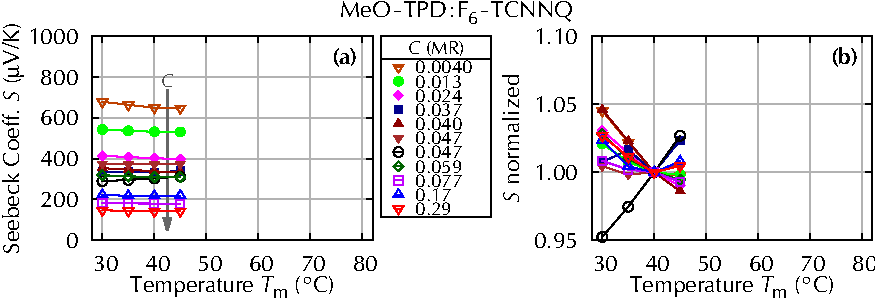
\includegraphics{plot/T-S-p1}\\%
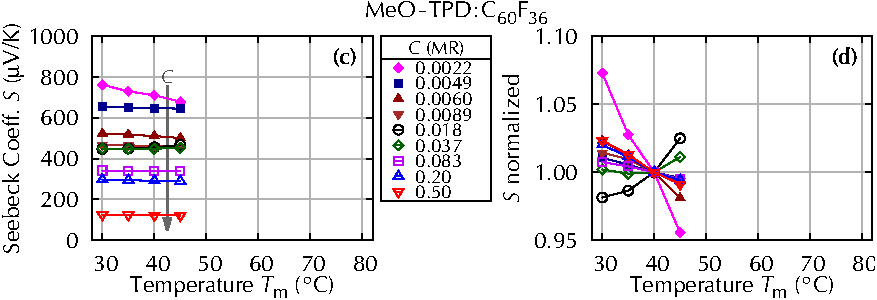
\includegraphics{plot/T-S-p2}\\%
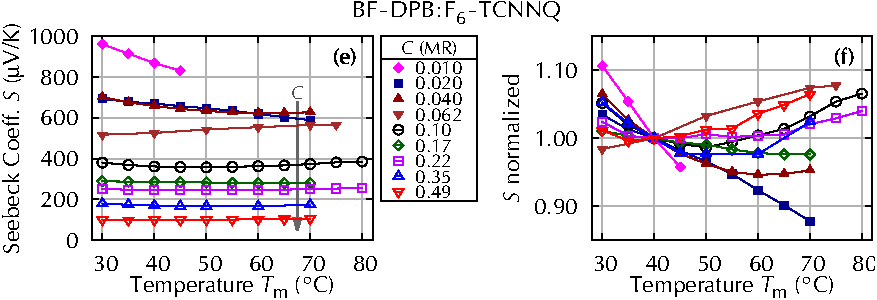
\includegraphics{plot/T-S-p3}\\%
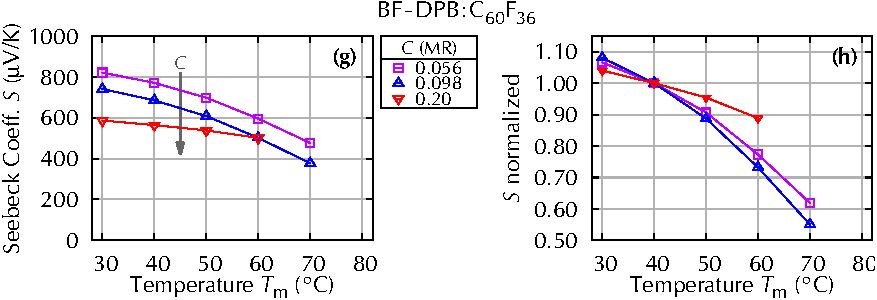
\includegraphics{plot/T-S-p4}\\%
\setcapwidth[c]{\tmCapWidth}%
\caption
[Temperature dependence of the Seebeck coefficient]%
{Temperature dependence of the Seebeck coefficient \S for four different material combinations,
left: absolute values,
right: normalized to the \Tm[40] measurements.
}%
\label{fig:T-S-p-all}
\end{figure}
%
%
Thermoelectric investigations at different temperatures are performed along with the conductivity experiments, similar to the studies of the n-doped samples. The resulting Seebeck coefficients \S at different temperatures are presented in \figref{T-S-p-all} for all four material combinations. As expected, all values of \S are positive in sign, thus holes are the dominating charge carrier species for all the p-doped samples. Electron conduction along the dopant molecules is not detected, not even for large \CLongs. The observed values for \S range from \uVK{100} to \uVK{1000} and a lowering of \S with rising \CLong is found. It was not possible to perform reliable Seebeck measurements on samples of \lili doped by \Ckl{0.030} of \CSF, as the resulting conductivities were below the resolution limit of the setup, as discussed in \secref{ExpResLimit}.

The samples with \meo as host material have only been measured in the range of \Tm[30] to \grad{45}, due to the low glass transition temperature of this material. Higher temperatures of up to \Tm[80] could be applied to the samples using \lili as host.
In order to investigate the influence of the temperature \Tm, the relative changes of \S, normalized to the value at \Tm[40], are depicted at the right hand side graphs in \figref{T-S-p-all}. A temperature of \grad{40} is chosen, as it is a device-relevant temperature and more stable to control than \Tm[30].

No clear trend of the temperature dependence of \S can be derived from the data. In the range of \Tm[30] to \grad{45} most samples vary by about $\pm5\,\%$.
This effect is much smaller than the influence a variation of the \CLong has.
The three samples of \lili doped by \CSF dramatically decrease in \S at elevated temperatures. This tendency is not present in the data of the other material combinations and is opposite to the results for n-doped \CS samples, where a gain of \S with temperature is found, as discussed in sections \ref{sec:ResPd-S-T} and \ref{sec:ResAS-S-T}. As a decreasing \S is correlated to an increasing \nhLong, the data of \lili doped by \CSF supports the theory of \CSF having a lower EA than the IEs of both hosts. Higher thermal energy allows to overcome the energetic difference and hence ionization of more and more dopants.

\subsection{Relation of Seebeck Coefficient to Doping Concentration}%
\label{sec:ResP-S-MR}
%
Comparing the Seebeck coefficients at one temperature of \Tm[40] for different \CLongs, a lowering of $\S$ with increasing \C is found for all four material combinations, ranging from \uVK{867} to \uVK{100}, as displayed in \figref{MR-See+Es-p-all}.
Using \eqnrefPage{S-Es-org}, the energetic difference \Es between the \EfLongL and the \EtLongL can be derived:
\begin{align}
 \Es =\S \cdot e \cdot \T \quad \text{ with } \quad\Es := \Ef - \Et
\PUNKT
\tag{\ref{eq:S-Es-org}}
\end{align}
\Es is given as the right hand axis in \figref{MR-See+Es-p-all}.
Following the trend of \S, the value of \Es decreases with increasing \C for both dopants, which is correlated to a shift of the \EfLong \Ef towards the \EtLong \Et. This finding is in agreement with the observations of the n-doped samples, where \Es drops with rising \CLong. No saturation is visible in the data and the samples of all four material combinations yield an almost linear relation of \S and \Es to the logarithm of \C.
%
\cBild[t]
{MR-See+Es-p-all}%
{Seebeck coefficient and derived \EsLong}
{Seebeck coefficient \S and derived \EsLongL at \Tm[40] for samples of \meo (triangles) and \lili (squares) doped by \FS (empty symbols) and \CSF (filled symbols).
}
%

The series of \meo doped by \FS starts at \C[0.004] with \Es[203]. This value is reduced to \Es[45] at \C[0.290], corresponding to a linear slope of \meV{88} per order of magnitude of \C.

Doping \meo by \CSF instead, a deviation from a linear relation is present between $\C[0.006]$ and \mr{0.018}. Overall the slope is determined to \Es[67] per order of magnitude of \C and therefore somewhat lower than for the use of \FS as dopant.

In case of \lili doped by \FS, the values for \Es at low \C are larger than observed for \meo as host material. At \Cgr{0.100} a reasonable agreement is found. The overall linear slope is \meV{142} per order of magnitude, being the highest of all four material combinations.

For the three reliably measurable samples of \lili doped by large concentrations of \CSF, the highest values of all four material combinations in the corresponding \C-regime are measured, with a maximum of \Es[241] at \C[0.056]. Here the slope is \meV{118} per order of magnitude of \C.

In conclusion, the samples of all four material combinations yield the same trend of a linear reduction of \S and \Es with increasing logarithm of \C.
Comparing the hosts, samples of \lili have larger values of \S and \Es and stronger slopes compared to samples of \meo. The larger values are in agreement with \lili having a larger IE than \meo, making electron transfer to the dopant less probable and therefore generating a lower \nhLong at the same \CLong for each dopant. This results in a greater energetic difference between \EfLong and \EtLong and thus a larger value of \S and \Es, particularly for doping by \CSF.
The strong slope of \S and thus \Es observed for \lili as host is attributed to filling of the tail states of the host's \dosLong that leads to a rapid shift of \Ef. At high \CLongs of \FS, a reduced slope is found, comparable to the samples of \meo.

Concerning the dopants, \FS leads to a lower value of \S and \Es and to a larger slope with \C than \CSF. The lower values of \S and \Es indicate a higher doping efficiency of \FS compared to \CSF. This finding supports the above proposed theory of \FS having a larger EA than \CSF, contrary to the literature values.

Comparing the results to the n-doped \CS samples of the previous chapters, larger values of \S and \Es are detected for the p-doped samples at low \CLongs.
This can be understood from the fact that the amorphous hosts investigated in this chapter are expected to have broader \dosLongs compared to the polycrystalline \CS. A broader host's \dos leads to a larger fraction of host molecules having a larger IE than the EA of the dopant and hence doping these molecules is less probable. Consequently, the \nhLong is lower which results in a larger \S and \Es.

\subsection{Comparison of Seebeck Energy and Activation Energy}
\label{sec:ResP-EsEact}

\cBild[b]{MR-Es+Eact-p}%
{Comparison of \Es and \Eact}
{Comparison of \EsLongL and \EactLongL for four different material combinations. \Es is probed at \Tm[40], \Eact is fitted from conductivity data presented in \figref{T-Cond-p}.}

In \figref{MR-Es+Eact-p}, \Es is compared to the previously discussed \EactLong \Eact, for the four different material combinations. All samples show an \Es that is approximately \meV{100} lower than \Eact. Such a large difference is not observed for the n-doped samples discussed in the previous chapters. In case of \CS n-doped by the air-sensitive dopants \CrPd and \WPd, a difference of only \meV{25} to \meV{75} is found at \Cgr{0.100}. That observation is attributed to a disturbance of the morphology by the large number of dopant molecules and hence a decreasing mobility with increasing \C, as discussed in \secref{ResPd-EsEact}.

\cBild[t]{MR-Eact-Es-p}%
{Difference between \Eact and \Es}
{Difference between \EactLongL and \EsLongL for samples of \meo (triangles) and \lili (squares) doped by \FS (empty symbols) and \CSF (filled symbols).
}

In order to investigate the difference of \Es and \Eact more closely, this quantity is plotted in \figref{MR-Eact-Es-p}.
Three of the four material combinations are in good agreement, only the three samples of \lili doped by \CSF show a difference that is smaller by $\approx\meV{50}$. The calculated differences range from \meV{100} to \meV{200} with one value as high as \meV{241}.
All material combinations yield a rising difference with \C at low \C.
Doping both hosts by \Cgr{0.050} of \FS, the difference between \Es and \Eact is found to be constant at a similar value around \meV{175}. This suggests that for all these samples the mobility has the same dependence on the temperature, compare \eqnrefPage{mob-von-Eact-Es-org}.

Samples doped by \CSF show a further increasing difference at larger \C, due to a faster decreasing \Es than \Eact at these \CLongs.
The slower drop of \Eact with \C at high \C of \CSF is attributed to thermal activation of dopants, due to the expected low EA of \CSF in respect with the IEs of the hosts as discussed in \secref{ResP-CondEact}. This model is supported by the temperature-dependent Seebeck experiments on the samples of \lili doped by \CSF, where a strong reduction of \S with increasing \T at high \C is observed, compare \figref{T-S-p-all}~(h).

\section{Degradation}\label{sec:ResP-Degradation}
%

In this section, the effect of elevated temperatures on p-doped layers is studied by conductivity investigations. Three samples of different material combinations are investigated. In order to compare the data, the conductivity of each sample is normalized to the value at \T[25], and depicted in \figref{killing-MeO}. The \cLong is measured twice with a delay of 30~minutes to 1~hour for most temperatures, which allows for detection of sample degradation. As reported in \secref{ResP-CondEact} for all samples at low \T, an increase of \c with \T is visible.

\cBild[t]
{killing-MeO}
{Degradation induced by heating}
{Degradation induced by heating for three different material combinations. The conductivity is normalized to the value at \T[25].}

The sample of \meo doped by \FS (at \C[0.040]) shows a slight degradation starting at \T[65]. A single measurement at \T[80] yields a maximum of \c, followed by a rapid decrease. The degradation is attributed to the glass transition of \meo (\Tg[67]\cite{Thelakkat1998}).

Doping \meo by \CSF (at \C[0.023]) a different tendency is found.
Between \T[70] and \grad{80} a sudden gain of \c by a factor of more than 3 is observed. 37~minutes later, at the same temperature, \c changes only by 1\,\%, so no degradation is visible at \T[80]. At \T[90] the sample is degrading rapidly. 
This data indicates that the presence of \CSF might shift the glass transition temperature of \meo upwards. Furthermore, it seems evident that thermal annealing raises the doping efficiency of \CSF in \meo.
As \CSF has been reported\cite{Mao2013} to thermally decompose at \T[120]\footnote{on indium tin oxide (ITO) substrates}, it is possible that in \meo the dopant decomposes as well. This could lead to a donation of strongly electronegative flour atoms to the host that would work as additional p-dopants and strongly increase the \nhLong.

Using \lili as host and \FS as dopant (at \C[0.100]), a higher thermal stability is found. Starting at $\T[65]$ a slow degradation of \c is observed, but up to \T[100] the effect is much lower than the gain due to the rising temperature. At $\T{}\geq\grad{115}$ a strong degradation is present.

No degradation is studied for \lili doped by \CSF.

\pagebreak
\section{Conclusion} \label{sec:ResP-Conclusion}
Comparing the host materials when using the same dopant, the samples of \meo show higher conductivities than samples of \lili, often by more than one order of magnitude. This trend is particularly interesting, as for both materials a similar OFET-mobility has been measured. Hence, the larger conductivity for \meo is attributed to a larger \nhLong due to the lower \IE compared to \lili.
The \EactLong is lower for \meo samples compared to \lili, but the difference decreases with increasing \CLong. A similar tendency is observed by the Seebeck investigations, showing that the Seebeck coefficients and hence \Es are larger for \lili, again with a decreasing difference with increasing \CLong.
These larger values obtained for \lili are in agreement with it having the larger IE, making electron transfer to the dopant less probable and therefore leading to a lower \nhLong compared to \meo. The strong slope of \S and hence \Es, observed for \lili as host is attributed to filling of tail states of the \dosLong.
Finally, it is evident that \lili has a higher thermal stability than \meo, which degrades already at \T[80].

Comparing the dopants in the same host material, higher conductivities are obtained for using the lighter \FS than for \CSF. This trend shows that \FS has a larger EA than \CSF, opposite to the estimated literature values\cite{Tietze2012,Meerheim2011}. For \FS, an EA larger and for \CSF an EA lower than \eV{5.2} is expected, as the IE of \lili is \eV{5.23} and only the former is able to dope it well.
The \EactLongs suggest a thermally induced ionization for large concentrations of \CSF, leading to higher \nhLong at elevated temperatures.
Seebeck measurements yield that in \meo, both dopants result in similar \S and hence \Es. At large \C, samples of \FS yield somewhat lower values compared to \CSF. In samples of \lili doped by \CSF much larger \S are found compared to doping by \FS. This suggests that \CSF generates a lower \nhLong in \lili, in agreement with its above discussed expected low EA. Temperature-dependent Seebeck studies show that for this material combination at elevated temperatures the resulting values of \S strongly decrease, supporting the model of thermal induced dopant ionization.

Most material combinations yield a strongly superlinear increase in \cLong with \CLong, opposite to the n-doping experiments of the previous chapters, where mostly linear relations are found.
Here, only for the combination of doping \meo by \CSF in the medium doping regime a linear relation is observed. In general, the host \lili and the dopant \FS lead to stronger slopes than the other materials.
%
While samples using \CSF yield a reduced slope at elevated \CLongs, samples doped by \FS continue to show strongly increasing \cLongs. Seebeck studies of samples doped by \FS show a rapid drop of the Seebeck coefficient in the medium doping regime indicating an increasing doping efficiency.
%
The comparison of conductivity and Seebeck investigations of samples of \meo doped by \CSF indicate that the decreasing slope of $\c(\C)$ at elevated \C is most likely due to a reduction of the mobility, since the Seebeck coefficient and hence the \nhLong is not saturating. This reduction is attributed to a disturbance of the layer morphology by the heavy dopant molecules. Analogously, the decreasing \c-slope of samples of \lili highly doped by \CSF is explained.

Overall, for devices the combination of the more stable host \lili with the stronger dopant \FS is advised.
In a future work the higher fluorinated compound C$_{60}$F$_{48}$ should be investigated, since it has been reported to have a larger EA than \CSF\cite{Liu1997} due to the increased amount of electron attracting fluorine atoms and has been shown to be electrically stable even upon twofold ionization\cite{Jin1994}.


\cleardoublepage
%äöüß
\chapter{Pentacene p-Doped by \FV}\label{chap:P5}
\addcontentsline{lof}{chapter}{\thechapter\hspace*{1ex} Pentacene p-Doped by \FV}

%
\intro{After studying two amorphous organic hole transporters in the previous chapter, the high mobility prototypical polycrystalline organic material \pen is investigated in the following. \FV is chosen as p-dopant, since it has almost the same size and weight as \pen and is expected to neatly integrate into \pen layers at low \CLongs.
Theoretical studies predict an increasing doping efficiency with \CLong for this material combination, which is experimentally tested in this chapter.
}

\newpage
%
The combination of \pen doped by \FV has been studied earlier by several groups and techniques. AFM surface scans have shown that layers of \pen can be grown highly crystalline and that at very low \CLong, \FV does not disturb the molecular order of \pen\cite{Ha2009}. Increasing the \CLong, the crystallite size has been found to decrease and rough surface structures have been reported\cite{Kleemann2012a}.
Details about the materials are summarized in the materials \secref{Mat}.

Theoretical studies on this model system of \pen doped by \FV, with similar-sized dopant and host, suggest\cite{Mityashin2012a} that for \OSCs, a certain threshold \CLong exists, below which doping does not increase the conductivity. This threshold is attributed to electron--hole attraction hindering the charge pair dissociation. Increasing the \CLong \C, the potential landscape of the \IE IE is expected to be altered such that percolation pathways for dissociation are generated. Hence, the doping efficiency is expected to increase with \C.
%
To test this model, conductivity and Seebeck investigations are performed.

\section{Conductivity Changes after Preparation}%
\label{sec:ResP5-LongTimeCond}
In an analogous way to the previously investigated materials, the change of conductivity of freshly produced \nm{30} thick layers over time is investigated before reporting on the observed conductivities.
%
\cBild[b]
{MR-LongTimeCond-P5}
{Conductivity change during first hour after preparation, fitting parameters}
{Conductivity change during the first hour after sample preparation for \pen doped by \FV. Fitting parameters, according to \eqnrefPage{LongTimeCond-exp}.
}
%
As for most sets of materials, the conductivity of each sample is continuously probed \insitu for 1~hour at a fixed temperature of \T[25], as discussed in detail in \secref{ResPdLongTimeCond}. A strong reduction of conductivity \c over time is detected for most samples of \pen doped by \FV. To quantify the change in conductivity, the data are fitted according to \eqnrefPage{LongTimeCond-exp} and a good agreement with the fit function is found for most samples. The resulting fitting parameters are presented in \figref{MR-LongTimeCond-P5}.

The strongest reduction is determined for the lowest doped sample, resulting in a fitted maximal relative change $\chi$ of $-50\,\%$ of the initial value of the conductivity. Samples of higher \CLongs show smaller decreases and two samples (\C[0.043] and \mr{0.066}) even a slightly increasing \cLong over time. The highest doped sample of \C[0.193] shows again a strong reduction.

The time constant $\tau$ scatters around \SI{30}{\minute} for all samples, being comparable to the results for \CS n-doped by \dmbi (compare \figrefPage{MR-LongTimeCond-n-AS-fitparameter}).

\section{Relation of Conductivity to Doping Concentration}%
\label{sec:ResP5-CondMR}
%
\cBild
{MR-Cond-P5}
{As-prepared conductivity}
{As-prepared conductivity \vs \CLong of layers of \pen doped by \FV, probed at \T[25], directly after sample preparation (full circles) and after thermal annealing (open circles). Literature values taken from Harada\etal\cite{Harada2010} and Kleemann\etal\cite{Kleemann2012a} are added for comparison.
Dashed lines are linear fits with slopes 1.0 and 2.5.
}

Measured directly after sample fabrication at \T[25], the detected conductivities are in the range of \c[5.8E-3] to \Scm{3.7E-2}, and a sublinear (slope $< 1.0$) increasing with \CLong up to \mr{0.080}, followed by a decrease at higher \C is found, as shown by the full circles in \figref{MR-Cond-P5}.
The sublinear rise of $\c(\C)$ suggests a reducing charge carrier mobility with increasing \CLong and hence a compensation to the gain of \nhLong induced by the dopants. This decrease of the mobility is attributed to a disturbance of the polycrystalline morphology of \pen by the rising number of dopants, as reported in literature\cite{Kleemann2012a}.

As described in the previous section, the \insitu conductivity strongly changed after sample fabrication. To reach stable measurement conditions, the samples were thermally annealed for 1~hour at \T[70] prior to further investigations. Afterwards, the conductivities are measured again and found to be constant over time, thus the heating seems to accelerate and saturate the effect responsible for the change of the \cLong over time. The values are displayed by the open circles in \figref{MR-Cond-P5}. It can be seen that the heat treatment changes the room temperature conductivity in the same direction as the trend of the continuous investigations after sample preparation indicated.
The conductivity of the lowest doped sample drops by two orders of magnitude, whereas samples of higher \CLongs show less reduction. Only the \cLong of the sample of \C[0.043] increased slightly after heating. Two samples with higher \CLongs show almost constant \cLongs and the highest doped sample decreased by almost one order of magnitude, in agreement with the tendency of the continuous measurements directly after sample fabrication.

After thermal annealing, the \cLong has a strong \C-dependency in the low to medium doping regime. A strongly superlinear rise with a slope around 2.5 in this double-logarithmic plot is found for the four lowest doped samples, as indicated by the dashed line in \figref{MR-Cond-P5}. Similar slopes are determined for \meo and \lili p-doped by \CSF in \secref{ResP-CondMR}, but at large \CLongs.
%
The strong change of the \cLong directly after fabrication as well as after thermal annealing is either attributed to changes of the mobility or to changes of the \nhLong, for example by diffusion and agglomerating or re-evaporation of the light diffusive dopant \FV, having a sublimation temperature in the range of \Tdep[100]. As this effect has a \C-dependency, it might be responsible for the superlinear rise of $\c(\C)$ as well.
The changes of the \cLong are smallest for samples of \CLongs between \C[0.043] and \mr{0.066}, indicating that \FV is best integrated into the layer of \pen in this range of \CLong.

Interestingly, the conductivity values as well as their slope prior to annealing are in good agreement with investigations published by Harada\etal\cite{Harada2010}, whereas after heating they agree to experiments by Kleemann\etal\cite{Kleemann2012a}. Both sets of data are shown in \figref{MR-Cond-P5}, with the authors' kind permissions.
%
Harada\etal have reported\footnote{Personal correspondence with the author.}
that they observed a decreasing conductivity after sample processing as well. They decided to measure conductivity and Seebeck coefficient as quickly as possible, instead of performing a thermal annealing step as done here. This explains why their conductivity data are in agreement with the above discussed measurements prior to heat treatment. Kleemann\etal on the other hand used samples that where in contact with air for 30~minutes after fabrication. Thus, this suggests that air-exposure has a similar influence on the conductivity of these samples than thermal treatment. It is possible that the light and volatile \FV molecules desorb from the layer upon contact with air or during heating in vacuum.

Both studies have presented \C-dependent OFET-mobility measurements in addition to \cLong studies and reported a similar trend of a slowly decreasing OFET-mobility at low \C, followed by a significant decrease at \Cgr{0.050}. Hence, the drop of \c at high \C detected in all four experiments and shown in \figref{MR-Cond-P5}, is explained by a decreasing mobility.
Due to very narrow contact distances and thus high fields in an OFET geometry, it is expected that the \nhLong is strongly enhanced and hence compensates for dopant induced traps. Thus, in conductivity geometry a different tendency of the mobility, especially for low \CLongs, is expected.

\section{Comparison of Seebeck Energy and Activation Energy}
\label{sec:ResP5-EsEact}

\cBild[b]
{MR-Es+Eact-P5}
{Comparing \Eact and \Es}
{Comparing \EactLong \Eact and \EsLong \Es. \Eact is fitted from conductivity data of \T[25] to \grad{70}, \Es is measured at \Tm[40]. Literature values for \Es taken with kind permission from Harada\cite{Harada2010} are added for comparison.
}

Temperature-dependent conductivity investigations in the range of \T[25] to \grad{70} on this material system allow to derive an \EactLongL for each sample, using \eqnrefPage{CondActivation}. The derived \Eact is depicted in \figref {MR-Es+Eact-P5} and found to strongly vary with \CLong, with a maximum of \Eact[357] at \C[0.011]. The obtained trend of $\Eact(\C)$ is almost inverse to the tendency of the $\c(\C)$ after thermal annealing. Samples of high \c show low values of \Eact and vice versa, in agreement with the data presented in the previous chapters and only the lowest doped sample deviating.

Besides conductivity investigations, Seebeck measurements at \Tm[40] (after thermal annealing) are performed on this material system as well, allowing to derive the energetic difference \Es between \EfLongL and \EtLongL.
\Es is positive for all samples, as expected for p-doped layers and the values are presented in \figref{MR-Es+Eact-P5} where they are compared to \Eact.
The highly doped samples yield a slowly decreasing $\Es(\C)$, in the range of \Es[103] to \meV{73}, whereas for the lowest doped sample the Seebeck measurement was not successful.
This rather small \Es at low \C indicates a high doping efficiency of \FV in \pen. Another explanation for the low \Es is that intrinsic \pen has been reported to have an extremely narrow \dosLongL with a Gaussian width in the range of only \gausswidth[70]\cite{Yogev2011}. Such a narrow \dos requires a small \Es to generate free charges.
Upon doping, the width of the \dos and hence \Es are expected to rise due to molecular disorder. This effect is not visible in the data and might be compensated by the increasing \CLong, resulting in an almost constant \Es.

The differences between \Es and \Eact for most samples are attributed to a thermal activation of the mobility, as discussed in \secref{ResPd-EsEact}. This contribution is strongest for the sample of \C[0.011] and decreasing with \C. As in the same \C-regime, a superlinear rise of $\c(\C)$ is observed and \Es is almost constant, the decreasing thermal activation of the mobility seems to be correlated to a mobility rise in this regime of \C.

Harada\etal\cite{Harada2010} have performed Seebeck measurements on \pen doped by \FV as well, but at lower \Tm[24] and without thermal annealing the samples. Their data are included in \figref{MR-Es+Eact-P5}.
An almost identical value of \Es is measured at \C[0.020] in both setups: Harada reported \Es[81.7] (\S[275.0] at \Tm[24]), compared to \Es[82.2] (\S[262.5] at \Tm[40]) measured in our setup.
At higher \CLongs, the two experiments differ, with Harada's values being lower.
The deviation of the two experiments is attributed to the fact that Harada did not anneal the samples prior to Seebeck investigations, as discussed above. Thus, this deviation is an indication for heating or air-exposure of highly \FV-doped \pen samples reducing the \nhLong, most probably by the agglomeration or re-evaporation of the diffusive \FV molecules. At low \CLongs, where the two Seebeck measurements are in agreement, the \nhLong seems not to be affected by thermal annealing and therefore the different conductivities are attributed to changes in the mobility induced by morphological changes in the layer and accelerated by the heat treatment.
%
Re-evaporation of dopants is not likely to be present in the data at low \C, since this would correspond to a shift of \Es to smaller \CLongs, flattening the curve even more.

\section{Conclusion}
%
The strong reduction of the \insitu \cLong over time, which could be accelerated and saturated by heat treatment, is attributed to morphological changes in the layer, reducing the mobility. A decreasing \cLong at high \CLongs is in agreement with a strongly reduced OFET-mobility reported in literature\cite{Harada2010,Kleemann2012a}.
%
The rather small \Es at low \CLongs indicates a high doping efficiency of \FV in \pen and/or a narrow \dosLong. At higher \CLongs the \Es is found to be almost constant, but larger than obtained for highly n-doped \CS samples, which is attributed to a broadening of the \dosLong, partly compensated by the increasing \CLong.
A comparison with literature values of unannealed samples suggests that at \Cgr{0.020} during thermal treatment, re-evaporation of the light and diffusive dopant molecules occurs.

% Model of Mityashin2012a
Neither the presence of a threshold \CLong for the generation of free charge carriers nor indications for an increasing doping efficiency upon rising \CLong, as predicted by Mityashin\etal\cite{Mityashin2012a}, are observed by the measurements.
Rather high conductivities directly after sample fabrication, showing only a moderate increase with \C, even contradict this model. Seebeck measurements do not show indications for an increasing doping efficiency with \C, which would be correlated to a more rapid decrease of \Es.
It is possible that the predicted phenomena are concealed by morphological effects or that they occur at lower \CLongs.

\cleardoublepage
%äöüß
\chapter{Estimating the Doping Efficiency and the Mobility}\label{chap:Rech}
\addcontentsline{lof}{chapter}{\thechapter\hspace*{1ex} Estimating the Doping Efficiency and the Mobility}

%
\intro{Following four experimental chapters, a theoretical model for deriving trends for the \nLong, the doping efficiency as well as the charge carrier mobility from conductivity and Seebeck data is developed and is first applied to data of n- and later to p-doped samples.
In \secref{rechMobLL}, a lower limit for the charge carrier mobility is derived from \cLong measurements. Afterwards, in \secref{rechDopEffLL} a similar estimation is performed for the \nLong and the doping efficiency.
Supporting these findings by Seebeck data, the physically allowed position of the \EtLong is narrowed down in \secref{rechConclSeebeck}. This leads in \secref{rechConstEt} to the assumption of a constant \EtLong for all n-doped samples, allowing to derive absolute values for the above mentioned parameters of each sample. Finally, in \secref{rechApplyForP} the developed model is applied to data of p-doped samples.
This chapter is finalized by a conclusion in \secref{rechConclusion}.
}

\newpage

\section{Lower Limit of the Mobility}\label{sec:rechMobLL}
%
\cBild[b]
{sim_H+D-vs-MR}
{Relation of \CLong to densities of host and dopant molecules}
{Influence of doping concentration \C on densities of host \nH and dopant \nD molecules, calculated via equations \eqref{nHD} on page~\pageref{eq:nHD}. Values given as a fraction of the total density of molecules $\nM=\nH+\nD$.}
%
In this first section a lower limit for the charge carrier mobility \mobLL is derived from conductivity measurements.
Assuming a \C-independent and constant doping efficiency \DopEff, the \nLong \neh directly follows the trend of the \nDLongL for varying \CLong, illustrated in \figref{sim_H+D-vs-MR}, and can be calculated by \eqnrefPage{CCD-from-DopEff}:
% %
\begin{equation}
\neh = \DopEff \cdot \nD = \DopEff \cdot \nM \cdot \frac{\C}{1+\C} \label{eq:CCD-from-DopEff-calc}
\PUNKT
\end{equation}
%
This calculated value of \neh can be correlated to the charge carrier mobility \mobeh for a measured conductivity \c as
\begin{align}
\mobeh &= \frac{\c}{e \cdot \neh} \label{eq:Cond-CCD-Mob-calc} \\
\Rightarrow\mobeh &= \frac{\c}{e \cdot \DopEff \cdot \nM} \cdot \frac{1+\C}{\C}
\label{eq:mob-von-DopEff+C}
\PUNKT
\end{align}
Above equations show that for a given (measured) conductivity, the estimated mobility is inversely proportional to the estimated \neh and thus the \DopEff. Consequently, by measuring \c and assuming the maximum possible doping efficiency of \DopEff[100], meaning each dopant molecule is ionized and provides one free charge carrier, the lower limit of the mobility~\mobLL can be derived:
\begin{equation}
\mobLL = \frac{\c}{e \cdot 100\,\% \cdot \nM} \cdot \frac{1+\C}{\C}
\label{eq:mobLL}
\PUNKT
\end{equation}

\cBild{calc-MobLL-n}
{Lower limit of mobility for n-doped \CS}
{Lower limit of the charge carrier mobility \mobLL for n-doped \CS, calculated by \eqnref{mobLL} using measured conductivity data, probed at \T[40].}
%
In \figref{calc-MobLL-n}, this calculation is performed for the n-doped \CS samples presented in chapters~\ref{chap:PaddleWheels} and \ref{chap:AirStables}, using four different n-dopants. Here, the conductivity measured at a temperature of \T[40] (after thermal annealing) is used, as this data will later be compared to Seebeck studies performed at \Tm[40].
%
The lower limit of the mobility \mobLL is found to be highest for the dopant \CrPd with a maximum of \mobLL[0.90] for \C[0.005].
Record values of the mobility of undoped \CS layers in the order of \mob[5] are found in the literature\cite{Itaka2006}\footnote{measured in an OFET geometry on a monolayer of \pen}.
At \CLongs of \Ckl{0.045}, \mobLL is rather constant for \CrPd with values in the range of \mobLL[0.50], whereas at higher \C the \mobLL drops significantly.
A similar trend is found for the second air-sensitive dopant \WPd. Below \C[0.150], almost constant values in the range of \mobLL[0.15] are derived, followed by a drop for higher \CLongs.
This drop of the \mobLL suggests a disturbance of the morphology by the large amount of heavy dopants in the layer and hence a reduction of the real mobility.

A different relation is found for the lighter air-stable dopants, \aob and \dmbi. The samples doped by \aob yield an almost constant lower limit of the charge carrier mobility in the order of only \mobLL[9E-3].
Samples doped by \dmbi have a \mobLL that is as small as for \aob for the lowest \C, but strongly increasing with \C. A saturation value around of \mobLL[0.1] is observed, being even higher than for the air-sensitive dopants at these \CLongs.

\Figref{calc-MobLL-n} shows that the materials which yield a linear relation of $\c(\C)$ at low \CLongs (compare \figrefPage{MR-Cond-n-PdvsAS}) have a \C-independent \mobLL.
It is expected that for low \CLongs the mobility is the same for each dopant, therefore the different and almost constant values of the \mobLL indicate different doping efficiencies of the dopants, which is addressed in the next section. As the \cLongs of samples of \CS doped by \dmbi increase superlinearly with \CLong, this effect can most probably be attributed to an increasing \DopEff with \C for this dopant, as discussed in \secref{ResASCondMR}.
From this simple model it cannot be distinguished whether the observed decrease or saturation of the \mobLL at high \C for \CrPd, \WPd and \dmbi are correlated to trends of the real mobility or a decreasing \DopEff.

\section{Lower Limit of the Doping Efficiency}\label{sec:rechDopEffLL}
Besides estimates for the lower limit of the mobility by assuming \DopEff[100], as done in the previous section, the opposite approach can be performed by assuming a constant mobility. If the highest measured literature value for the mobility \mobUL of the host material is chosen, a lower limit of the \nLong \nehLL and doping efficiency \DopEffLL can be derived:
\begin{align}
\nehLL &= \frac{\c}{e\cdot\mobUL} \label{eq:nehLL}\\
\DopEffLL &= \frac{\c}{e \cdot \mobUL \cdot \nM} \cdot \frac{1+\C}{\C} \label{eq:DopEffLL}
\PUNKT
\end{align}
As the real mobility in the used sample geometry is expected to be lower than this record value \mobUL and furthermore is expected to be negatively affected by the introduction of dopant molecules disturbing the morphology, the real values of \neh and \DopEff must be larger than \nehLL and \DopEffLL to fulfill \eqnref{mob-von-DopEff+C}.

In case of \CS, the maximum reported value is in the order of \mob[5]\cite{Itaka2006}, measured in an OFET geometry.
This value can be interpreted as an upper limit \mobUL, because OFET experiments usually overestimate the charge carrier mobility in comparison to conductivity measurements, as discussed in \secref{ResPd-EsEact}. In an OFET geometry the free charge carriers are generated by the field induced by the gate voltage and their number typically is much larger than values achieved by doping. As the mobility of an \OSC usually increases with charge carrier density, OFET channel mobilities are generally larger than the mobilities in the bulk material and hence in the conductivity geometry.

\cBild[t]
{calc-CCDLL+neLL-n}
{Lower limits of \neLong and doping efficiency for n-doped \CS}
{Lower limits of (a) \neLong \neLL and (b) doping efficiency \DopEffLL for n-doped \CS, calculated by assuming a constant mobility set to the record value for intrinsic \CS of \mob[5]\cite{Itaka2006} and using measured conductivity data, probed at \T[40].}%

The lower limit of the \nLong \neLL is calculated for the n-doped \CS samples discussed in chapters~\ref{chap:PaddleWheels} and \ref{chap:AirStables}, again using the conductivity measured at a temperature of \T[40]. The results are depicted in \figref{calc-CCDLL+neLL-n}\,(a) and found to be largest for samples doped by \CrPd and lowest for \aob, as expected from the estimates for \mobLL in the previous section. All material combinations show an increase of \neLL with \CLong, with a saturation and a decrease observed for high concentrations of the two air-sensitive dopants, \CrPd and \WPd. If this decrease in \neLL is present in the real values of \ne as well, and not an artifact produced by the assumption of a constant mobility, the reason most probably is agglomeration and thus shielding of dopants. The highest \neLL close to $\SI[per-mode=reciprocal]{E19}{\per\cubic\centi\meter}$ are obtained for \CS highly doped by \dmbi, \CrPd or \WPd, whereas for \aob the largest value is one order of
magnitude lower. These obtained values have to be seen in relation to the density of molecules of \CS of \mbox{$\nM{}_{\text{,C}_{60}}=\SI[per-mode=reciprocal]{1.36E+21}{\per\cubic\centi\meter}$} calculated via \eqnref{nM-from-MatPara} using the material parameters from \tabrefPage{MatProp}.

Knowing \neLL, the lower limit of the doping efficiency \DopEffLL for each sample is calculated using \eqnref{DopEffLL} and the results are presented in \figref{calc-CCDLL+neLL-n}\,(b). As mobility and doping efficiency are inversely proportional, the trends of the curves for \DopEffLL correspond to the trends of the lower limits of the mobilities \mobLL, presented in \figref{calc-MobLL-n}. \CS doped by \CrPd leads to a maximum value of \DopEffLL[18] at \C[0.005] and an almost constant \mbox{$\DopEffLL\approx10\,\%$} up to \C[0.045], followed by a decrease. Samples comprising \WPd yield efficiencies around \DopEffLL[3] and a drop at $\C>\mr{0.147}$.
\aob-doped samples have the lowest \DopEffLL of around \DopEffLL[0.2] and \dmbi samples start at a similar value, rising by a factor of 10 to a saturation around \DopEffLL[2] at high \CLongs. The gain in \DopEffLL for low \C of \dmbi samples is most probably correlated to an increasing real \DopEff in this range, as it is not unlikely that only for one dopant the mobility of \CS is rising with the \CLong.

At low \CLongs, the real mobilities of all four material combinations are expected to be least affected by the dopants and are consequently similar. Therefore, the calculated \DopEffLL at low \C can be directly compared and should be correlated to the real doping efficiency \DopEff by the same constant factor for all four combinations. This factor is given by the ratio of the used record mobility of \mob[5] and the real value of the bulk material in this sample geometry. Hence, at low doping concentration the real doping efficiency \DopEff of \CrPd is approximately 3~times higher than for \WPd and around 15~times larger than for both air-stable compounds.

\section{Conclusions from Seebeck Measurements}\label{sec:rechConclSeebeck}
%
The \nLong \neh is correlated to the density of dopant molecules~\nD via the doping efficiency \DopEff, see \eqnref{CCD-from-DopEff-calc}. On the other hand, \neh can be calculated by solving the integral of the product of \dosLong $\dos(E)$ and \fFDLong $\fFD(E,\Ef)$ over all energies, as demonstrated in \eqnrefPage{CCD-basic-integral}. Thus, for a known $\dos(E)$ and given \DopEff, the position of the \EfLongL can be derived by shifting \Ef until this condition is fulfilled:%
\footnote{Here, for holes $\fFD(E)$ instead of $1-\fFD(E)$ is used as well, as for p-conduction the corresponding \dos is switched from LUMO to HOMO.}
\begin{align}
\neh &= \DopEff \cdot \nD
=
\int_{-\infty}^\infty
\dos(E)
 \cdot
\fFD(E,\Ef)
 ~ dE
\PUNKT
\intertext{Using a Gaussian density of states and setting its maximum to $\gausscenter=0$ this becomes:}
\neh &= \DopEff \cdot \nD
=
\int_{-\infty}^\infty
%\dos(E)
\frac{\nH}{\sqrt{2 \pi} ~ \gausswidth} \exp{-\frac{E^2}{2\gausswidth^2}}
 \cdot
%f(E,T)
\frac{1}{1+\exp{\frac{E-\Ef}{\kT}}}
 ~ dE
\label{eq:Ef-vonDopEff}
\PUNKT
\end{align}
With \nH and \nD being the densities of host and dopant molecules that can be calculated from the \CLongL via equations~\eqref{nMHD} and \eqref{C}.
Iterative numerical calculations allow to derive \Ef for varying \C and \DopEff, which is plotted in \figref{calc-Ef-von-DopEff} for n-doping using a \C-independent \dos of width \gausswidth[100] (sketched in \figref{calc-Ef-von-DopEff}) and setting \T[40]. As the doping efficiency cannot exceed \DopEff[100], only values above the solid line corresponding to the \Ef at \DopEff[100] are physically allowed. It can be seen that with increasing \C the \Ef reaches densely populated regions of the \dos, when assuming a constant \DopEff.

%
\cBild[p]
{calc-Ef-von-DopEff}
{Calculated \EfLong position for varying \CLong and \DopEffLong}
{Calculated \EfLong position $\Ef(\C)$ for different doping efficiencies \DopEff using \eqnref{Ef-vonDopEff} for a Gaussian \dos with \gausswidth[100] and \T[40]. Only values in the gray area are physically allowed with $\DopEff\leq100\,\%$.
}
\cBild[p]
{calc-ETr-von-Es+DopEff}%
{Calculated \EtLong position for measured \Es and varying \CLong and \DopEffLong for n-doped \CS}%
{Calculated \EtLong position \Et with respect to the maximum of the Gaussian \dosLong for measured \Es and varying \CLong and \DopEff for n-doped \CS samples. Parameters used: \gausswidth[100] and \T[40]. The gray area corresponds to the physically allowed range between lower and upper limit of the doping efficiency.
}

% \subsection{Application to Data}
The approach presented above of deriving the position of \Ef for a given doping efficiency \DopEff is now combined with the data of the Seebeck studies to calculate the absolute position of the \EtLong \Et. Via Seebeck investigations the energy difference \Es between \Ef and \Et at a certain \CLong is derived, which is subtracted from a calculated \Ef for a given \DopEff at the same \C, yielding the position of \Et:
\begin{equation}
\Et = \Ef-\Es \tag{\ref{eq:Es=Ef-Et}}
\PUNKT
\end{equation}
\Figref{calc-ETr-von-Es+DopEff} shows the resulting \Et for the data of the studied n-doped \CS layers.
%
In this calculation the width of the Gaussian \dos is set to \gausswidth[100] for all \C, which is chosen to be somewhat higher than the reported \gausswidth[88]\cite{Fishchuk2010} for undoped \CS to compensate the influence of doping that is expected to broaden the \dos.
As the doping efficiency is required to be greater than the above derived lower limit \DopEffLL and cannot exceed \DopEff[100], only a certain region of \Et is allowed, marked by the filled areas in \figref{calc-ETr-von-Es+DopEff}. This physically possible region is for most samples between \meV{-300} and \meV{-100} with respect to the maximum of the Gaussian density of states. It is narrowest for \CrPd, due to the large value obtained for \DopEffLL.

\section{Assuming a Constant Transport Level}\label{sec:rechConstEt}
%
%
\cBild[b]
{calc-Es-von-DopEff}
{Measured and calculated \EsLong for varying \CLong and \DopEffLong at constant \Et for n-doped \CS}
{Measured \EsLong \Es for n-doped \CS compared to calculated $\Es(\C)$ for constant \EtLong \Et[-225] at different doping efficiencies \DopEff. Calculations performed analogously to \figref{calc-Ef-von-DopEff} and subtracting \Et. Only values above the solid black line corresponding to \DopEff[100] are physically allowed. The \dos is sketched using the same scale as in \figref{calc-Ef-von-DopEff}.
}
%
As derived in the last section, for most of the investigated n-doped samples the physically allowed \EtLong is in the range of \Et[-300] to \meV{-100} with respect to the maximum of the Gaussian density of states, when above mentioned parameters and assumptions are used. This suggests as a further approximation the assumption of a constant \EtLong for all samples and \CLongs. A value of \Et[-225] is chosen, as this value is in the allowed regime for almost all samples, indicated by the gray area in \figref{calc-ETr-von-Es+DopEff}.

Subtracting this fixed \Et[-225] from the calculated $\Ef(\C)$ for different \DopEff, as plotted in \figref{calc-Ef-von-DopEff}, similar graphs can be drawn. These curves are compared to the measured Seebeck data in \figref{calc-Es-von-DopEff}. It can be seen that under this assumption the Seebeck results of \CS doped by \Ckl{0.100} of \WPd or \dmbi follow the trend of a constant doping efficiency, whereas at larger \C the \Es tends towards lower \DopEff. The samples doped by \CrPd and \aob show deviations from the tendency of a constant \DopEff.

Using this fixed \Et[-225], the corresponding density of free electrons \ne is calculated for each sample by solving the above discussed integral \eqref{Ef-vonDopEff} of the product of \dosLong \dos and Fermi distribution \fFD. Thereby, the measured \Es is used to calculate the \EfLong $\Ef=\Et+\Es$. The results are presented in \figref{calc-constEtr-n-225}\,(a).

For all four material combinations, the calculated \ne increases with \C until at high \C a saturation is observed. Samples of both air-sensitive dopants, \CrPd and \WPd, saturate around $\ne=\SI[per-mode=reciprocal]{E19}{\per\cubic\centi\meter}$ for \CLongs \mbox{$\C\geq\mr{0.040}$}. The same \ne is reached by \dmbi samples, but at higher \C, with the highest doped sample (\C[0.650]) showing a decrease by a factor of almost 1.5.
\aob-doped samples saturate around lower $\ne=\SI[per-mode=reciprocal]{5E18}{\per\cubic\centi\meter}$ for \Cgr{0.100}.
These values have to be seen in relation to the density of molecules of \CS of \mbox{$\nM{}_{\text{,C}_{60}}=\SI[per-mode=reciprocal]{1.36E+21}{\per\cubic\centi\meter}$} as discussed above.
Overall, these trends seem to be more realistic than those derived with the assumption of constant mobility, compare \figrefPage{calc-CCDLL+neLL-n}\,(a), where a decrease of the lower limit of the \neLong \neLL is found at high \CLong for both air-sensitive dopants, \CrPd and \WPd as well.

\cBild[p]
{calc-constEtr-n-225}
{Charge carrier density, doping efficiency and mobility for assuming a constant \Et}
{Calculated values of (a) charge carrier density \ne, (b) doping efficiency \DopEff and (c) mobility \mob, for assuming a constant \Et[-225], using \gausswidth[100] and n-doped \CS data measured at \T[40].}

Knowing \ne for a given \C, the doping efficiency \DopEff can be derived, which is depicted in \figref{calc-constEtr-n-225}\,(b). A maximum of \DopEff[62] is found for the sample of \C[0.0033] of \CrPd, which suggests that lower values of \Et might not be realistic, as these would result in an even larger value of \DopEff. Larger values of \Et on the other hand would lead to a violation of the derived lower limit \DopEffLL. Hence, \Et[-225] seems to be a good compromise. The doping efficiencies of \CrPd and \WPd samples decrease with \CLong and both series are in very good agreement for $\C\geq\mr{0.040}$. \aob-doped samples show a similar trend but at lower values, whereas \DopEff is almost constant for the samples doped by \dmbi.

Combining the derived values of the \neLong \ne and the detected conductivity at \T[40], the mobility \mob is calculated from \eqnref{Cond-CCD-Mob-calc} and presented in \figref{calc-constEtr-n-225}\,(c). The calculated \mob is rather high, in agreement with the lower limit \mobLL, derived in \secref{rechMobLL}. Both air-sensitive dopants, \CrPd and \WPd, show an almost constant mobility at low and medium \C, followed by a decrease at high \C that might be attributed to changes in the morphology as discussed in chapter~\ref{chap:PaddleWheels}. Most of the mobilities derived for \WPd samples are lower than those for \CrPd.
This can be interpreted as \WPd, with its extremely small \IE and thus strong tendency towards ionization, resulting in a reduction of the charge carrier mobility.
%
The samples doped by the air-stable dopants, \aob and \dmbi, show low mobilities at low \CLong and an increase in the medium doping regime. For \aob-doped samples, a decrease at high \C is observed, whereas for \dmbi the mobility rises further, up to a value above the expected limit of \mobUL[5]. This is due to a derived \DopEff below \DopEffLL, suggesting a smaller value of \Et for this sample.

Overall, the results derived from this rather drastic assumption of a constant \EtLong \Et for all samples seem reasonable, as both, the values and the trends are in the expected range. In general, it is expected that \Et, which is defined by \eqnrefPage{DefEt} as the energy weighted by the differential conductivity,
\begin{equation}
\Et
% = \frac
%  { \int_{-\infty} ^{+\infty} E ~ \c'(E) ~ dE }
%  { \int_{-\infty} ^{+\infty} \c'(E) ~ dE }
= \frac{1}{\c} \int_{-\infty} ^{+\infty} E ~ \c'(E) ~ dE
\tag{\ref{eq:DefEt}}
\end{equation}
shifts upon increasing \CLong towards the maximum of the Gaussian \dosLong, as the maximum of the differential conductivity $\c'(E)$ is expected to shift in this direction. This would result in an upward shift of the trend of \ne with \C and thus \DopEff, whereas the tendency observed for \mob would be shifted downwards. Modeling this trend would require detailed knowledge on the energetic distribution of the mobility $\mob(E)$ contributing to the differential conductivity $\c'(E)$.
Furthermore, the \dosLong might be broadened upon doping due to disturbance of the layer morphology by the dopants.

\section{Applying the Models to p-Doped Data}\label{sec:rechApplyForP}
After developing and testing these models with n-doped data, in this section, similar calculations are performed for p-doped layers.
The data of the dopants \FS and \CSF in the hosts \meo and \lili studied in chapter~\ref{chap:P-Doping} is chosen, as it allows for a comprehensive study.
First, the lower limits of the mobilities \mobLL are derived from the conductivity data at \T[40] by setting the doping efficiency to the maximum of \DopEff[100], as discussed in \secref{rechMobLL} and the results are depicted in \figref{calc-Mob+CCDLL+neLL-p}\,(a).
In both hosts high \CLongs of \FS lead to an almost steady gain of \mobLL with \C, approaching the measured mobilities in OFET geometry (compare \secref{MatHosts}) of \mob[2.3E-05] for \meo and \mob[5.7E-05] for \lili, as indicated by the dashed lines in the figure. The \mobLL of the two highest doped samples of \meo even exceeds the measured \mob, which is surprising, since OFET studies usually overestimate the mobility due to the high \nLong generated by the high applied fields, as discussed in \secref{rechDopEffLL}.
This is an indication for the \nh of highly doped samples being even higher than the \nh generated in the OFET channel region.
A similar trend is observed if \lili is doped by \FS, but up to the highest investigate \C, the \mobLL is still below the \mob of undoped \lili, which is higher than for \meo.
Employing \CSF as dopant yields smaller values of the \mobLL in both hosts, with a saturation at high \C.

\cBild[p]
{calc-Mob+CCDLL+neLL-p}
{Lower limits of mobility, \nhLong and doping efficiency for p-doped samples}
{Lower limits of (a) mobility \mobLL, (b) \nhLong \nhLL and (c) doping efficiency \DopEffLL for p-doped samples, calculated via equations~\eqref{mobLL}, \eqref{nehLL} and \eqref{DopEffLL} from measured conductivity data probed at \T[40]. For \nhLL and \DopEffLL, an upper limit for the mobility is assumed to \mobUL[E-4], being greater than the OFET-measured mobility of the intrinsic hosts, indicated by the dashed lines in (a).
}%

In the following, an estimated upper limit of \mobUL[E-4], being larger than all calculated \mobLL values, is used to estimate the lower limits of the \nhLong \nhLL as well as for the doping efficiencies \DopEffLL, as discussed in \secref{rechDopEffLL}. The \nhLL (depicted in \figref{calc-Mob+CCDLL+neLL-p}\,(b)) rises steadily with \C for each material combination, reaching values above $\nhLL=\SI[per-mode=reciprocal]{E20}{\per\cubic\centi\meter}$ for both hosts when highly p-doped by \FS. Such a large \nhLL, being relatively close to the total density of molecules \mbox{$\nM=\SI[per-mode=reciprocal]{1.45E21}{\per\cubic\centi\meter}$} and $\SI[per-mode=reciprocal]{1.01E21}{\per\cubic\centi\meter}$ for \meo and \lili, respectively, indicate that the assumed \mobUL[E-4] might still be too low. Using \CSF, the highest observed value is one order of magnitude lower in \meo and even two orders of magnitude lower in \lili.

The lower limits of the doping efficiencies (presented in \figref{calc-Mob+CCDLL+neLL-p}\,(c)) are almost constant for \Ckl{0.100} of three material combinations, excluding \lili doped by \CSF.
The highest \DopEffLL are derived for samples of \meo doped by \FS, followed by samples of \CSF in the same host and finally \lili doped by \FS. Using \lili and \CSF, the smallest \DopEffLL are found, but an increase with \C is present.
%
Doping both hosts by \FS, the \DopEffLL is constant at low \C but raises strongly at elevated \C, whereas for \CSF no gain at high \C is observed.

\cBild[b]
{calc-ETr-von-Es+DopEff-p-200}
{Calculated \EtLong position for measured \Es and varying \CLong and \DopEffLong for p-doped samples}%
{Calculated \EtLong position \Et with respect to the maximum of the Gaussian \dosLong for measured \Es and varying \CLong and \DopEff for p-doped samples. Parameters used: \gausswidth[200] and \Tm[40]. The gray area corresponds to the physically allowed regime between lower and upper limit of the doping efficiency.
}

Assuming the real mobilities in the low doping regime not being affected by doping and being comparable for the similar structured hosts, the trends of the real \DopEff follow the tendencies of the \DopEffLL in this \C-regime, being almost constant for most material combinations. Their relative positions can than be used to derive the relation of the real \DopEff of the different materials.
Doping \meo by \FS is hence 2 to 3~times more efficient than using \CSF and approximately 7~times more efficient than the doping of \lili by \FS, whereas \lili highly doped by \CSF saturates at a \DopEff approximately 20~times lower.

As performed in \secref{rechConclSeebeck} for \CS, Seebeck data can be used to derive information about the \EtLongL. Since the two host materials used for the p-doping are expected to form amorphous layers, as discussed in \secref{Mat}, the \dosLong is expected to be broader. For simplicity, a value of \gausswidth[200], twice as wide as for \CS is assumed to calculate the position of the \Et from measured Seebeck data for varying \DopEff. The results are presented in \figref{calc-ETr-von-Es+DopEff-p-200}. As before, the gray areas indicate the physically allowed regime between lower and upper limit of the doping efficiency.
This regime is narrowest for \meo doped by \FS and widest for the low conducting samples of \lili doped by \CSF. Following the trend of the superlinearly rising $\c(\C)$ for highly \FS-doped samples, the \DopEffLL strongly limits the allowed regime of \Et for these samples.
While a constant \Et for all the n-doped samples is assumed in \secref{rechConstEt}, this assumption is not possible for the p-doped samples analyzed in this section due to the strongly limited \Et for the \FS samples. Hence, knowledge of the shift of \Et upon doping is required to calculate the mobility, the \nhLong and the doping efficiency for these p-doped samples.

% \newpage
\section{Conclusion}\label{sec:rechConclusion}
The rather simple models presented here are powerful tools for deriving lower limits of the important parameters charge carrier mobility, \nLong and \DopEffLong from conductivity data of doped layers. These give an insight to the trends of the corresponding real values and allow to compare the relative values for different material combinations. Even without knowledge of the energetic dependency of the macroscopic mobility $\mob(E)$, it is possible to narrow down the physically possible regime for the \EtLong by combining Seebeck and conductivity studies.

For the n-doped samples, the rather drastic assumption of a constant \EtLong position for all samples is used, which turned out to yield quite reasonable trends for \neLong, doping efficiency and mobility. This assumption however is not possible for the p-doped samples since the lower limit of the doping efficiency strongly reduces the allowed region of the \EtLong.

A more sophisticated model would require profound knowledge of the shape of the density of states and the energetic distribution of the mobility, as well as of the influence of doping on these, which are pathways for future studies.

\cleardoublepage
\chapter{Summary and Outlook}\label{chap:summary}

\section{Summary}

\subsection*{Experimental}
First, an existing setup was fundamentally improved and several possible sources of errors or interferences were eliminated. Software access to all devices allowed for better control of deposition rates as well as for monitoring and logging during sample fabrication process, supporting diagnostics.
Furthermore, the computer control make automation and remote control of measurements possible, enabling for longer measurement time and more stable temperature control without electrical disturbances by people operating the setup. The enhanced accuracy and reproducibility of the measurements are the basis for the data presented in this thesis.

\subsection*{n-Doping}
The high electron mobility material \CS was chosen as host for five different n-dopants (\CrPd, \WPd, \aob, \dmbi and \meodmbiI), to study and compare the doping mechanism of these compounds.
Each dopant was able to dope \CS, tuning the conductivity by several orders of magnitude through varying the \CLong.
Probing the conductivity directly after sample fabrication, changes over time were detected, which could be accelerated and saturated by thermal annealing the samples prior to further measurements, to ensure stable measurement conditions.
%
Rather large conductivities were achieved, with four of the five dopants reaching \mbox{$\c>\Scm{1}$} and a record of \c[10.9] using \meodmbiI.
At low \CLongs, the air-sensitive compounds \CrPd and \WPd were superior, but showed a drop at high \CLongs, which is attributed to a decreasing mobility. Thus, both air-stable DMBI derivatives, \dmbi and \meodmbiI reached greater \cLongs at elevated \CLongs.
%
Thereby, it is proven that the easier to handle air-stable precursor n-dopants have the potential to replace air-sensitive dopants in future devices.
%
While most n-dopants showed a linear relation of \cLong to \CLong, the DMBI derivatives resulted in a superlinear relation.
%
\aob yielded several orders of magnitude lower conductivities directly after sample fabrication than the other dopants. Thermal annealing all samples reduced this difference significantly, but the samples of \aob stayed one order of magnitude below the values achieved for the other dopants, indicating a rather large \IE of the active dopant compound of \aob.
%
% Eact
The conductivity rose with temperature, indicating a temperature-activated hopping transport with an \EactLong that lowers upon doping.

% Seebeck
Thermoelectric studies yielded a decreasing value of the Seebeck coefficient upon doping, indicating a shift of the \EfLong towards the \EtLong and thus an increasing \neLong with raising \CLong. For most materials, at high \CLongs the difference between the two energy levels saturated at \mbox{$\Es<2\,\kT$}.
% Comparing Eact and Es
A deviation between the \EactLong and the \Es, observed for all \aob samples, as well as for highly doped samples of \CrPd and \WPd, was attributed to a thermal activation of the charge carrier mobility.

AFM probing yielded a correlation between surface roughness and \CLong, but highly doped samples of \CrPd and \WPd showed smooth layers, which was interpreted as an artifact due to measurement in air.

The study of the degradation by air-exposure of a \CS sample doped by the air-sensitive dopant \WPd, proved that a post-exposure vacuum and heat treatment can restore a large fraction of the initial conductivity, which allows for device processing steps under ambient conditions, greatly enhancing device fabrication possibilities.

\subsection*{p-Doping}
% Intro
Investigations of p-doped samples using two hosts (\meo and \lili) and two dopants (\FS and \CSF) were performed to study the influence of the molecular energy levels on the doping effect.

% Hosts
Comparing the hosts \meo and \lili of similar structure and OFET-mobility, the expected trend was verified, as \meo with smaller \IE leads to a higher \cLong along with a lower Seebeck coefficient at each \CLong.

% Dopants
The dopants \FS and \CSF on the other hand, revealed a different picture, since doping by \FS was more efficient despite the estimated literature value of its \EA being lower. It was concluded that the estimated literature values are incorrect and that the real \EA of \CSF is most likely smaller than \eV{5.2}, whereas the real \EA of \FS is larger.

% Superlin Cond
A superlinearly rising \cLong with \CLong was observed for most material combinations, opposite to the n-doping experiments, where mostly a linear relation was found.
No saturation of this tendency was visible for samples doped by \FS and an increasing doping efficiency with \CLong was postulated.
For the heavier \CSF, a smaller \cLong slope at elevated \CLong was explained by a disturbance of the morphology and hence a reduction of the mobility.

% Eact - Es
Similar to the n-doped samples, the conductivity rose with temperature and again an \EactLongL was derived that decreased upon doping. This energy, however, was found to be much larger for the p-doped samples and comparing it to Seebeck investigations the difference was attributed to a strong thermal activation of the mobility.

Concluding, for device application, the use of the thermally more robust \lili as host and the more efficient dopant \FS is suggested.

% P5
Investigating the model system of the polycrystalline \pen p-doped by the similar-sized \FV, much larger conductivities compared to the amorphous hosts \meo and \lili were measured and attributed to a higher mobility.
Directly after sample deposition, a strong reduction of the \insitu \cLong over time was detected, which could be accelerated and saturated by heat treatment and was attributed to morphological changes in the layer, reducing the mobility. This effect explained the difference between published studies on this material system.
However, neither the presence of a threshold \CLong for the generation of free charge carriers nor indications for an increasing \DopEffLong with \CLong, as theoretically predicted for this material system, were observed in the experiments.
It is possible that these phenomena were concealed by morphological effects or that they occur at lower \CLongs.

\subsection*{Estimating the Doping Efficiency and the Mobility}
Finally, a model was developed that allows to derive lower limits for the charge carrier mobility, the \nLong as well as the \DopEffLong from a conductivity measurement. 
Combining the derived lower limit of the \DopEffLong with Seebeck data, the energetic position of the \EtLong could be narrowed down.
In case of the n-doped \CS samples the rather drastic assumption of a constant \EtLong for all material combinations and doping concentrations yielded quite reasonable results for the derived \neLongs, \DopEffLongs as well as charge carrier mobilities.

\section{Outlook}

\subsection*{Further Improvements of the Setup}
Several further improvement of the setup may be worth considering in the future.
Firstly, the replacement of the water-cooling by an electrically driven and remotely controllable cooling system. These rather expensive systems can provide liquid solvents at temperatures down to \grad{-50} and would greatly enhance the measurement range. Cooling is preferred over heating, since at elevated temperatures the morphology might change or the molecules might even decompose or re-evaporated from the sample. As \cLong measurements do not require as stable temperature control as Seebeck experiments, \cLong studies on doped samples could be performed using liquid nitrogen cooling at the existing setup, as mentioned in \secref{ExpTechDetails}.
Secondly, the temperature gradient required for Seebeck investigations could be generated by a Peltier element instead of two individually heated copper blocks\cite{Pernstich2008}, which should result in an even more stable temperature gradient during Seebeck measurements.
Thirdly, \insitu mounting the sample via a transfer system without opening the chamber to air would greatly enhance sample fabrication speed, by preventing contamination and re-evacuation of the chamber.
This could furthermore allow for the measurement of samples fabricated in other labs, if they are encapsulated during transport to prevent degradation in air.
Finally, full automation of the rate control during co-deposition of host and dopant materials may be worth considering.

\subsection*{Short-Term Studies}
% MR>1
It would be interesting to study the influence of much lower and even higher \CLongs.
Lower concentrations would require a modified setup, for example by introducing a shutter above the dopant source, reducing the material flow.
An optimized sample geometry for conductivity studies with a high contact length to distance ratio could even allow measuring intrinsic conductivities.
Higher concentrations on the other hand are cost-intensive, since the dopants are usually rather expensive, but especially for the p-dopant \FS, such a study would be interesting, since no saturation of the superlinearly rising \cLong with \CLong was observed so far.
Furthermore, it would be fascinating to try whether host and dopant switch roles at \Cgr{1.0}, which would be visible in a sign change of the Seebeck coefficient.

Further studies of the influence of air-exposure and post-exposure heat and vacuum treatment on doped layers would be of great interest for device fabrication issues. Additionally, the influence of the \CLong on the thermal stability of the layers could be of interest.

The n-dopants studied should be tested in a series of hosts of smaller \EAs to check their doping capability.
\meodmbiI, which did not deploy its full doping capability in a vacuum chamber of lower base pressure, should be tried in different setups.
Modifications of the chemical structure of the promising novel air-stable precursor n-dopant class of DMBI derivatives should be studied in more detail, since it might reveal further insight of the doping mechanism.

\subsection*{Medium-Term Studies}
The higher fluorinated compound C$_{60}$F$_{48}$ might be a better choice than the investigated \CSF, since its \EA is reported to be larger\cite{Liu1997}.

The materials investigated in this work should be employed in devices to study the influence of conductivity and Seebeck coefficient on device performance. First tests in electron and hole transporting layers of photovoltaic cells where successful, but so far insufficient data were collected to compare the materials.

The origin for the change in \cLong over time observed for many samples directly after sample deposition should be investigated further, for example by performing similar measurements in a vacuum chamber of lower base pressure or by encapsulating the films shortly after fabrication to identify whether it is an artifact of contamination or an internal effect.

Applying p- and n-doping on the same host allows fabrication of p-n-junctions, being the building block for most electronic devices. First p-n-junctions of ZnPc by employing \CSF and \WPd were promising\cite{Burtone2013}.

In the presented setup, nitrogen cooling could be used to study the temperature dependence of the conductivity in more detail. First conductivity studies were successful, but the temperature control was too unstable for Seebeck investigations.

\subsection*{Long-Term Studies}
A model describing the energetic dependency of the microscopic mobility would be of great use, since combined with Seebeck data this knowledge would allow for determination of the positions of \EtLong and \EfLong.

The influence of doping on the morphology is another interesting topic, since the morphology strongly influences the mobility and consequently the conductivity. Morphological analysis of the molecular arrangement could be investigated by techniques like X-ray diffraction or refraction in addition to AFM surface probing.

The optical properties of doped layers are of interest as well, since in optoelectronic devices parasitic light absorption hinders device performance.

Studying the same material system by several techniques could greatly enhance the scientific output compared to single experiments. For example, impedance spectroscopy could be used to derive the density of ionized dopants and thereby the doping efficiency. By the surface sensitive technique of ultraviolet photoelectron spectroscopy (UPS), the \EfLong position in p-doped layers could be determined.
The influence of temperature and doping concentration on the mobility might be obtained using Hall or time of flight (TOF) measurements.
Combining this knowledge with a Seebeck and conductivity study should provide a deep insight into the underlaying physics.



%
\backmatter
% % \appendix
% \pagestyle{plain}
% \ohead[\pagemark]{\pagemark} % Page numbers
% \ihead[]{} % empty
% % \renewcommand{\thepage}{A\arabic{page}} \setcounter{page}{1}
%

% \chapter*{TO INCLUDE Acknowledgments / Danksagung}
% \addcontentsline{toc}{chapter}{Acknowledgments / Danksagung}

%  \@ifpackageloaded{lineno}{\nolinenumbers}{}
%\pagenumbering{Alph} %resets the pagecounter

% \newpage\addcontentsline{toc}{chapter}{Appendix}

\nocite{Menke2012}
\bibliographystyle{./bibstyle/TM-DDD-URL}
\cleardoublepage
% \cleartoleftpage % besser als cleardoublepage, aber mag DrHut nicht :-(
%\bibliography{./Diss-lit}
\bibliography{./Diss-lit-fixed}

% LOF und LOT nach Bib, weil dann so weit wie möglich hinten zum nachschlagen

% % \newpage
% % % lof + lot auf eine Seite
% % \begingroup
% % \let\newpage=\relax
% % %\let\clearpage=\relax% evtl. auch noch...
% % \listoffigures
% % \listoftables
% % \endgroup

\listoftables
\cleardoublepage
\listoffigures
% neue Doppelseite, da andere Schrift, etc
% \cleardoublepage
\pagestyle{empty} % will nicht, also von Hand...
\cleartoleftpage
\ofoot[]{}
\cfoot[]{}
\ifoot[]{}
\ohead[]{}
\chead[]{}
\ihead[]{}
\cleardoublepage
% \@ifpackageloaded{lineno}{\nolinenumbers}{}
\chapter*{Acknowledgments / Danksagung}
\addcontentsline{toc}{chapter}{Acknowledgments / Danksagung}
%
\begin{otherlanguage}{ngerman}
% \swabfamily%
% \gothfamily%
\frakfamily%
\fraklines% optimized better linespacing
% ``
%
\yinipar{N}un möchte ich mich bei all den Leuten bedanken, die diese Arbeit auf die ein oder andere Art unterstützt haben.
%
Zuallererst danke ich meinem Doktorvater Professor Dr. Karl Leo für die Möglichkeit, diese Dissertation anzufertigen und dafür, daß er das: Institut für Angewandte Photophysik zu dem gemacht hat, was: es: heute ist.\\
%
Professorin Dr. Elizabeth von Hauff danke ich für die bereitwillige Begutachtung dieser Arbeit. 

\yinipar{B}esonderer Dank gebührt meinem Gruppenleiter Moritz Riede, der die durch Konversion von Frustration in Motivation diese Arbeit stets: unterstützte.
Hoch anzurechnen ist ihm auch, daß er das: Ringen um Projektmittel weitestgehend von den Schultern seiner osol-Gruppe fern hielt. Dies:, kombiniert mit seiner Affinität für technische Details:, bescherte ihm viele 36h Tage, was: ihn aber trotzdem nicht davon abhielt, Zeit für das: Korrekturlesen von Arbeiten und Veröffentlichungen zu finden.

\yinipar{I} thank Debu, Debdutta Ray, who claimed that my early state data were making sense after all and supported this: work by many fruitful discussions: and numerous: private lessons: in semiconductor physics:, as: well as: troubleshooting the setup and proofreading this: manuscript.\\
Mein zweiter wichtiger Diskussionspartner und Ideenfundus: Hans: Kleemann saß praktischerweise im selben Büro wie Debu, was: zu einem erheblichen Schokikonsum führte, der nur noch von seinem eigenen Kaffeedurchsatz getoppt wurde. Ihm danke ich auch für das: Schleifen meines: Schreibstils:.
Ohne Debu und Hans: hätte diese Arbeit sicher nicht diese Form erreicht.

\yinipar{I} enjoyed the fruitful cooperation with Professor Zhenan Bao's: group of Stanford University on the dmbi n-dopants: and was: glad for the chance to meet Zhenan Bao, Peng Wei and Benjamin Naab in person.\\
Ebenfalls: danke ich der Novaled AG und insbesondere Jan Blochwitz-Nimoth für die Bereitstellung der n-Dotanden.

\yinipar{D}as: Handwerk des: Dotierens: durch Koverdampfung lernte ich maßgeblich von Selina Olthof, die auch ups-Messungen beisteuerte und mit der ich den Interkontinentalvideoabend erfunden habe.
Ich bitte um Verzeihung dafür, daß ich dich in der Danksagung der ersten Veröffentlichung vergessen habe.
% \vspace*{1em}

\yinipar{M}einem alten Weggefährten Jan Meiß danke ich dafür, daß er mich für das: iapp rekrutierte, diverse Teilnahmen an Teamlaufveranstaltungen organisierte und eine Papervorlage mit Grundstruktur und Mietzekatzen entwarf.
\vspace*{1em}

\yinipar{V}iel Spaß hatte ich mit meinem langjährigen Bürokollegen Johannes: Widmer, dessen angenehme Art einen steten Ruhepol bildete. Ich genos:s: die unzähligen technischen Diskussionen und freute mich über kritische Korrekturen der Grundlagenkapitel. Seine vorbildliche Denkweise und sein Engagement beeindruckten mich immer wieder.

\yinipar{E}inige Leute haben freundlicherweise Messungen für diese Arbeit beigesteuert.
Da wären ups-Messungen von Selina Olthof und Max Tietze, ofet-Messungen von Moritz Hein und Jens: Jankowski, sowie Fabrikation und Vermessung von organischen Solarzellen (die es: leider nicht in diese Arbeit geschafft haben) durch Bernhard Siegmund, Jens: Jankowski, Caroline Walde und Ralph Dannroth. Für die Anleitung und Fehlersuche bei afm-Messungen danke ich Lars: Müller-Meskamp, Sarah Röttinger sowie Tobias: Mönch.
Hans: Kleemann und Kentaro Harada stellten freundlicherweise ihre Daten für das: Pentacen Kapitel zur Verfügung. Ken danke ich außerdem für die Übergabe des: Messaufbaus: und insbesondere der Vorführung der japanischen Lösung für die Stickstoffkühlung.
Axel Fischer, Max Tietze und Florian Wölzl danke ich für die gute Zusammenarbeit im Frankensteinprojekt.
Andreas: Wendel präparierte Grundkontakte auf alle in dieser Arbeit verwendeten Substrate in Massenproduktion und ersparte mir dadurch viel Zeit.

\yinipar{P}rofessor Dr. Horst Hartmann, Markus: Hummert, Roland Gresser und Alexander Hoyer danke ich für die Diskussionen über die chemischen Strukturen der Dotanden sowie Auffrischung meiner Chemiekenntnisse. Gerne diskutierte ich auch mit Max Tietze, Matthias: Schober, Janine Fischer, Johannes: Widmer und Paul Pahner über physikalische Modelle und freute mich über Anmerkungen zu meinen Veröffentlichungs:entwürfen von Björn Lüssem, Martin Pfeiffer und Jan Blochwitz-Nimoth.\\
Über Fragen der zukünftigen Energieversorgung habe ich mich gerne mit Carsten Knoll, Christoph Schünemann, Johannes: Widmer, Jan Meiß und Wolfgang Tres:s: ausgetauscht.

\yinipar{F}ür technische Hilfe bei der Erweiterung des: Messaufbaus: danke ich
Carsten Wolf (Rat und Tat sowie Ölpestbekämpfung), Sven Kunze , Daniel Dietrich und Daniel Kasemann, sowie Carsten Knoll und Philipp Latzel für Tipps: zur Pythonprogrammierung. Ferner den ufo-Piloten für das: Nachsehen
Christiane Falkenberg, Selina Olthof, Christian Körner, David Wynands:, Felix Holzmüller, Franz Selzer und Toni Müller.
Sowie Magdalene Menke für die Bereitstellung der Lampe für die Beleuchtung der aob-Proben während der Präparation.
Auch dem unbekannten Opensource Softwareentwickler sei an dieser Stelle gedankt, da ich seine Produkte gern und viel genutzt habe, z.B. Linux, Latex, Perl, Python, Gnuplot, LibreOffice, Inkscape und Gimp.

%Besonderer Dank gebührt auch den Freunden, die beim Ausmerzen der Tippfehler geholfen haben.
Beosnedrer Dnak gehübrt acuh den Ferudnen, die biem Aus:mrezen der Tpipfheler gehlofen haebn.

\vspace*{1em}

\yinipar{V}eelen Dank an all de bannig veelen Lüd, de mi in jede Lag wiegerholpen hebbt. Alleen har ick dat
nich so öllig tosamen kreegen. Ik denk girn trüch an:
\vspace*{2em}
%
\begin{itemize}
% die fröhliche Atmosphäre mit den Bürokollegen
\item de fründliche Ümgang mit de Lü in de Schrievstuv:
Johannes: Widmer, Melanie Lorenz-Rothe, Roman Forker, Björn Lüssem und Christian Wagner (mit seinem beeindruckenden Schreibtischchaos)
%
% die gute Zusammenarbeit im Labor
\item de gaude Tosamenholt in de Warkstäh:
Benjamin Röttig, Danny Jenner, Daniel Kasemann, Jan Förster, Sylvio Schubert und Tobias: Günther
%
% den vielen Spaß mit den Büronachbarn
\item dan veelen Spaß mit de Nahbers: vun uns: Schrievstuv:
Christoph Schünemann, Debdutta Ray, Hans: Kleemann, Jörg Alex, Lorenzo Burtone und Philipp Siebeneicher
%
% die Beherbergung während der Mittagspausen in meinem Zweitbüro durch
\item de Ünnerkunft in de Middagsstunn in mien tweite Schrievstuv:
Hannah Ziehlke, Jan Meiß, Steffen Pfützner, Maik Langner, Robert Brückner, Daniel Kasemann und Johannes: Haase.\\
Eten un drinken hölt Liev un Seel tosamen
%
% schöne Konferenzreisen mit
\item dat scheune ut feuern tau Konferenzen in de wiege Welt mit:
Caroline Murawski, Christian Körner, Christian Uhrich, Gregor Schwartz, Hans: Kleemann, Lars: Müller-Meskamp, Lorenzo Burtone, Marion Wrackmeyer, Merve Anderson, Michael Machala und Tobias: Schwab
%
% Sport
\item Sport mit de Kollegen, Hol di fuchtig un risch as: dull as: du kanns:{}:
% sportlichen und spaßlichen Höchstleistungen mit den Sportsfreunden des: iapp:
Jan Meiß, Steffen Pfützner, René Kullock, Nico Seidler, Robert Brückner, Tobias: Schwab, Phil Goldberg, Moritz Riede (Laufen, Triathlon), Christiane Falkenberg, Christoph Schünemann, Janine Fischer, Hans: Kleemann (Akrobatik), Hannah Ziehlke (Fit im Büro), Felix Holzmüller, Matthias: Schober sowie Hans-Georg von Ribbeck und Roland Gresser (sportliches: Radeln und so)
%
\item dat Rümvriemeln in veele scheune Bastelstund'n:
% viele Bastelstunden mit
Christiane Falkenberg, Daniel Kasemann, Hans: Kleemann, Johannes: Widmer und Selina Olthof
%
% die lieben, bisher noch nicht erwähnten Kollegen
\item un nich to vergeten, de leiben Lü, de ik reinweg noch nich upschreben hev:
Alexander Kittner, André Döring, André Merten (Projektberichte), Annette Petrich (Hilfe im Chemielabor), Chris: Elschner, Christoph Sachse, Ellen Siebert-Henze, Hannes: Klumbies:, Ines: Rabelo de Moraes:, Marek Rölke, Marieta Levichkova, Martin Hermenau, Rico Meerheim, Rico Schüppel, Ronny Timmreck, Ruben Seifert, Simone Hofmann, Steef Corvers:, Stefan Auschill, Till Hoheisel und Tina Träger sowie den leider hier vergessenen Mitgliedern der osol-Gruppe für die gute Zusammenarbeit.
%
\end{itemize}

%Neben den Kollegen danke ich meiner Familie und meinen Freunden für die Unterstützung und insbesondere für die Ablenkungen und Aufmunterungen, wenn es: im Labor mal wieder nicht so lief, wie geplant, oder wenn das: Schreiben besonders: zäh von Statten ging.
% \yinipar{N}
\yinipar{N}äm de Kollegen müch ick aber ok miene Familje, Franca un Frünn Dank seggen. Sei hebt mi mit veel Pläsier und Tauspruch über de ganze Tied ünnerstützt. Franca dank ick besünners för de Nahhülp in Saaken Work-Life-Balance.
% för de Ünnerstützung
% de Öllern
% för miene leiben Öllern
Ick dank miene Frünn för de Aflenkungen mid Tühnkrom un Spijöks:, wenn dat in de Warkstäh nich so an loopen weu as: dacht oder wenn bi dat Schrieven de Faden afreten weu.

Veelen herzlichen Dank dörfür, dat weu ne gaude Tied!

\end{otherlanguage}


\cleardoublepage
\chapter*{Erklärung}
% http://tu-dresden.de/die_tu_dresden/fakultaeten/fakultaet_mathematik_und_naturwissenschaften/promotionsordnung/document_view?set_language=de
% § 5 Antrag auf Eröffnung eines Promotionsverfahrens
% 5. eine Erklärung des Bewerbers zu folgenden Sachverhalten:
% a) eine Versicherung gemäß Anlage 1;
% b) wo und unter wessen wissenschaftlicher Betreuung die Dissertation angefertigt wurde;
% c) wo, wann, mit welchem Thema und mit welchem Bescheid frühere erfolglose Promotionsverfahren stattgefunden haben;
% d) dass diese Promotionsordnung anerkannt wird;
%
%
\begin{otherlanguage}{ngerman}
% b) wo und unter wessen wissenschaftlicher Betreuung die Dissertation angefertigt wurde;
Diese Dissertation wurde am Institut für Angewandte Physik/Photophysik der Fakultät Mathematik und Naturwissenschaften an der Technischen Universität Dresden unter wissenschaftlicher Betreuung von Prof. Dr. Karl Leo angefertigt.

% a) eine Versicherung gemäß Anlage 1;
Hiermit versichere ich, dass ich die vorliegende Arbeit ohne unzulässige Hilfe Dritter und ohne Benutzung anderer als der angegebenen Hilfsmittel angefertigt habe; die aus fremden Quellen direkt oder indirekt übernommenen Gedanken sind als solche kenntlich gemacht. Die Arbeit wurde bisher weder im Inland noch im Ausland in gleicher oder ähnlicher Form einer anderen Prüfungsbehörde vorgelegt.

% c) wo, wann, mit welchem Thema und mit welchem Bescheid frühere erfolglose Promotionsverfahren stattgefunden haben;
Weiterhin versichere ich, dass keine früheren Promotionsverfahren stattgefunden haben.

% d) dass diese Promotionsordnung anerkannt wird;
Ich erkenne die Promotionsordnung der Fakultät Mathematik und Naturwissenschaften an der Technischen Universität Dresden vom 23.02.2011 an.
\end{otherlanguage}

% Unterschrift in blau!!!

\vspace*{3cm}
\begin{flushright}
Torben Menke\\
\vspace*{1em}Dresden, den 26. März 2013
\end{flushright}




\end{document}
